% Options for packages loaded elsewhere
\PassOptionsToPackage{unicode}{hyperref}
\PassOptionsToPackage{hyphens}{url}
%
\documentclass[
]{book}
\usepackage{lmodern}
\usepackage{amssymb,amsmath}
\usepackage{ifxetex,ifluatex}
\ifnum 0\ifxetex 1\fi\ifluatex 1\fi=0 % if pdftex
  \usepackage[T1]{fontenc}
  \usepackage[utf8]{inputenc}
  \usepackage{textcomp} % provide euro and other symbols
\else % if luatex or xetex
  \usepackage{unicode-math}
  \defaultfontfeatures{Scale=MatchLowercase}
  \defaultfontfeatures[\rmfamily]{Ligatures=TeX,Scale=1}
\fi
% Use upquote if available, for straight quotes in verbatim environments
\IfFileExists{upquote.sty}{\usepackage{upquote}}{}
\IfFileExists{microtype.sty}{% use microtype if available
  \usepackage[]{microtype}
  \UseMicrotypeSet[protrusion]{basicmath} % disable protrusion for tt fonts
}{}
\makeatletter
\@ifundefined{KOMAClassName}{% if non-KOMA class
  \IfFileExists{parskip.sty}{%
    \usepackage{parskip}
  }{% else
    \setlength{\parindent}{0pt}
    \setlength{\parskip}{6pt plus 2pt minus 1pt}}
}{% if KOMA class
  \KOMAoptions{parskip=half}}
\makeatother
\usepackage{xcolor}
\IfFileExists{xurl.sty}{\usepackage{xurl}}{} % add URL line breaks if available
\IfFileExists{bookmark.sty}{\usepackage{bookmark}}{\usepackage{hyperref}}
\hypersetup{
  pdftitle={R-version of the code for ``Linear Algebra: Theory, Intuition, Code'' by Mike X Cohen},
  pdfauthor={Alexander (Sasha) Pastukhov},
  hidelinks,
  pdfcreator={LaTeX via pandoc}}
\urlstyle{same} % disable monospaced font for URLs
\usepackage{color}
\usepackage{fancyvrb}
\newcommand{\VerbBar}{|}
\newcommand{\VERB}{\Verb[commandchars=\\\{\}]}
\DefineVerbatimEnvironment{Highlighting}{Verbatim}{commandchars=\\\{\}}
% Add ',fontsize=\small' for more characters per line
\usepackage{framed}
\definecolor{shadecolor}{RGB}{248,248,248}
\newenvironment{Shaded}{\begin{snugshade}}{\end{snugshade}}
\newcommand{\AlertTok}[1]{\textcolor[rgb]{0.94,0.16,0.16}{#1}}
\newcommand{\AnnotationTok}[1]{\textcolor[rgb]{0.56,0.35,0.01}{\textbf{\textit{#1}}}}
\newcommand{\AttributeTok}[1]{\textcolor[rgb]{0.77,0.63,0.00}{#1}}
\newcommand{\BaseNTok}[1]{\textcolor[rgb]{0.00,0.00,0.81}{#1}}
\newcommand{\BuiltInTok}[1]{#1}
\newcommand{\CharTok}[1]{\textcolor[rgb]{0.31,0.60,0.02}{#1}}
\newcommand{\CommentTok}[1]{\textcolor[rgb]{0.56,0.35,0.01}{\textit{#1}}}
\newcommand{\CommentVarTok}[1]{\textcolor[rgb]{0.56,0.35,0.01}{\textbf{\textit{#1}}}}
\newcommand{\ConstantTok}[1]{\textcolor[rgb]{0.00,0.00,0.00}{#1}}
\newcommand{\ControlFlowTok}[1]{\textcolor[rgb]{0.13,0.29,0.53}{\textbf{#1}}}
\newcommand{\DataTypeTok}[1]{\textcolor[rgb]{0.13,0.29,0.53}{#1}}
\newcommand{\DecValTok}[1]{\textcolor[rgb]{0.00,0.00,0.81}{#1}}
\newcommand{\DocumentationTok}[1]{\textcolor[rgb]{0.56,0.35,0.01}{\textbf{\textit{#1}}}}
\newcommand{\ErrorTok}[1]{\textcolor[rgb]{0.64,0.00,0.00}{\textbf{#1}}}
\newcommand{\ExtensionTok}[1]{#1}
\newcommand{\FloatTok}[1]{\textcolor[rgb]{0.00,0.00,0.81}{#1}}
\newcommand{\FunctionTok}[1]{\textcolor[rgb]{0.00,0.00,0.00}{#1}}
\newcommand{\ImportTok}[1]{#1}
\newcommand{\InformationTok}[1]{\textcolor[rgb]{0.56,0.35,0.01}{\textbf{\textit{#1}}}}
\newcommand{\KeywordTok}[1]{\textcolor[rgb]{0.13,0.29,0.53}{\textbf{#1}}}
\newcommand{\NormalTok}[1]{#1}
\newcommand{\OperatorTok}[1]{\textcolor[rgb]{0.81,0.36,0.00}{\textbf{#1}}}
\newcommand{\OtherTok}[1]{\textcolor[rgb]{0.56,0.35,0.01}{#1}}
\newcommand{\PreprocessorTok}[1]{\textcolor[rgb]{0.56,0.35,0.01}{\textit{#1}}}
\newcommand{\RegionMarkerTok}[1]{#1}
\newcommand{\SpecialCharTok}[1]{\textcolor[rgb]{0.00,0.00,0.00}{#1}}
\newcommand{\SpecialStringTok}[1]{\textcolor[rgb]{0.31,0.60,0.02}{#1}}
\newcommand{\StringTok}[1]{\textcolor[rgb]{0.31,0.60,0.02}{#1}}
\newcommand{\VariableTok}[1]{\textcolor[rgb]{0.00,0.00,0.00}{#1}}
\newcommand{\VerbatimStringTok}[1]{\textcolor[rgb]{0.31,0.60,0.02}{#1}}
\newcommand{\WarningTok}[1]{\textcolor[rgb]{0.56,0.35,0.01}{\textbf{\textit{#1}}}}
\usepackage{longtable,booktabs}
% Correct order of tables after \paragraph or \subparagraph
\usepackage{etoolbox}
\makeatletter
\patchcmd\longtable{\par}{\if@noskipsec\mbox{}\fi\par}{}{}
\makeatother
% Allow footnotes in longtable head/foot
\IfFileExists{footnotehyper.sty}{\usepackage{footnotehyper}}{\usepackage{footnote}}
\makesavenoteenv{longtable}
\usepackage{graphicx}
\makeatletter
\def\maxwidth{\ifdim\Gin@nat@width>\linewidth\linewidth\else\Gin@nat@width\fi}
\def\maxheight{\ifdim\Gin@nat@height>\textheight\textheight\else\Gin@nat@height\fi}
\makeatother
% Scale images if necessary, so that they will not overflow the page
% margins by default, and it is still possible to overwrite the defaults
% using explicit options in \includegraphics[width, height, ...]{}
\setkeys{Gin}{width=\maxwidth,height=\maxheight,keepaspectratio}
% Set default figure placement to htbp
\makeatletter
\def\fps@figure{htbp}
\makeatother
\setlength{\emergencystretch}{3em} % prevent overfull lines
\providecommand{\tightlist}{%
  \setlength{\itemsep}{0pt}\setlength{\parskip}{0pt}}
\setcounter{secnumdepth}{5}
\usepackage{booktabs}
\usepackage[]{natbib}
\bibliographystyle{apalike}

\title{R-version of the code for ``Linear Algebra: Theory, Intuition, Code'' by \emph{Mike X Cohen}}
\author{Alexander (Sasha) Pastukhov}
\date{2021-03-26}

\begin{document}
\maketitle

{
\setcounter{tocdepth}{1}
\tableofcontents
}
\hypertarget{introduction}{%
\chapter*{Introduction}\label{introduction}}
\addcontentsline{toc}{chapter}{Introduction}

This is an R-version of the code for \href{https://www.amazon.com/Linear-Algebra-Theory-Intuition-Code/dp/9083136604}{``Linear Algebra: Theory, Intuition, Code''} by \href{http://www.mikexcohen.com/}{Mike X Cohen}. I have tried to keep the code as close as possible to the original even if it went against the spirit of R. E.g., loops can be replaced with vectorized operations, tidyverse piping approach, or \texttt{apply()}/\texttt{replicate()}/\texttt{purrr::map()}. In most cases, I use \texttt{library::} disambiguation to make it easier to understand which function belongs to which package, instead of importing libraries via \texttt{library()}.

\hypertarget{libraries-the-code-relies-upon}{%
\section*{Libraries the code relies upon}\label{libraries-the-code-relies-upon}}
\addcontentsline{toc}{section}{Libraries the code relies upon}

Matrix calculations

\begin{itemize}
\tightlist
\item
  \href{https://rdrr.io/cran/pracma/}{pracma}
\item
  \href{https://rdrr.io/cran/geigen/}{geigen} for generalized eigenvalues
\item
  \href{https://rdrr.io/cran/matrixcalc/}{matrixcalc} for raising matrix to the power
\end{itemize}

\href{https://tidyverse.org/}{Tidyverse} packages for data wrangling, you can install all relevant packages (including ggplot2) via \texttt{install.packages("tidyverse")}.

\begin{itemize}
\tightlist
\item
  \href{https://dplyr.tidyverse.org/}{dplyr}
\item
  \href{https://tidyr.tidyverse.org/}{tidyr}
\item
  \href{https://www.rdocumentation.org/packages/reshape2/versions/1.4.4}{reshape2}
\end{itemize}

Graphics

\begin{itemize}
\tightlist
\item
  \href{https://ggplot2.tidyverse.org/}{ggplot2} for plotting
\item
  \href{https://plotly.com/r/}{plotly} for 3D surface plot
\item
  \href{https://patchwork.data-imaginist.com/}{patchwork} to create a composite figure out of multiple plots
\item
  \href{https://rdrr.io/cran/RColorBrewer/}{RColorBrewer} for color schemes
\item
  \href{https://dahtah.github.io/imager/}{imager} for working with images
\end{itemize}

\hypertarget{code}{%
\chapter*{Code}\label{code}}
\addcontentsline{toc}{chapter}{Code}

\hypertarget{chapter-2}{%
\section*{Chapter 2}\label{chapter-2}}
\addcontentsline{toc}{section}{Chapter 2}

\hypertarget{code-block-2.12.2}{%
\subsection*{Code block 2.1/2.2}\label{code-block-2.12.2}}
\addcontentsline{toc}{subsection}{Code block 2.1/2.2}

\begin{Shaded}
\begin{Highlighting}[]
\NormalTok{aScalar \textless{}{-}}\StringTok{ }\DecValTok{4}
\end{Highlighting}
\end{Shaded}

\hypertarget{code-block-2.32.4}{%
\subsection*{Code block 2.3/2.4}\label{code-block-2.32.4}}
\addcontentsline{toc}{subsection}{Code block 2.3/2.4}

This is a \href{https://ggplot2.tidyverse.org/}{ggplot2} rather than base R version. But \emph{ggplot2} figures do look so much better.

\begin{Shaded}
\begin{Highlighting}[]
\KeywordTok{library}\NormalTok{(ggplot2)}
\end{Highlighting}
\end{Shaded}

\begin{verbatim}
## Warning: package 'ggplot2' was built under R version 4.0.4
\end{verbatim}

\begin{Shaded}
\begin{Highlighting}[]
\NormalTok{v \textless{}{-}}\StringTok{ }\KeywordTok{c}\NormalTok{(}\DecValTok{2}\NormalTok{, }\DecValTok{{-}1}\NormalTok{)}
\KeywordTok{ggplot}\NormalTok{(}\DataTypeTok{data=}\OtherTok{NULL}\NormalTok{, }\KeywordTok{aes}\NormalTok{(}\DataTypeTok{x =} \KeywordTok{c}\NormalTok{(}\DecValTok{0}\NormalTok{, v[}\DecValTok{1}\NormalTok{]), }\DataTypeTok{y=}\KeywordTok{c}\NormalTok{(}\DecValTok{0}\NormalTok{, v[}\DecValTok{2}\NormalTok{])))  }\OperatorTok{+}\StringTok{ }
\StringTok{  }\KeywordTok{geom\_line}\NormalTok{() }\OperatorTok{+}\StringTok{ }
\StringTok{  }\KeywordTok{geom\_point}\NormalTok{(}\KeywordTok{aes}\NormalTok{(}\DataTypeTok{x=}\NormalTok{v[}\DecValTok{1}\NormalTok{], }\DataTypeTok{y=}\NormalTok{v[}\DecValTok{2}\NormalTok{])) }\OperatorTok{+}\StringTok{ }
\StringTok{  }\KeywordTok{scale\_x\_continuous}\NormalTok{(}\DataTypeTok{name=}\KeywordTok{expression}\NormalTok{(}\KeywordTok{paste}\NormalTok{(X[}\DecValTok{1}\NormalTok{], }\StringTok{" dim."}\NormalTok{)), }\DataTypeTok{limits =} \KeywordTok{c}\NormalTok{(}\OperatorTok{{-}}\DecValTok{3}\NormalTok{, }\DecValTok{3}\NormalTok{)) }\OperatorTok{+}\StringTok{ }
\StringTok{  }\KeywordTok{scale\_y\_continuous}\NormalTok{(}\DataTypeTok{name=}\KeywordTok{expression}\NormalTok{(}\KeywordTok{paste}\NormalTok{(X[}\DecValTok{2}\NormalTok{], }\StringTok{" dim."}\NormalTok{)), }\DataTypeTok{limits =} \KeywordTok{c}\NormalTok{(}\OperatorTok{{-}}\DecValTok{3}\NormalTok{, }\DecValTok{3}\NormalTok{)) }\OperatorTok{+}\StringTok{ }
\StringTok{  }\KeywordTok{coord\_equal}\NormalTok{()}
\end{Highlighting}
\end{Shaded}

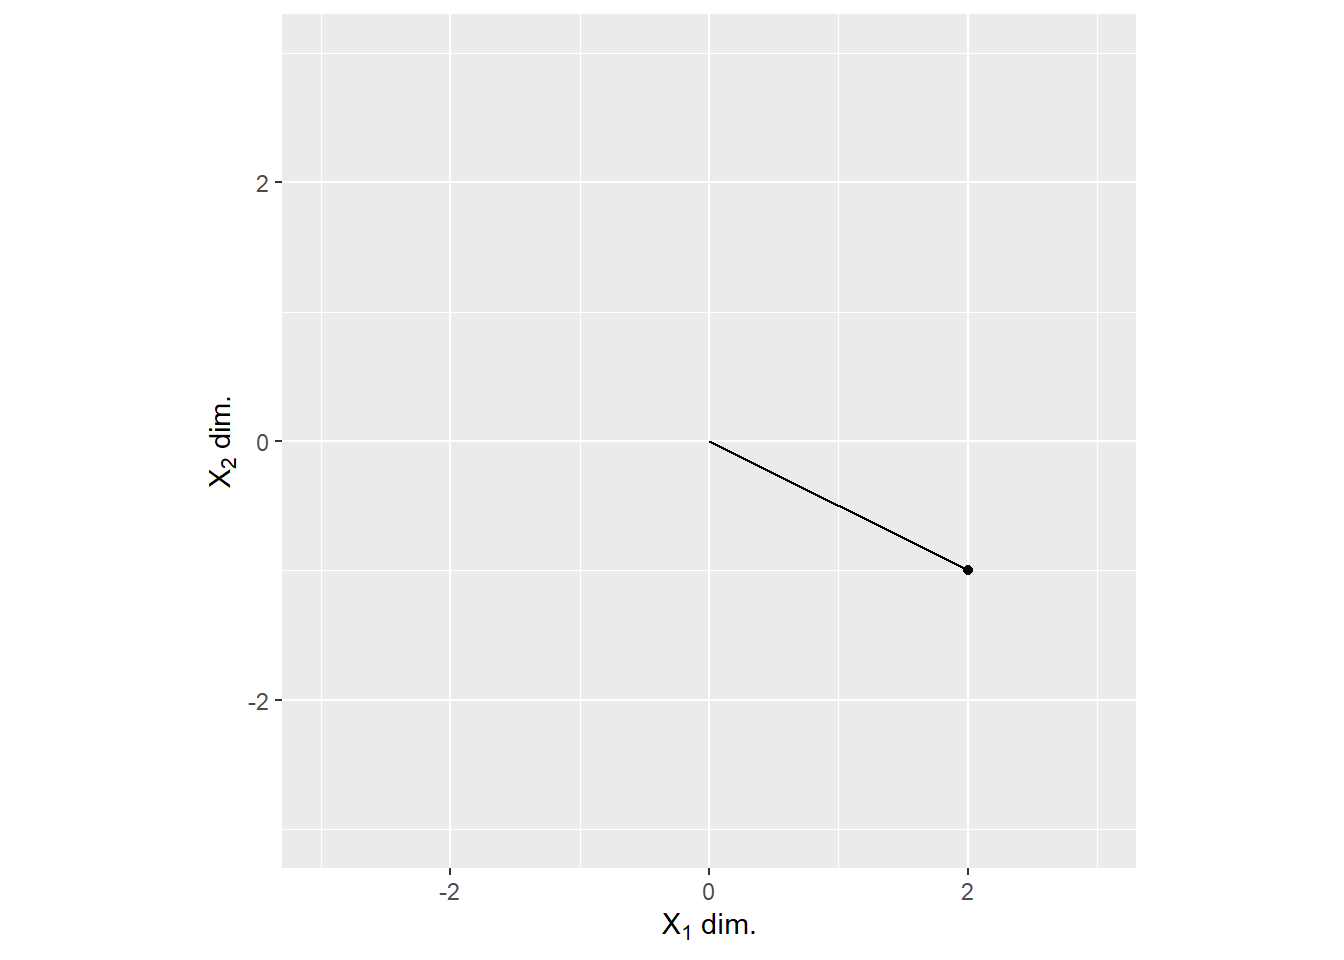
\includegraphics{cohen-linear-algebra_files/figure-latex/cb02-3/4-1.pdf}

\hypertarget{code-block-2.52.6}{%
\subsection*{Code block 2.5/2.6}\label{code-block-2.52.6}}
\addcontentsline{toc}{subsection}{Code block 2.5/2.6}

In R \emph{atomic} vectors are created via \texttt{c()} function but, technically, they are neither column, nor row vectors. \href{https://stat.ethz.ch/R-manual/R-devel/library/base/html/matmult.html}{Matrix multiplication manual} states that it ``\emph{multiplies two matrices, if they are conformable. If one argument is a vector, it will be promoted to either a row or column matrix to make the two arguments conformable. If both are vectors of the same length, it will return the inner product (as a matrix).}'' At the same time, \emph{transposing} an atomic vector \texttt{t(c(...))} transforms it into a single row matrix, thus a row vector, hinting that deep down an outcome of \texttt{c()} is a column vector.

To avoid ambiguity, I will use single row and single column matrices for, respectively, row and column vectors.

\begin{Shaded}
\begin{Highlighting}[]
\NormalTok{v1 \textless{}{-}}\StringTok{ }\KeywordTok{matrix}\NormalTok{(}\KeywordTok{c}\NormalTok{(}\DecValTok{2}\NormalTok{, }\DecValTok{5}\NormalTok{, }\DecValTok{5}\NormalTok{, }\DecValTok{7}\NormalTok{), }\DataTypeTok{nrow =} \DecValTok{1}\NormalTok{) }\CommentTok{\# row vector}
\NormalTok{v2 \textless{}{-}}\StringTok{ }\KeywordTok{matrix}\NormalTok{(}\KeywordTok{c}\NormalTok{(}\DecValTok{2}\NormalTok{, }\DecValTok{5}\NormalTok{, }\DecValTok{5}\NormalTok{, }\DecValTok{7}\NormalTok{), }\DataTypeTok{ncol =} \DecValTok{1}\NormalTok{) }\CommentTok{\# column vector}
\NormalTok{v3 \textless{}{-}}\StringTok{ }\KeywordTok{matrix}\NormalTok{(}\KeywordTok{c}\NormalTok{(}\DecValTok{2}\NormalTok{, }\DecValTok{5}\NormalTok{, }\DecValTok{5}\NormalTok{, }\DecValTok{7}\NormalTok{))           }\CommentTok{\# also a column vector}
\end{Highlighting}
\end{Shaded}

\hypertarget{code-block-2.72.8}{%
\subsection*{Code block 2.7/2.8}\label{code-block-2.72.8}}
\addcontentsline{toc}{subsection}{Code block 2.7/2.8}

\begin{Shaded}
\begin{Highlighting}[]
\NormalTok{v1 \textless{}{-}}\StringTok{ }\KeywordTok{matrix}\NormalTok{(}\KeywordTok{c}\NormalTok{(}\DecValTok{2}\NormalTok{, }\DecValTok{5}\NormalTok{, }\DecValTok{5}\NormalTok{, }\DecValTok{7}\NormalTok{), }\DataTypeTok{nrow =} \DecValTok{1}\NormalTok{) }\CommentTok{\# row vector}
\NormalTok{v1a \textless{}{-}}\StringTok{ }\KeywordTok{t}\NormalTok{(}\KeywordTok{c}\NormalTok{(}\DecValTok{2}\NormalTok{, }\DecValTok{5}\NormalTok{, }\DecValTok{5}\NormalTok{, }\DecValTok{7}\NormalTok{))               }\CommentTok{\# also a row vector}
\NormalTok{v2 \textless{}{-}}\StringTok{ }\KeywordTok{t}\NormalTok{(v1)                           }\CommentTok{\# column vector}
\end{Highlighting}
\end{Shaded}

\hypertarget{code-block-2.92.10}{%
\subsection*{Code block 2.9/2.10}\label{code-block-2.92.10}}
\addcontentsline{toc}{subsection}{Code block 2.9/2.10}

For this example, you can also use atomic vectors directly without turning them into a column vector / single column matrix.

\begin{Shaded}
\begin{Highlighting}[]
\NormalTok{v1 \textless{}{-}}\StringTok{ }\KeywordTok{matrix}\NormalTok{(}\KeywordTok{c}\NormalTok{(}\DecValTok{2}\NormalTok{, }\DecValTok{5}\NormalTok{, }\DecValTok{4}\NormalTok{, }\DecValTok{7}\NormalTok{), }\DataTypeTok{ncol=}\DecValTok{1}\NormalTok{)}
\NormalTok{v2 \textless{}{-}}\StringTok{ }\KeywordTok{matrix}\NormalTok{(}\KeywordTok{c}\NormalTok{(}\DecValTok{4}\NormalTok{, }\DecValTok{1}\NormalTok{, }\DecValTok{0}\NormalTok{, }\DecValTok{2}\NormalTok{), }\DataTypeTok{ncol=}\DecValTok{1}\NormalTok{)}
\NormalTok{v3 \textless{}{-}}\StringTok{ }\DecValTok{4} \OperatorTok{*}\StringTok{ }\NormalTok{v1  }\OperatorTok{{-}}\StringTok{ }\DecValTok{2} \OperatorTok{*}\StringTok{ }\NormalTok{v2}
\end{Highlighting}
\end{Shaded}

\hypertarget{chapter-3}{%
\section*{Chapter 3}\label{chapter-3}}
\addcontentsline{toc}{section}{Chapter 3}

\hypertarget{code-block-3.13.2}{%
\subsection*{Code block 3.1/3.2}\label{code-block-3.13.2}}
\addcontentsline{toc}{subsection}{Code block 3.1/3.2}

There is no \emph{explicit} dot product function in base R but there are multiple implementations in various libraries such as \href{https://github.com/cran/pracma}{pracma} used here.

\begin{Shaded}
\begin{Highlighting}[]
\NormalTok{v1 \textless{}{-}}\StringTok{ }\KeywordTok{matrix}\NormalTok{(}\KeywordTok{c}\NormalTok{(}\DecValTok{2}\NormalTok{, }\DecValTok{5}\NormalTok{, }\DecValTok{4}\NormalTok{, }\DecValTok{7}\NormalTok{), }\DataTypeTok{ncol=}\DecValTok{1}\NormalTok{)}
\NormalTok{v2 \textless{}{-}}\StringTok{ }\KeywordTok{matrix}\NormalTok{(}\KeywordTok{c}\NormalTok{(}\DecValTok{4}\NormalTok{, }\DecValTok{1}\NormalTok{, }\DecValTok{0}\NormalTok{, }\DecValTok{2}\NormalTok{), }\DataTypeTok{ncol=}\DecValTok{1}\NormalTok{)}
\NormalTok{dp \textless{}{-}}\StringTok{ }\NormalTok{pracma}\OperatorTok{::}\KeywordTok{dot}\NormalTok{(v1, v2)}
\end{Highlighting}
\end{Shaded}

However, a matrix multiplication of \emph{atomic} vectors (we can convert a matrix back to an atomic vector via \texttt{c()} or \texttt{as.vector()}) gives us the dot product (well, the \emph{inner} product, which is why the result is a 1-by-1 matrix).

\begin{Shaded}
\begin{Highlighting}[]
\NormalTok{dp \textless{}{-}}\StringTok{ }\KeywordTok{c}\NormalTok{(v1) }\OperatorTok{\%*\%}\StringTok{ }\KeywordTok{as.vector}\NormalTok{(v2)}
\end{Highlighting}
\end{Shaded}

\hypertarget{code-block-3.33.4}{%
\subsection*{Code block 3.3/3.4}\label{code-block-3.33.4}}
\addcontentsline{toc}{subsection}{Code block 3.3/3.4}

\begin{Shaded}
\begin{Highlighting}[]
\NormalTok{l1 \textless{}{-}}\StringTok{ }\DecValTok{1}
\NormalTok{l2 \textless{}{-}}\StringTok{ }\DecValTok{2}
\NormalTok{l3 \textless{}{-}}\StringTok{ }\DecValTok{{-}3}
\NormalTok{v1 \textless{}{-}}\StringTok{ }\KeywordTok{matrix}\NormalTok{(}\KeywordTok{c}\NormalTok{(}\DecValTok{4}\NormalTok{, }\DecValTok{5}\NormalTok{, }\DecValTok{1}\NormalTok{), }\DataTypeTok{ncol=}\DecValTok{1}\NormalTok{)}
\NormalTok{v2 \textless{}{-}}\StringTok{ }\KeywordTok{matrix}\NormalTok{(}\KeywordTok{c}\NormalTok{(}\OperatorTok{{-}}\DecValTok{4}\NormalTok{, }\DecValTok{0}\NormalTok{, }\DecValTok{{-}4}\NormalTok{), }\DataTypeTok{ncol=}\DecValTok{1}\NormalTok{)}
\NormalTok{v3 \textless{}{-}}\StringTok{ }\KeywordTok{matrix}\NormalTok{(}\KeywordTok{c}\NormalTok{(}\DecValTok{1}\NormalTok{, }\DecValTok{3}\NormalTok{, }\DecValTok{2}\NormalTok{), }\DataTypeTok{ncol=}\DecValTok{1}\NormalTok{)}
\NormalTok{l1 }\OperatorTok{*}\StringTok{ }\NormalTok{v1 }\OperatorTok{+}\StringTok{ }\NormalTok{l2 }\OperatorTok{*}\StringTok{ }\NormalTok{v2 }\OperatorTok{+}\StringTok{ }\NormalTok{l3 }\OperatorTok{*}\StringTok{ }\NormalTok{v3}
\end{Highlighting}
\end{Shaded}

\begin{verbatim}
##      [,1]
## [1,]   -7
## [2,]   -4
## [3,]  -13
\end{verbatim}

\hypertarget{code-block-3.53.6}{%
\subsection*{Code block 3.5/3.6}\label{code-block-3.53.6}}
\addcontentsline{toc}{subsection}{Code block 3.5/3.6}

To compute the outer product, we must use atomic vectors, thus I've skipped the whole creating-column-vector-as-a-matrix thing.

\begin{Shaded}
\begin{Highlighting}[]
\NormalTok{v1 \textless{}{-}}\StringTok{ }\KeywordTok{c}\NormalTok{(}\DecValTok{2}\NormalTok{, }\DecValTok{5}\NormalTok{, }\DecValTok{4}\NormalTok{, }\DecValTok{7}\NormalTok{)}
\NormalTok{v2 \textless{}{-}}\StringTok{ }\KeywordTok{c}\NormalTok{(}\DecValTok{4}\NormalTok{, }\DecValTok{1}\NormalTok{, }\DecValTok{0}\NormalTok{, }\DecValTok{2}\NormalTok{)}
\NormalTok{op \textless{}{-}}\StringTok{ }\KeywordTok{outer}\NormalTok{(v1, v2)}
\NormalTok{op \textless{}{-}}\StringTok{ }\NormalTok{v1 }\OperatorTok{\%o\%}\StringTok{ }\NormalTok{v2 }\CommentTok{\# alternative call as operation}
\end{Highlighting}
\end{Shaded}

Alternatively, if we do start with vectors as single column matrices\ldots{}

\begin{Shaded}
\begin{Highlighting}[]
\NormalTok{v1 \textless{}{-}}\StringTok{ }\KeywordTok{matrix}\NormalTok{(}\KeywordTok{c}\NormalTok{(}\DecValTok{2}\NormalTok{, }\DecValTok{5}\NormalTok{, }\DecValTok{4}\NormalTok{, }\DecValTok{7}\NormalTok{), }\DataTypeTok{ncol=}\DecValTok{1}\NormalTok{)}
\NormalTok{v2 \textless{}{-}}\StringTok{ }\KeywordTok{matrix}\NormalTok{(}\KeywordTok{c}\NormalTok{(}\DecValTok{4}\NormalTok{, }\DecValTok{1}\NormalTok{, }\DecValTok{0}\NormalTok{, }\DecValTok{2}\NormalTok{), }\DataTypeTok{ncol=}\DecValTok{1}\NormalTok{)}
\NormalTok{op \textless{}{-}}\StringTok{ }\KeywordTok{outer}\NormalTok{(}\KeywordTok{c}\NormalTok{(v1), }\KeywordTok{c}\NormalTok{(v2))}
\NormalTok{op \textless{}{-}}\StringTok{ }\KeywordTok{c}\NormalTok{(v1) }\OperatorTok{\%o\%}\StringTok{ }\KeywordTok{c}\NormalTok{(v2) }\CommentTok{\# alternative call as operation}
\end{Highlighting}
\end{Shaded}

\hypertarget{code-block-3.73.8}{%
\subsection*{Code block 3.7/3.8}\label{code-block-3.73.8}}
\addcontentsline{toc}{subsection}{Code block 3.7/3.8}

\begin{Shaded}
\begin{Highlighting}[]
\NormalTok{v1 \textless{}{-}}\StringTok{ }\KeywordTok{matrix}\NormalTok{(}\KeywordTok{c}\NormalTok{(}\DecValTok{2}\NormalTok{, }\DecValTok{5}\NormalTok{, }\DecValTok{4}\NormalTok{, }\DecValTok{7}\NormalTok{), }\DataTypeTok{ncol=}\DecValTok{1}\NormalTok{)}
\NormalTok{v2 \textless{}{-}}\StringTok{ }\KeywordTok{matrix}\NormalTok{(}\KeywordTok{c}\NormalTok{(}\DecValTok{4}\NormalTok{, }\DecValTok{1}\NormalTok{, }\DecValTok{0}\NormalTok{, }\DecValTok{2}\NormalTok{), }\DataTypeTok{ncol=}\DecValTok{1}\NormalTok{)}
\NormalTok{v3 \textless{}{-}}\StringTok{ }\NormalTok{v1 }\OperatorTok{*}\StringTok{ }\NormalTok{v2}
\end{Highlighting}
\end{Shaded}

\hypertarget{code-block-3.93.10}{%
\subsection*{Code block 3.9/3.10}\label{code-block-3.93.10}}
\addcontentsline{toc}{subsection}{Code block 3.9/3.10}

Please note that you need to explicitly specify the 2-norm via \texttt{type="2"}, as the \emph{one norm} is used by default.

\begin{Shaded}
\begin{Highlighting}[]
\NormalTok{v \textless{}{-}}\StringTok{ }\KeywordTok{matrix}\NormalTok{(}\KeywordTok{c}\NormalTok{(}\DecValTok{2}\NormalTok{, }\DecValTok{5}\NormalTok{, }\DecValTok{4}\NormalTok{, }\DecValTok{7}\NormalTok{), }\DataTypeTok{ncol=}\DecValTok{1}\NormalTok{)}
\NormalTok{vMag \textless{}{-}}\StringTok{ }\KeywordTok{norm}\NormalTok{(v, }\DataTypeTok{type=}\StringTok{"2"}\NormalTok{)}
\NormalTok{v\_unit \textless{}{-}}\StringTok{ }\NormalTok{v }\OperatorTok{/}\StringTok{ }\NormalTok{vMag}
\end{Highlighting}
\end{Shaded}

\hypertarget{chapter-5}{%
\section*{Chapter 5}\label{chapter-5}}
\addcontentsline{toc}{section}{Chapter 5}

\hypertarget{code-block-5.15.2}{%
\subsection*{Code block 5.1/5.2}\label{code-block-5.15.2}}
\addcontentsline{toc}{subsection}{Code block 5.1/5.2}

There is only one way to transpose a matrix in R: via function \href{https://stat.ethz.ch/R-manual/R-devel/library/base/html/t.html}{t()}.

\begin{Shaded}
\begin{Highlighting}[]
\NormalTok{A \textless{}{-}}\StringTok{ }\KeywordTok{matrix}\NormalTok{(}\KeywordTok{runif}\NormalTok{(}\DataTypeTok{n=}\DecValTok{2}\OperatorTok{*}\DecValTok{5}\NormalTok{), }\DataTypeTok{nrow=}\DecValTok{2}\NormalTok{, }\DataTypeTok{ncol=}\DecValTok{5}\NormalTok{)}
\NormalTok{At1 \textless{}{-}}\StringTok{ }\KeywordTok{t}\NormalTok{(A)}
\end{Highlighting}
\end{Shaded}

\hypertarget{code-block-5.35.4}{%
\subsection*{Code block 5.3/5.4}\label{code-block-5.35.4}}
\addcontentsline{toc}{subsection}{Code block 5.3/5.4}

\begin{Shaded}
\begin{Highlighting}[]
\NormalTok{I \textless{}{-}}\StringTok{ }\KeywordTok{diag}\NormalTok{(}\DecValTok{4}\NormalTok{)}
\NormalTok{O \textless{}{-}}\StringTok{ }\KeywordTok{matrix}\NormalTok{(}\DecValTok{1}\NormalTok{, }\DataTypeTok{nrow=}\DecValTok{4}\NormalTok{, }\DataTypeTok{ncol=}\DecValTok{1}\NormalTok{) }\CommentTok{\# or rep(1, times=4) to create an atomic vector}
\NormalTok{Z \textless{}{-}}\StringTok{ }\KeywordTok{matrix}\NormalTok{(}\DecValTok{0}\NormalTok{, }\DataTypeTok{nrow=}\DecValTok{4}\NormalTok{, }\DataTypeTok{ncol=}\DecValTok{4}\NormalTok{)}
\end{Highlighting}
\end{Shaded}

\hypertarget{code-block-5.55.6}{%
\subsection*{Code block 5.5/5.6}\label{code-block-5.55.6}}
\addcontentsline{toc}{subsection}{Code block 5.5/5.6}

\begin{Shaded}
\begin{Highlighting}[]
\NormalTok{D \textless{}{-}}\StringTok{ }\KeywordTok{diag}\NormalTok{(}\KeywordTok{c}\NormalTok{(}\DecValTok{1}\NormalTok{, }\DecValTok{2}\NormalTok{, }\DecValTok{3}\NormalTok{, }\DecValTok{5}\NormalTok{))  }\CommentTok{\# diagonal matrix}
\NormalTok{R \textless{}{-}}\StringTok{ }\KeywordTok{matrix}\NormalTok{(}\KeywordTok{runif}\NormalTok{(}\DataTypeTok{n =} \DecValTok{3} \OperatorTok{*}\StringTok{ }\DecValTok{4}\NormalTok{), }\DataTypeTok{nrow=}\DecValTok{3}\NormalTok{, }\DataTypeTok{ncol=}\DecValTok{4}\NormalTok{)}
\NormalTok{d \textless{}{-}}\StringTok{ }\KeywordTok{diag}\NormalTok{(R) }\CommentTok{\# diagonal elements}
\end{Highlighting}
\end{Shaded}

\hypertarget{code-block-5.75.8}{%
\subsection*{Code block 5.7/5.8}\label{code-block-5.75.8}}
\addcontentsline{toc}{subsection}{Code block 5.7/5.8}

In r \href{https://stat.ethz.ch/R-manual/R-devel/library/base/html/cbind.html}{cbind()} and \href{https://stat.ethz.ch/R-manual/R-devel/library/base/html/cbind.html}{rbind()} concatenate, respectively, by column and row.

\begin{Shaded}
\begin{Highlighting}[]
\NormalTok{A \textless{}{-}}\StringTok{ }\KeywordTok{matrix}\NormalTok{(}\KeywordTok{runif}\NormalTok{(}\DataTypeTok{n =} \DecValTok{3} \OperatorTok{*}\StringTok{ }\DecValTok{5}\NormalTok{), }\DataTypeTok{nrow=}\DecValTok{3}\NormalTok{, }\DataTypeTok{ncol=}\DecValTok{5}\NormalTok{)}
\NormalTok{B \textless{}{-}}\StringTok{ }\KeywordTok{matrix}\NormalTok{(}\KeywordTok{runif}\NormalTok{(}\DataTypeTok{n =} \DecValTok{3} \OperatorTok{*}\StringTok{ }\DecValTok{4}\NormalTok{), }\DataTypeTok{nrow=}\DecValTok{3}\NormalTok{, }\DataTypeTok{ncol=}\DecValTok{4}\NormalTok{)}
\NormalTok{AB \textless{}{-}}\StringTok{ }\KeywordTok{cbind}\NormalTok{(A, B)}
\end{Highlighting}
\end{Shaded}

\hypertarget{code-block-5.95.10}{%
\subsection*{Code block 5.9/5.10}\label{code-block-5.95.10}}
\addcontentsline{toc}{subsection}{Code block 5.9/5.10}

There are two ways to compute lower and upper triangular parts of a matrix. First, to use \texttt{tril()} and \texttt{triu()} function from \emph{pracma} library.

\begin{Shaded}
\begin{Highlighting}[]
\NormalTok{A \textless{}{-}}\StringTok{ }\KeywordTok{matrix}\NormalTok{(}\KeywordTok{runif}\NormalTok{(}\DataTypeTok{n =} \DecValTok{5} \OperatorTok{*}\StringTok{ }\DecValTok{5}\NormalTok{), }\DataTypeTok{nrow=}\DecValTok{5}\NormalTok{, }\DataTypeTok{ncol=}\DecValTok{5}\NormalTok{)}
\NormalTok{L \textless{}{-}}\StringTok{ }\NormalTok{pracma}\OperatorTok{::}\KeywordTok{tril}\NormalTok{(A)}
\NormalTok{U \textless{}{-}}\StringTok{ }\NormalTok{pracma}\OperatorTok{::}\KeywordTok{triu}\NormalTok{(A)}
\end{Highlighting}
\end{Shaded}

Alternatively, you can use base R functions \href{https://stat.ethz.ch/R-manual/R-devel/library/base/html/lower.tri.html}{lower.tri()} and \texttt{upper.tri()} that give you a matrix of the same size with \emph{logical} values indicating whether an element belongs to, respectively, lower or upper triangle. Note that by default, the diagonal \emph{is not} included!

\begin{Shaded}
\begin{Highlighting}[]
\NormalTok{A \textless{}{-}}\StringTok{ }\KeywordTok{matrix}\NormalTok{(}\KeywordTok{runif}\NormalTok{(}\DataTypeTok{n =} \DecValTok{5} \OperatorTok{*}\StringTok{ }\DecValTok{5}\NormalTok{), }\DataTypeTok{nrow=}\DecValTok{5}\NormalTok{, }\DataTypeTok{ncol=}\DecValTok{5}\NormalTok{)}

\NormalTok{L \textless{}{-}}\StringTok{ }\NormalTok{A}
\CommentTok{\# by setting the UPPER triangular part to 0, we get the LOWER triangular part and the diagonal}
\NormalTok{L[}\KeywordTok{upper.tri}\NormalTok{(L)] \textless{}{-}}\StringTok{ }\DecValTok{0}

\NormalTok{U \textless{}{-}}\StringTok{ }\NormalTok{A}
\CommentTok{\# by setting the LOWER triangular part to 0, we get the UPPER triangular part and the diagonal}
\NormalTok{U[}\KeywordTok{lower.tri}\NormalTok{(U)] \textless{}{-}}\StringTok{ }\DecValTok{0}
\end{Highlighting}
\end{Shaded}

\hypertarget{code-block-5.115.12}{%
\subsection*{Code block 5.11/5.12}\label{code-block-5.115.12}}
\addcontentsline{toc}{subsection}{Code block 5.11/5.12}

Note that there is a \texttt{toeplitz()} function in \emph{stats} (base R) and \texttt{Topelitz()} (note the first capital letter) in \emph{pracma} library. Here, I use base R version.

\begin{Shaded}
\begin{Highlighting}[]
\NormalTok{t \textless{}{-}}\StringTok{ }\KeywordTok{c}\NormalTok{(}\DecValTok{1}\NormalTok{, }\DecValTok{2}\NormalTok{, }\DecValTok{3}\NormalTok{, }\DecValTok{4}\NormalTok{)}
\NormalTok{T \textless{}{-}}\StringTok{ }\NormalTok{stats}\OperatorTok{::}\KeywordTok{toeplitz}\NormalTok{(t)}
\NormalTok{H \textless{}{-}}\StringTok{ }\NormalTok{pracma}\OperatorTok{::}\KeywordTok{hankel}\NormalTok{(t, }\DataTypeTok{b=} \KeywordTok{c}\NormalTok{(t[}\OperatorTok{{-}}\DecValTok{1}\NormalTok{], t[}\DecValTok{1}\NormalTok{]))}
\end{Highlighting}
\end{Shaded}

\begin{verbatim}
## Warning in pracma::hankel(t, b = c(t[-1], t[1])): a[n] not equal to b[1], b[1]
## set to a[n].
\end{verbatim}

\hypertarget{code-block-5.135.14}{%
\subsection*{Code block 5.13/5.14}\label{code-block-5.135.14}}
\addcontentsline{toc}{subsection}{Code block 5.13/5.14}

\begin{Shaded}
\begin{Highlighting}[]
\NormalTok{l \textless{}{-}}\StringTok{ }\FloatTok{0.01}
\NormalTok{I \textless{}{-}}\StringTok{ }\KeywordTok{diag}\NormalTok{(}\DecValTok{4}\NormalTok{)}
\NormalTok{A \textless{}{-}}\StringTok{ }\KeywordTok{matrix}\NormalTok{(}\KeywordTok{runif}\NormalTok{(}\DecValTok{4} \OperatorTok{*}\StringTok{ }\DecValTok{4}\NormalTok{), }\DataTypeTok{nrow=}\DecValTok{4}\NormalTok{, }\DataTypeTok{ncol=}\DecValTok{4}\NormalTok{)}
\NormalTok{As \textless{}{-}}\StringTok{ }\NormalTok{A }\OperatorTok{+}\StringTok{ }\NormalTok{l }\OperatorTok{*}\StringTok{ }\NormalTok{I}
\end{Highlighting}
\end{Shaded}

\hypertarget{code-block-5.155.16}{%
\subsection*{Code block 5.15/5.16}\label{code-block-5.155.16}}
\addcontentsline{toc}{subsection}{Code block 5.15/5.16}

Base R does not implement trace function, as it is simply a \texttt{sum(diag(M))}. However, you can use \texttt{Trace()} from \emph{pracma} library.

\begin{Shaded}
\begin{Highlighting}[]
\NormalTok{A \textless{}{-}}\StringTok{ }\KeywordTok{matrix}\NormalTok{(}\KeywordTok{runif}\NormalTok{(}\DecValTok{4} \OperatorTok{*}\StringTok{ }\DecValTok{4}\NormalTok{), }\DataTypeTok{nrow=}\DecValTok{4}\NormalTok{, }\DataTypeTok{ncol=}\DecValTok{4}\NormalTok{)}
\NormalTok{tr \textless{}{-}}\StringTok{ }\NormalTok{pracma}\OperatorTok{::}\KeywordTok{Trace}\NormalTok{(A)}
\end{Highlighting}
\end{Shaded}

\hypertarget{chapter-6}{%
\section*{Chapter 6}\label{chapter-6}}
\addcontentsline{toc}{section}{Chapter 6}

\hypertarget{code-block-6.16.2}{%
\subsection*{Code block 6.1/6.2}\label{code-block-6.16.2}}
\addcontentsline{toc}{subsection}{Code block 6.1/6.2}

\begin{Shaded}
\begin{Highlighting}[]
\NormalTok{M1 \textless{}{-}}\StringTok{ }\KeywordTok{matrix}\NormalTok{(}\KeywordTok{runif}\NormalTok{(}\DataTypeTok{n=}\DecValTok{4}\OperatorTok{*}\DecValTok{3}\NormalTok{), }\DataTypeTok{nrow=}\DecValTok{4}\NormalTok{, }\DataTypeTok{ncol=}\DecValTok{3}\NormalTok{)}
\NormalTok{M2 \textless{}{-}}\StringTok{ }\KeywordTok{matrix}\NormalTok{(}\KeywordTok{runif}\NormalTok{(}\DataTypeTok{n=}\DecValTok{3}\OperatorTok{*}\DecValTok{5}\NormalTok{), }\DataTypeTok{nrow=}\DecValTok{3}\NormalTok{, }\DataTypeTok{ncol=}\DecValTok{5}\NormalTok{)}
\NormalTok{C \textless{}{-}}\StringTok{ }\NormalTok{M1 }\OperatorTok{\%*\%}\StringTok{ }\NormalTok{M2}
\end{Highlighting}
\end{Shaded}

\hypertarget{code-block-6.36.4}{%
\subsection*{Code block 6.3/6.4}\label{code-block-6.36.4}}
\addcontentsline{toc}{subsection}{Code block 6.3/6.4}

\begin{Shaded}
\begin{Highlighting}[]
\NormalTok{A \textless{}{-}}\StringTok{ }\KeywordTok{matrix}\NormalTok{(}\KeywordTok{runif}\NormalTok{(}\DataTypeTok{n=}\DecValTok{2}\OperatorTok{*}\DecValTok{2}\NormalTok{), }\DataTypeTok{nrow=}\DecValTok{2}\NormalTok{, }\DataTypeTok{ncol=}\DecValTok{2}\NormalTok{)}
\NormalTok{B \textless{}{-}}\StringTok{ }\KeywordTok{matrix}\NormalTok{(}\KeywordTok{runif}\NormalTok{(}\DataTypeTok{n=}\DecValTok{2}\OperatorTok{*}\DecValTok{2}\NormalTok{), }\DataTypeTok{nrow=}\DecValTok{2}\NormalTok{, }\DataTypeTok{ncol=}\DecValTok{2}\NormalTok{)}
\NormalTok{C1 \textless{}{-}}\StringTok{ }\NormalTok{A }\OperatorTok{\%*\%}\StringTok{ }\NormalTok{B}
\NormalTok{C2 \textless{}{-}}\StringTok{ }\NormalTok{B }\OperatorTok{\%*\%}\StringTok{ }\NormalTok{A}
\end{Highlighting}
\end{Shaded}

\hypertarget{code-block-6.56.6}{%
\subsection*{Code block 6.5/6.6}\label{code-block-6.56.6}}
\addcontentsline{toc}{subsection}{Code block 6.5/6.6}

\begin{Shaded}
\begin{Highlighting}[]
\NormalTok{M1 \textless{}{-}}\StringTok{ }\KeywordTok{matrix}\NormalTok{(}\KeywordTok{runif}\NormalTok{(}\DataTypeTok{n=}\DecValTok{4}\OperatorTok{*}\DecValTok{3}\NormalTok{), }\DataTypeTok{nrow=}\DecValTok{4}\NormalTok{, }\DataTypeTok{ncol=}\DecValTok{3}\NormalTok{)}
\NormalTok{M2 \textless{}{-}}\StringTok{ }\KeywordTok{matrix}\NormalTok{(}\KeywordTok{runif}\NormalTok{(}\DataTypeTok{n=}\DecValTok{4}\OperatorTok{*}\DecValTok{3}\NormalTok{), }\DataTypeTok{nrow=}\DecValTok{4}\NormalTok{, }\DataTypeTok{ncol=}\DecValTok{3}\NormalTok{)}
\NormalTok{C \textless{}{-}}\StringTok{ }\NormalTok{M1 }\OperatorTok{*}\StringTok{ }\NormalTok{M2}
\end{Highlighting}
\end{Shaded}

\hypertarget{code-block-6.76.8}{%
\subsection*{Code block 6.7/6.8}\label{code-block-6.76.8}}
\addcontentsline{toc}{subsection}{Code block 6.7/6.8}

Note that by default, matrix is constructed by column. To match the code, we need to use \texttt{byrow=TRUE} option.

\begin{Shaded}
\begin{Highlighting}[]
\NormalTok{A \textless{}{-}}\StringTok{ }\KeywordTok{matrix}\NormalTok{(}\KeywordTok{c}\NormalTok{(}\DecValTok{1}\NormalTok{, }\DecValTok{2}\NormalTok{, }\DecValTok{3}\NormalTok{, }\DecValTok{4}\NormalTok{, }\DecValTok{5}\NormalTok{, }\DecValTok{6}\NormalTok{), }\DataTypeTok{nrow=}\DecValTok{2}\NormalTok{, }\DataTypeTok{byrow =} \OtherTok{TRUE}\NormalTok{)}
\KeywordTok{c}\NormalTok{(A)}
\end{Highlighting}
\end{Shaded}

\begin{verbatim}
## [1] 1 4 2 5 3 6
\end{verbatim}

\hypertarget{code-block-6.96.10}{%
\subsection*{Code block 6.9/6.10}\label{code-block-6.96.10}}
\addcontentsline{toc}{subsection}{Code block 6.9/6.10}

\begin{Shaded}
\begin{Highlighting}[]
\NormalTok{A \textless{}{-}}\StringTok{ }\KeywordTok{matrix}\NormalTok{(}\KeywordTok{runif}\NormalTok{(}\DataTypeTok{n=}\DecValTok{4}\OperatorTok{*}\DecValTok{3}\NormalTok{), }\DataTypeTok{nrow=}\DecValTok{4}\NormalTok{, }\DataTypeTok{ncol=}\DecValTok{3}\NormalTok{)}
\NormalTok{B \textless{}{-}}\StringTok{ }\KeywordTok{matrix}\NormalTok{(}\KeywordTok{runif}\NormalTok{(}\DataTypeTok{n=}\DecValTok{4}\OperatorTok{*}\DecValTok{3}\NormalTok{), }\DataTypeTok{nrow=}\DecValTok{4}\NormalTok{, }\DataTypeTok{ncol=}\DecValTok{3}\NormalTok{)}
\NormalTok{f \textless{}{-}}\StringTok{ }\NormalTok{pracma}\OperatorTok{::}\KeywordTok{Trace}\NormalTok{(}\KeywordTok{t}\NormalTok{(A) }\OperatorTok{\%*\%}\StringTok{ }\NormalTok{B)}
\end{Highlighting}
\end{Shaded}

\hypertarget{code-block-6.116.12}{%
\subsection*{Code block 6.11/6.12}\label{code-block-6.116.12}}
\addcontentsline{toc}{subsection}{Code block 6.11/6.12}

\begin{Shaded}
\begin{Highlighting}[]
\NormalTok{A \textless{}{-}}\StringTok{ }\KeywordTok{matrix}\NormalTok{(}\KeywordTok{runif}\NormalTok{(}\DataTypeTok{n=}\DecValTok{4}\OperatorTok{*}\DecValTok{3}\NormalTok{), }\DataTypeTok{nrow=}\DecValTok{4}\NormalTok{, }\DataTypeTok{ncol=}\DecValTok{3}\NormalTok{)}
\KeywordTok{norm}\NormalTok{(A, }\DataTypeTok{type=}\StringTok{"F"}\NormalTok{)}
\end{Highlighting}
\end{Shaded}

\begin{verbatim}
## [1] 1.681079
\end{verbatim}

\hypertarget{chapter-7}{%
\section*{Chapter 7}\label{chapter-7}}
\addcontentsline{toc}{section}{Chapter 7}

\hypertarget{code-block-7.17.2}{%
\subsection*{Code block 7.1/7.2}\label{code-block-7.17.2}}
\addcontentsline{toc}{subsection}{Code block 7.1/7.2}

You can use \texttt{Rank()} from the \emph{pracma} library. Alternatively, you can use \texttt{rankMatrix()} function from the \emph{Matrix} library, which in addition to the rank itself, returns information on the method used to estimate the rank via attributes.

\begin{Shaded}
\begin{Highlighting}[]
\NormalTok{A \textless{}{-}}\StringTok{ }\KeywordTok{matrix}\NormalTok{(}\KeywordTok{runif}\NormalTok{(}\DataTypeTok{n=}\DecValTok{3}\OperatorTok{*}\DecValTok{6}\NormalTok{), }\DataTypeTok{nrow=}\DecValTok{3}\NormalTok{, }\DataTypeTok{ncol=}\DecValTok{6}\NormalTok{)}
\NormalTok{r1 \textless{}{-}}\StringTok{ }\NormalTok{pracma}\OperatorTok{::}\KeywordTok{Rank}\NormalTok{(A)}
\NormalTok{r2 \textless{}{-}}\StringTok{ }\NormalTok{Matrix}\OperatorTok{::}\KeywordTok{rankMatrix}\NormalTok{(A)}
\end{Highlighting}
\end{Shaded}

\hypertarget{code-block-7.37.4}{%
\subsection*{Code block 7.3/7.4}\label{code-block-7.37.4}}
\addcontentsline{toc}{subsection}{Code block 7.3/7.4}

\begin{Shaded}
\begin{Highlighting}[]
\NormalTok{s \textless{}{-}}\StringTok{ }\KeywordTok{runif}\NormalTok{(}\DataTypeTok{n=}\DecValTok{1}\NormalTok{)}
\NormalTok{A \textless{}{-}}\StringTok{ }\KeywordTok{matrix}\NormalTok{(}\KeywordTok{runif}\NormalTok{(}\DataTypeTok{n=}\DecValTok{3}\OperatorTok{*}\DecValTok{5}\NormalTok{), }\DataTypeTok{nrow=}\DecValTok{3}\NormalTok{, }\DataTypeTok{ncol=}\DecValTok{5}\NormalTok{)}
\NormalTok{r1 \textless{}{-}}\StringTok{ }\NormalTok{pracma}\OperatorTok{::}\KeywordTok{Rank}\NormalTok{(A)}
\NormalTok{r2 \textless{}{-}}\StringTok{ }\NormalTok{pracma}\OperatorTok{::}\KeywordTok{Rank}\NormalTok{(s }\OperatorTok{*}\StringTok{ }\NormalTok{A)}
\KeywordTok{print}\NormalTok{(}\KeywordTok{c}\NormalTok{(r1, r2))}
\end{Highlighting}
\end{Shaded}

\begin{verbatim}
## [1] 3 3
\end{verbatim}

\hypertarget{code-block-7.57.6}{%
\subsection*{Code block 7.5/7.6}\label{code-block-7.57.6}}
\addcontentsline{toc}{subsection}{Code block 7.5/7.6}

Source code for \texttt{Rank()} function from \emph{pracma} library.

\begin{Shaded}
\begin{Highlighting}[]
\NormalTok{pracma}\OperatorTok{::}\NormalTok{Rank}
\end{Highlighting}
\end{Shaded}

\begin{verbatim}
## function (M) 
## {
##     if (length(M) == 0) 
##         return(0)
##     if (!is.numeric(M)) 
##         stop("Argument 'M' must be a numeric matrix.")
##     if (is.vector(M)) 
##         M <- matrix(c(M), nrow = length(M), ncol = 1)
##     r1 <- qr(M)$rank
##     sigma <- svd(M)$d
##     tol <- max(dim(M)) * max(sigma) * .Machine$double.eps
##     r2 <- sum(sigma > tol)
##     if (r1 != r2) 
##         warning("Rank calculation may be problematic.")
##     return(r2)
## }
## <bytecode: 0x0000000018e9f6b0>
## <environment: namespace:pracma>
\end{verbatim}

Source code for \texttt{rankMatrix()} function from \emph{Matrix} library.

\begin{Shaded}
\begin{Highlighting}[]
\NormalTok{Matrix}\OperatorTok{::}\NormalTok{rankMatrix}
\end{Highlighting}
\end{Shaded}

\begin{verbatim}
## function (x, tol = NULL, method = c("tolNorm2", "qr.R", "qrLINPACK", 
##     "qr", "useGrad", "maybeGrad"), sval = svd(x, 0, 0)$d, warn.t = TRUE) 
## {
##     stopifnot(length(d <- dim(x)) == 2)
##     p <- min(d)
##     method <- match.arg(method)
##     if (useGrad <- (method %in% c("useGrad", "maybeGrad"))) {
##         stopifnot(length(sval) == p, diff(sval) <= 0)
##         if (sval[1] == 0) {
##             useGrad <- FALSE
##             method <- eval(formals()[["method"]])[[1]]
##         }
##         else {
##             ln.av <- log(abs(sval))
##             diff1 <- diff(ln.av)
##             if (method == "maybeGrad") {
##                 grad <- (min(ln.av) - max(ln.av))/p
##                 useGrad <- !is.na(grad) && min(diff1) <= min(-3, 
##                   10 * grad)
##             }
##         }
##     }
##     if (!useGrad) {
##         x.dense <- is.numeric(x) || is(x, "denseMatrix")
##         if ((Meth <- method) == "qr") 
##             method <- if (x.dense) 
##                 "qrLINPACK"
##             else "qr.R"
##         else Meth <- substr(method, 1, 2)
##         if (Meth == "qr") {
##             if (is.null(tol)) 
##                 tol <- max(d) * .Machine$double.eps
##         }
##         else {
##             if (is.null(tol)) {
##                 if (!x.dense && missing(sval) && prod(d) >= 100000L) 
##                   warning(gettextf("rankMatrix(<large sparse Matrix>, method = '%s') coerces to dense matrix.\n Probably should rather use method = 'qr' !?", 
##                     method), immediate. = TRUE, domain = NA)
##                 stopifnot(diff(sval) <= 0)
##                 tol <- max(d) * .Machine$double.eps
##             }
##             else stopifnot((tol <- as.numeric(tol)[[1]]) >= 0)
##         }
##     }
##     structure(if (useGrad) 
##         which.min(diff1)
##     else if (Meth == "qr") {
##         if ((do.t <- (d[1L] < d[2L])) && warn.t) 
##             warning(gettextf("rankMatrix(x, method='qr'): computing t(x) as nrow(x) < ncol(x)"))
##         q.r <- qr(if (do.t) 
##             t(x)
##         else x, tol = tol, LAPACK = method != "qrLINPACK")
##         if (x.dense && (method == "qrLINPACK")) 
##             q.r$rank
##         else {
##             diagR <- if (x.dense) 
##                 diag(q.r$qr)
##             else diag(q.r@R)
##             d.i <- abs(diagR)
##             if ((mdi <- max(d.i)) > 0) 
##                 sum(d.i >= tol * mdi)
##             else 0L
##         }
##     }
##     else if (sval[1] > 0) 
##         sum(sval >= tol * sval[1])
##     else 0L, method = method, useGrad = useGrad, tol = if (useGrad) 
##         NA
##     else tol)
## }
## <bytecode: 0x0000000020c79a78>
## <environment: namespace:Matrix>
\end{verbatim}

\hypertarget{chapter-8}{%
\section*{Chapter 8}\label{chapter-8}}
\addcontentsline{toc}{section}{Chapter 8}

\hypertarget{code-block-8.18.2}{%
\subsection*{Code block 8.1/8.2}\label{code-block-8.18.2}}
\addcontentsline{toc}{subsection}{Code block 8.1/8.2}

\begin{Shaded}
\begin{Highlighting}[]
\NormalTok{A \textless{}{-}}\StringTok{ }\KeywordTok{matrix}\NormalTok{(}\KeywordTok{runif}\NormalTok{(}\DataTypeTok{n=}\DecValTok{3}\OperatorTok{*}\DecValTok{4}\NormalTok{), }\DataTypeTok{nrow=}\DecValTok{3}\NormalTok{, }\DataTypeTok{ncol=}\DecValTok{4}\NormalTok{)}
\NormalTok{pracma}\OperatorTok{::}\KeywordTok{nullspace}\NormalTok{(A)}
\end{Highlighting}
\end{Shaded}

\begin{verbatim}
##            [,1]
## [1,] -0.4056543
## [2,]  0.2980013
## [3,] -0.7448863
## [4,]  0.4379317
\end{verbatim}

\hypertarget{chapter-9}{%
\section*{Chapter 9}\label{chapter-9}}
\addcontentsline{toc}{section}{Chapter 9}

\hypertarget{code-block-9.19.2}{%
\subsection*{Code block 9.1/9.2}\label{code-block-9.19.2}}
\addcontentsline{toc}{subsection}{Code block 9.1/9.2}

\begin{Shaded}
\begin{Highlighting}[]
\NormalTok{z \textless{}{-}}\StringTok{ }\KeywordTok{complex}\NormalTok{(}\DataTypeTok{real=}\DecValTok{3}\NormalTok{, }\DataTypeTok{imaginary=}\DecValTok{4}\NormalTok{)}
\NormalTok{Z \textless{}{-}}\StringTok{ }\KeywordTok{complex}\NormalTok{(}\DataTypeTok{length.out=}\DecValTok{2}\NormalTok{, }\DataTypeTok{real=}\DecValTok{0}\NormalTok{, }\DataTypeTok{imaginary=}\DecValTok{0}\NormalTok{)}
\NormalTok{Z[}\DecValTok{1}\NormalTok{] \textless{}{-}}\StringTok{ }\DecValTok{3} \OperatorTok{+}\StringTok{ }\NormalTok{4i}
\end{Highlighting}
\end{Shaded}

\hypertarget{code-block-9.39.4}{%
\subsection*{Code block 9.3/9.4}\label{code-block-9.39.4}}
\addcontentsline{toc}{subsection}{Code block 9.3/9.4}

Base R does not have a function that generates random integers on the interval. I will use \texttt{sample()} with replacement from the range of integers to replicate this. Also note that I have renamed \texttt{i} to \texttt{im} to minimize the confusion.

\begin{Shaded}
\begin{Highlighting}[]
\NormalTok{r \textless{}{-}}\StringTok{ }\KeywordTok{sample}\NormalTok{(}\OperatorTok{{-}}\DecValTok{3}\OperatorTok{:}\DecValTok{4}\NormalTok{, }\DataTypeTok{size=}\DecValTok{3}\NormalTok{, }\DataTypeTok{replace =} \OtherTok{TRUE}\NormalTok{)}
\NormalTok{im \textless{}{-}}\StringTok{ }\KeywordTok{sample}\NormalTok{(}\OperatorTok{{-}}\DecValTok{3}\OperatorTok{:}\DecValTok{4}\NormalTok{, }\DataTypeTok{size=}\DecValTok{3}\NormalTok{, }\DataTypeTok{replace =} \OtherTok{TRUE}\NormalTok{)}
\NormalTok{Z \textless{}{-}}\StringTok{ }\NormalTok{r }\OperatorTok{+}\StringTok{ }\NormalTok{im }\OperatorTok{*}\StringTok{ }\NormalTok{1i}
\KeywordTok{print}\NormalTok{(Z)}
\end{Highlighting}
\end{Shaded}

\begin{verbatim}
## [1]  0+1i -3-3i  1+0i
\end{verbatim}

\begin{Shaded}
\begin{Highlighting}[]
\KeywordTok{print}\NormalTok{(}\KeywordTok{Conj}\NormalTok{(Z))}
\end{Highlighting}
\end{Shaded}

\begin{verbatim}
## [1]  0-1i -3+3i  1+0i
\end{verbatim}

\hypertarget{code-block-9.59.6}{%
\subsection*{Code block 9.5/9.6}\label{code-block-9.59.6}}
\addcontentsline{toc}{subsection}{Code block 9.5/9.6}

\texttt{pracma::dot()} implements the Hermitian dot product.

\begin{Shaded}
\begin{Highlighting}[]
\NormalTok{v \textless{}{-}}\StringTok{ }\KeywordTok{c}\NormalTok{(}\DecValTok{0}\NormalTok{, 1i)}
\NormalTok{pracma}\OperatorTok{::}\KeywordTok{dot}\NormalTok{(v, v)}
\end{Highlighting}
\end{Shaded}

\begin{verbatim}
## [1] 1+0i
\end{verbatim}

\hypertarget{chapter-10}{%
\section*{Chapter 10}\label{chapter-10}}
\addcontentsline{toc}{section}{Chapter 10}

\hypertarget{code-block-10.110.2}{%
\subsection*{Code block 10.1/10.2}\label{code-block-10.110.2}}
\addcontentsline{toc}{subsection}{Code block 10.1/10.2}

You can use \texttt{pracma::lu()} function but note that it works only on \emph{square}, positive definite matrices.

\begin{Shaded}
\begin{Highlighting}[]
\CommentTok{\# Using the square matrix from practice problem b}
\NormalTok{A \textless{}{-}}\StringTok{ }\KeywordTok{matrix}\NormalTok{(}\KeywordTok{c}\NormalTok{(}\DecValTok{2}\NormalTok{, }\DecValTok{0}\NormalTok{, }\DecValTok{1}\NormalTok{, }\DecValTok{1}\NormalTok{, }\DecValTok{1}\NormalTok{, }\DecValTok{2}\NormalTok{, }\DecValTok{3}\NormalTok{, }\DecValTok{1}\NormalTok{, }\DecValTok{3}\NormalTok{), }\DataTypeTok{nrow=}\DecValTok{3}\NormalTok{, }\DataTypeTok{byrow=}\OtherTok{TRUE}\NormalTok{)}
\NormalTok{pracma}\OperatorTok{::}\KeywordTok{lu}\NormalTok{(A)}
\end{Highlighting}
\end{Shaded}

\begin{verbatim}
## $L
##      [,1] [,2] [,3]
## [1,]  1.0    0    0
## [2,]  0.5    1    0
## [3,]  1.5    1    1
## 
## $U
##      [,1] [,2] [,3]
## [1,]    2    0  1.0
## [2,]    0    1  1.5
## [3,]    0    0  0.0
\end{verbatim}

\hypertarget{code-block-10.310.4}{%
\subsection*{Code block 10.3/10.4}\label{code-block-10.310.4}}
\addcontentsline{toc}{subsection}{Code block 10.3/10.4}

\begin{Shaded}
\begin{Highlighting}[]
\NormalTok{A \textless{}{-}}\StringTok{ }\KeywordTok{matrix}\NormalTok{(}\KeywordTok{runif}\NormalTok{(}\DataTypeTok{n=}\DecValTok{2}\OperatorTok{*}\DecValTok{4}\NormalTok{), }\DataTypeTok{nrow=}\DecValTok{2}\NormalTok{, }\DataTypeTok{ncol=}\DecValTok{4}\NormalTok{)}
\NormalTok{pracma}\OperatorTok{::}\KeywordTok{rref}\NormalTok{(A)}
\end{Highlighting}
\end{Shaded}

\begin{verbatim}
##      [,1] [,2]      [,3]       [,4]
## [1,]    1    0 0.4437292  1.3017359
## [2,]    0    1 0.2503045 -0.3615376
\end{verbatim}

\hypertarget{chapter-11}{%
\section*{Chapter 11}\label{chapter-11}}
\addcontentsline{toc}{section}{Chapter 11}

\hypertarget{code-block-11.111.2}{%
\subsection*{Code block 11.1/11.2}\label{code-block-11.111.2}}
\addcontentsline{toc}{subsection}{Code block 11.1/11.2}

\begin{Shaded}
\begin{Highlighting}[]
\NormalTok{A \textless{}{-}}\StringTok{ }\KeywordTok{matrix}\NormalTok{(}\KeywordTok{runif}\NormalTok{(}\DataTypeTok{n=}\DecValTok{3}\OperatorTok{*}\DecValTok{3}\NormalTok{), }\DataTypeTok{nrow=}\DecValTok{3}\NormalTok{, }\DataTypeTok{ncol=}\DecValTok{3}\NormalTok{)}
\KeywordTok{det}\NormalTok{(A)}
\end{Highlighting}
\end{Shaded}

\begin{verbatim}
## [1] -0.02488864
\end{verbatim}

\hypertarget{chapter-12}{%
\section*{Chapter 12}\label{chapter-12}}
\addcontentsline{toc}{section}{Chapter 12}

\hypertarget{code-block-12.112.2}{%
\subsection*{Code block 12.1/12.2}\label{code-block-12.112.2}}
\addcontentsline{toc}{subsection}{Code block 12.1/12.2}

In R, you find the inverse via \href{https://stat.ethz.ch/R-manual/R-devel/library/base/html/solve.html}{solve()}. The latter solves an equation \(Ax = b\), omitting the second argument defaults \texttt{b\ =\ I} and the equation is solved to find the inverse. I have added \href{https://stat.ethz.ch/R-manual/R-devel/library/base/html/Round.html}{round()} to make it easier to see that \(A A^-1\) produces an identity matrix.

\begin{Shaded}
\begin{Highlighting}[]
\NormalTok{A \textless{}{-}}\StringTok{ }\KeywordTok{matrix}\NormalTok{(}\KeywordTok{rnorm}\NormalTok{(}\DataTypeTok{n=}\DecValTok{3}\OperatorTok{*}\DecValTok{3}\NormalTok{), }\DataTypeTok{nrow=}\DecValTok{3}\NormalTok{, }\DataTypeTok{ncol=}\DecValTok{3}\NormalTok{)}
\NormalTok{Ai \textless{}{-}}\StringTok{ }\KeywordTok{solve}\NormalTok{(A)}
\KeywordTok{round}\NormalTok{(A }\OperatorTok{\%*\%}\StringTok{ }\NormalTok{Ai, }\DecValTok{4}\NormalTok{)}
\end{Highlighting}
\end{Shaded}

\begin{verbatim}
##      [,1] [,2] [,3]
## [1,]    1    0    0
## [2,]    0    1    0
## [3,]    0    0    1
\end{verbatim}

\hypertarget{code-block-12.312.4}{%
\subsection*{Code block 12.3/12.4}\label{code-block-12.312.4}}
\addcontentsline{toc}{subsection}{Code block 12.3/12.4}

\begin{Shaded}
\begin{Highlighting}[]
\NormalTok{A \textless{}{-}}\StringTok{ }\KeywordTok{matrix}\NormalTok{(}\KeywordTok{rnorm}\NormalTok{(}\DataTypeTok{n=}\DecValTok{3}\OperatorTok{*}\DecValTok{3}\NormalTok{), }\DataTypeTok{nrow=}\DecValTok{3}\NormalTok{, }\DataTypeTok{ncol=}\DecValTok{3}\NormalTok{)}
\NormalTok{Acat \textless{}{-}}\StringTok{ }\KeywordTok{cbind}\NormalTok{(A, }\KeywordTok{diag}\NormalTok{(}\DecValTok{1}\NormalTok{, }\DataTypeTok{nrow=}\DecValTok{3}\NormalTok{, }\DataTypeTok{ncol=}\DecValTok{3}\NormalTok{))}
\NormalTok{Ar \textless{}{-}}\StringTok{ }\NormalTok{pracma}\OperatorTok{::}\KeywordTok{rref}\NormalTok{(Acat) }\CommentTok{\# RREF}
\NormalTok{Ar \textless{}{-}}\StringTok{ }\NormalTok{Ar[, }\DecValTok{4}\OperatorTok{:}\DecValTok{6}\NormalTok{] }\CommentTok{\# keep inverse}
\NormalTok{Ai \textless{}{-}}\StringTok{ }\KeywordTok{solve}\NormalTok{(A)}
\KeywordTok{round}\NormalTok{(Ar }\OperatorTok{{-}}\StringTok{ }\NormalTok{Ai, }\DecValTok{4}\NormalTok{)}
\end{Highlighting}
\end{Shaded}

\begin{verbatim}
##      [,1] [,2] [,3]
## [1,]    0    0    0
## [2,]    0    0    0
## [3,]    0    0    0
\end{verbatim}

\hypertarget{code-block-12.512.6}{%
\subsection*{Code block 12.5/12.6}\label{code-block-12.512.6}}
\addcontentsline{toc}{subsection}{Code block 12.5/12.6}

\begin{Shaded}
\begin{Highlighting}[]
\NormalTok{A \textless{}{-}}\StringTok{ }\KeywordTok{matrix}\NormalTok{(}\KeywordTok{rnorm}\NormalTok{(}\DataTypeTok{n=}\DecValTok{5}\OperatorTok{*}\DecValTok{3}\NormalTok{), }\DataTypeTok{nrow=}\DecValTok{5}\NormalTok{, }\DataTypeTok{ncol=}\DecValTok{3}\NormalTok{)}
\NormalTok{Al \textless{}{-}}\StringTok{ }\KeywordTok{solve}\NormalTok{(}\KeywordTok{t}\NormalTok{(A) }\OperatorTok{\%*\%}\StringTok{ }\NormalTok{A) }\OperatorTok{\%*\%}\StringTok{ }\KeywordTok{t}\NormalTok{(A)}
\KeywordTok{round}\NormalTok{(Al }\OperatorTok{\%*\%}\StringTok{ }\NormalTok{A, }\DecValTok{4}\NormalTok{)}
\end{Highlighting}
\end{Shaded}

\begin{verbatim}
##      [,1] [,2] [,3]
## [1,]    1    0    0
## [2,]    0    1    0
## [3,]    0    0    1
\end{verbatim}

\hypertarget{code-block-12.712.8}{%
\subsection*{Code block 12.7/12.8}\label{code-block-12.712.8}}
\addcontentsline{toc}{subsection}{Code block 12.7/12.8}

\begin{Shaded}
\begin{Highlighting}[]
\NormalTok{A \textless{}{-}}\StringTok{ }\KeywordTok{matrix}\NormalTok{(}\KeywordTok{rnorm}\NormalTok{(}\DataTypeTok{n=}\DecValTok{3}\OperatorTok{*}\DecValTok{3}\NormalTok{), }\DataTypeTok{nrow=}\DecValTok{3}\NormalTok{, }\DataTypeTok{ncol=}\DecValTok{3}\NormalTok{)}
\NormalTok{A[}\DecValTok{2}\NormalTok{, ] \textless{}{-}}\StringTok{ }\NormalTok{A[}\DecValTok{1}\NormalTok{, ]}
\NormalTok{Api \textless{}{-}}\StringTok{ }\NormalTok{pracma}\OperatorTok{::}\KeywordTok{pinv}\NormalTok{(A)}
\NormalTok{Api }\OperatorTok{\%*\%}\StringTok{ }\NormalTok{A}
\end{Highlighting}
\end{Shaded}

\begin{verbatim}
##            [,1]       [,2]        [,3]
## [1,]  0.9885658 -0.0301263 -0.10196003
## [2,] -0.0301263  0.9206245 -0.26863995
## [3,] -0.1019600 -0.2686399  0.09080967
\end{verbatim}

\hypertarget{chapter-13}{%
\section*{Chapter 13}\label{chapter-13}}
\addcontentsline{toc}{section}{Chapter 13}

\hypertarget{code-block-13.113.2}{%
\subsection*{Code block 13.1/13.2}\label{code-block-13.113.2}}
\addcontentsline{toc}{subsection}{Code block 13.1/13.2}

\begin{Shaded}
\begin{Highlighting}[]
\NormalTok{A \textless{}{-}}\StringTok{ }\KeywordTok{matrix}\NormalTok{(}\KeywordTok{c}\NormalTok{(}\DecValTok{1}\NormalTok{, }\DecValTok{2}\NormalTok{, }\DecValTok{3}\NormalTok{, }\DecValTok{1}\NormalTok{, }\DecValTok{1}\NormalTok{, }\DecValTok{1}\NormalTok{), }\DataTypeTok{nrow=}\DecValTok{3}\NormalTok{, }\DataTypeTok{byrow=}\OtherTok{TRUE}\NormalTok{)}
\NormalTok{b \textless{}{-}}\StringTok{ }\KeywordTok{matrix}\NormalTok{(}\KeywordTok{c}\NormalTok{(}\FloatTok{5.5}\NormalTok{, }\FloatTok{{-}3.5}\NormalTok{, }\FloatTok{1.5}\NormalTok{), }\DataTypeTok{nrow=}\DecValTok{3}\NormalTok{)}
\KeywordTok{lsfit}\NormalTok{(A, b)}\OperatorTok{$}\NormalTok{coefficients}
\end{Highlighting}
\end{Shaded}

\begin{verbatim}
## Intercept        X1        X2 
##       0.0      -2.5       4.0
\end{verbatim}

\hypertarget{code-block-13.313.4}{%
\subsection*{Code block 13.3/13.4}\label{code-block-13.313.4}}
\addcontentsline{toc}{subsection}{Code block 13.3/13.4}

In R, you first perform QT decomposition via \href{https://stat.ethz.ch/R-manual/R-devel/library/base/html/qr.html}{qr()} and get an object. Then, you can extract component matrices of the decomposition via \href{https://stat.ethz.ch/R-manual/R-devel/library/base/html/qraux.html}{qr.Q()} and \href{https://stat.ethz.ch/R-manual/R-devel/library/base/html/qraux.html}{qr.R()}.

\begin{Shaded}
\begin{Highlighting}[]
\NormalTok{A \textless{}{-}}\StringTok{ }\KeywordTok{matrix}\NormalTok{(}\KeywordTok{rnorm}\NormalTok{(}\DataTypeTok{n=}\DecValTok{4}\OperatorTok{*}\DecValTok{3}\NormalTok{), }\DataTypeTok{nrow=}\DecValTok{4}\NormalTok{, }\DataTypeTok{ncol=}\DecValTok{3}\NormalTok{)}
\NormalTok{QR \textless{}{-}}\StringTok{ }\KeywordTok{qr}\NormalTok{(A)}
\NormalTok{Q \textless{}{-}}\StringTok{ }\KeywordTok{qr.Q}\NormalTok{(QR)}
\NormalTok{R \textless{}{-}}\StringTok{ }\KeywordTok{qr.R}\NormalTok{(QR)}
\end{Highlighting}
\end{Shaded}

\hypertarget{chapter-15}{%
\section*{Chapter 15}\label{chapter-15}}
\addcontentsline{toc}{section}{Chapter 15}

\hypertarget{code-block-15.115.2}{%
\subsection*{Code block 15.1/15.2}\label{code-block-15.115.2}}
\addcontentsline{toc}{subsection}{Code block 15.1/15.2}

\begin{Shaded}
\begin{Highlighting}[]
\NormalTok{A \textless{}{-}}\StringTok{ }\KeywordTok{matrix}\NormalTok{(}\KeywordTok{c}\NormalTok{(}\DecValTok{2}\NormalTok{, }\DecValTok{3}\NormalTok{, }\DecValTok{3}\NormalTok{, }\DecValTok{2}\NormalTok{), }\DataTypeTok{nrow=}\DecValTok{2}\NormalTok{, }\DataTypeTok{ncol=}\DecValTok{2}\NormalTok{, }\DataTypeTok{byrow=}\OtherTok{TRUE}\NormalTok{)}
\NormalTok{eigenA \textless{}{-}}\StringTok{ }\KeywordTok{eigen}\NormalTok{(A)}
\NormalTok{V \textless{}{-}}\StringTok{ }\NormalTok{eigenA}\OperatorTok{$}\NormalTok{vectors}
\NormalTok{L \textless{}{-}}\StringTok{ }\NormalTok{eigenA}\OperatorTok{$}\NormalTok{values}
\end{Highlighting}
\end{Shaded}

\hypertarget{code-block-15.315.4}{%
\subsection*{Code block 15.3/15.4}\label{code-block-15.315.4}}
\addcontentsline{toc}{subsection}{Code block 15.3/15.4}

\begin{Shaded}
\begin{Highlighting}[]
\NormalTok{n \textless{}{-}}\StringTok{ }\DecValTok{3}
\NormalTok{A \textless{}{-}}\StringTok{ }\KeywordTok{matrix}\NormalTok{(}\KeywordTok{rnorm}\NormalTok{(}\DataTypeTok{n=}\NormalTok{n}\OperatorTok{\^{}}\DecValTok{2}\NormalTok{), }\DataTypeTok{nrow=}\NormalTok{n, }\DataTypeTok{ncol=}\NormalTok{n)}
\NormalTok{B \textless{}{-}}\StringTok{ }\KeywordTok{matrix}\NormalTok{(}\KeywordTok{rnorm}\NormalTok{(}\DataTypeTok{n=}\NormalTok{n}\OperatorTok{\^{}}\DecValTok{2}\NormalTok{), }\DataTypeTok{nrow=}\NormalTok{n, }\DataTypeTok{ncol=}\NormalTok{n)}
\NormalTok{eigenAB \textless{}{-}}\StringTok{ }\NormalTok{geigen}\OperatorTok{::}\KeywordTok{geigen}\NormalTok{(A, B)}
\NormalTok{evecs \textless{}{-}}\StringTok{ }\NormalTok{eigenAB}\OperatorTok{$}\NormalTok{vectors}
\NormalTok{evals \textless{}{-}}\StringTok{ }\NormalTok{eigenAB}\OperatorTok{$}\NormalTok{vals}
\end{Highlighting}
\end{Shaded}

\hypertarget{chapter-16}{%
\section*{Chapter 16}\label{chapter-16}}
\addcontentsline{toc}{section}{Chapter 16}

\hypertarget{code-block-16.116.2}{%
\subsection*{Code block 16.1/16.2}\label{code-block-16.116.2}}
\addcontentsline{toc}{subsection}{Code block 16.1/16.2}

Note that by default number of left (matrix \textbf{U}) and right (matrix \textbf{V}) singular vectors is determined as, respectively, \texttt{nu\ =\ min(n,\ p)} and \texttt{nv\ =\ min(n,\ p)} for the \emph{n × p} matrix. Therefore, I included \texttt{nv=ncol(A)} to replicate output by Python. Also note that R, like Matlab, return \textbf{V}. Also note that singular values attribute is \texttt{d} and it is a vector not a diagonal matrix.

\begin{Shaded}
\begin{Highlighting}[]
\NormalTok{A \textless{}{-}}\StringTok{ }\KeywordTok{matrix}\NormalTok{(}\KeywordTok{c}\NormalTok{(}\DecValTok{1}\NormalTok{, }\DecValTok{1}\NormalTok{, }\DecValTok{0}\NormalTok{, }\DecValTok{0}\NormalTok{, }\DecValTok{1}\NormalTok{, }\DecValTok{1}\NormalTok{), }\DataTypeTok{nrow=}\DecValTok{2}\NormalTok{, }\DataTypeTok{ncol=}\DecValTok{3}\NormalTok{, }\DataTypeTok{byrow=}\OtherTok{TRUE}\NormalTok{)}
\NormalTok{svdA \textless{}{-}}\StringTok{ }\KeywordTok{svd}\NormalTok{(A, }\DataTypeTok{nv=}\KeywordTok{ncol}\NormalTok{(A))}
\NormalTok{U \textless{}{-}}\StringTok{ }\NormalTok{svdA}\OperatorTok{$}\NormalTok{u}
\NormalTok{s \textless{}{-}}\StringTok{ }\NormalTok{svdA}\OperatorTok{$}\NormalTok{d}
\NormalTok{V \textless{}{-}}\StringTok{ }\NormalTok{svdA}\OperatorTok{$}\NormalTok{v}
\end{Highlighting}
\end{Shaded}

\hypertarget{code-block-16.316.4}{%
\subsection*{Code block 16.3/16.4}\label{code-block-16.316.4}}
\addcontentsline{toc}{subsection}{Code block 16.3/16.4}

\begin{Shaded}
\begin{Highlighting}[]
\NormalTok{A \textless{}{-}}\StringTok{ }\KeywordTok{matrix}\NormalTok{(}\KeywordTok{rnorm}\NormalTok{(}\DataTypeTok{n=}\DecValTok{5}\OperatorTok{\^{}}\DecValTok{2}\NormalTok{), }\DataTypeTok{nrow=}\DecValTok{5}\NormalTok{, }\DataTypeTok{ncol=}\DecValTok{5}\NormalTok{)}
\NormalTok{s \textless{}{-}}\StringTok{ }\KeywordTok{svd}\NormalTok{(A)}\OperatorTok{$}\NormalTok{d}
\NormalTok{condnum \textless{}{-}}\StringTok{ }\KeywordTok{max}\NormalTok{(s) }\OperatorTok{/}\StringTok{ }\KeywordTok{min}\NormalTok{(s)}

\CommentTok{\#compare above with pracma::cond() }
\KeywordTok{print}\NormalTok{(}\KeywordTok{c}\NormalTok{(condnum, pracma}\OperatorTok{::}\KeywordTok{cond}\NormalTok{(A)))}
\end{Highlighting}
\end{Shaded}

\begin{verbatim}
## [1] 8.401066 8.401066
\end{verbatim}

\hypertarget{chapter-17}{%
\section*{Chapter 17}\label{chapter-17}}
\addcontentsline{toc}{section}{Chapter 17}

\hypertarget{code-block-17.117.2}{%
\subsection*{Code block 17.1/17.2}\label{code-block-17.117.2}}
\addcontentsline{toc}{subsection}{Code block 17.1/17.2}

\begin{Shaded}
\begin{Highlighting}[]
\NormalTok{m \textless{}{-}}\StringTok{ }\DecValTok{4}
\NormalTok{A \textless{}{-}}\StringTok{ }\KeywordTok{matrix}\NormalTok{(}\KeywordTok{rnorm}\NormalTok{(}\DataTypeTok{n=}\NormalTok{m}\OperatorTok{\^{}}\DecValTok{2}\NormalTok{), }\DataTypeTok{nrow=}\NormalTok{m, }\DataTypeTok{ncol=}\NormalTok{m)}
\NormalTok{v \textless{}{-}}\StringTok{ }\KeywordTok{matrix}\NormalTok{(}\KeywordTok{rnorm}\NormalTok{(}\DataTypeTok{n=}\NormalTok{m), }\DataTypeTok{nrow=}\DecValTok{1}\NormalTok{, }\DataTypeTok{ncol=}\NormalTok{m)}
\NormalTok{v }\OperatorTok{\%*\%}\StringTok{ }\NormalTok{A }\OperatorTok{\%*\%}\StringTok{ }\KeywordTok{t}\NormalTok{(v)}
\end{Highlighting}
\end{Shaded}

\begin{verbatim}
##           [,1]
## [1,] -4.897564
\end{verbatim}

\hypertarget{solutions-for-code-challenges}{%
\chapter*{Solutions for code challenges}\label{solutions-for-code-challenges}}
\addcontentsline{toc}{chapter}{Solutions for code challenges}

\hypertarget{chapter-2-1}{%
\section*{Chapter 2}\label{chapter-2-1}}
\addcontentsline{toc}{section}{Chapter 2}

\begin{Shaded}
\begin{Highlighting}[]
\KeywordTok{library}\NormalTok{(ggplot2)}
\NormalTok{v \textless{}{-}}\StringTok{ }\KeywordTok{c}\NormalTok{(}\DecValTok{1}\NormalTok{, }\DecValTok{2}\NormalTok{)}
\NormalTok{s \textless{}{-}}\StringTok{ }\KeywordTok{rnorm}\NormalTok{(}\DecValTok{10}\NormalTok{)}

\NormalTok{all\_vectors \textless{}{-}}\StringTok{ }\KeywordTok{data.frame}\NormalTok{(}\DataTypeTok{xend =} \KeywordTok{c}\NormalTok{(v[}\DecValTok{1}\NormalTok{], v[}\DecValTok{1}\NormalTok{] }\OperatorTok{*}\StringTok{ }\NormalTok{s),}
                          \DataTypeTok{yend =} \KeywordTok{c}\NormalTok{(v[}\DecValTok{2}\NormalTok{], v[}\DecValTok{2}\NormalTok{] }\OperatorTok{*}\StringTok{ }\NormalTok{s),}
                          \DataTypeTok{Vector =} \KeywordTok{c}\NormalTok{(}\StringTok{"Original"}\NormalTok{, }\KeywordTok{rep}\NormalTok{(}\StringTok{"Scaled"}\NormalTok{, }\KeywordTok{length}\NormalTok{(s))),}
                          \DataTypeTok{x =} \DecValTok{0}\NormalTok{,}
                          \DataTypeTok{y =} \DecValTok{0}\NormalTok{)}

\KeywordTok{ggplot}\NormalTok{(}\DataTypeTok{data=}\NormalTok{all\_vectors, }\KeywordTok{aes}\NormalTok{(}\DataTypeTok{x=}\NormalTok{x, }\DataTypeTok{y=}\NormalTok{y, }\DataTypeTok{xend=}\NormalTok{xend, }\DataTypeTok{yend=}\NormalTok{yend, }\DataTypeTok{color=}\NormalTok{Vector)) }\OperatorTok{+}\StringTok{ }
\StringTok{  }\KeywordTok{geom\_segment}\NormalTok{(}\DataTypeTok{arrow=} \KeywordTok{arrow}\NormalTok{(}\DataTypeTok{length =} \KeywordTok{unit}\NormalTok{(}\FloatTok{0.03}\NormalTok{, }\StringTok{"npc"}\NormalTok{))) }\OperatorTok{+}
\StringTok{  }\KeywordTok{xlim}\NormalTok{(}\OperatorTok{{-}}\DecValTok{4}\NormalTok{, }\DecValTok{4}\NormalTok{) }\OperatorTok{+}
\StringTok{  }\KeywordTok{ylim}\NormalTok{(}\OperatorTok{{-}}\DecValTok{4}\NormalTok{, }\DecValTok{4}\NormalTok{) }\OperatorTok{+}\StringTok{ }
\StringTok{  }\KeywordTok{coord\_equal}\NormalTok{()}
\end{Highlighting}
\end{Shaded}

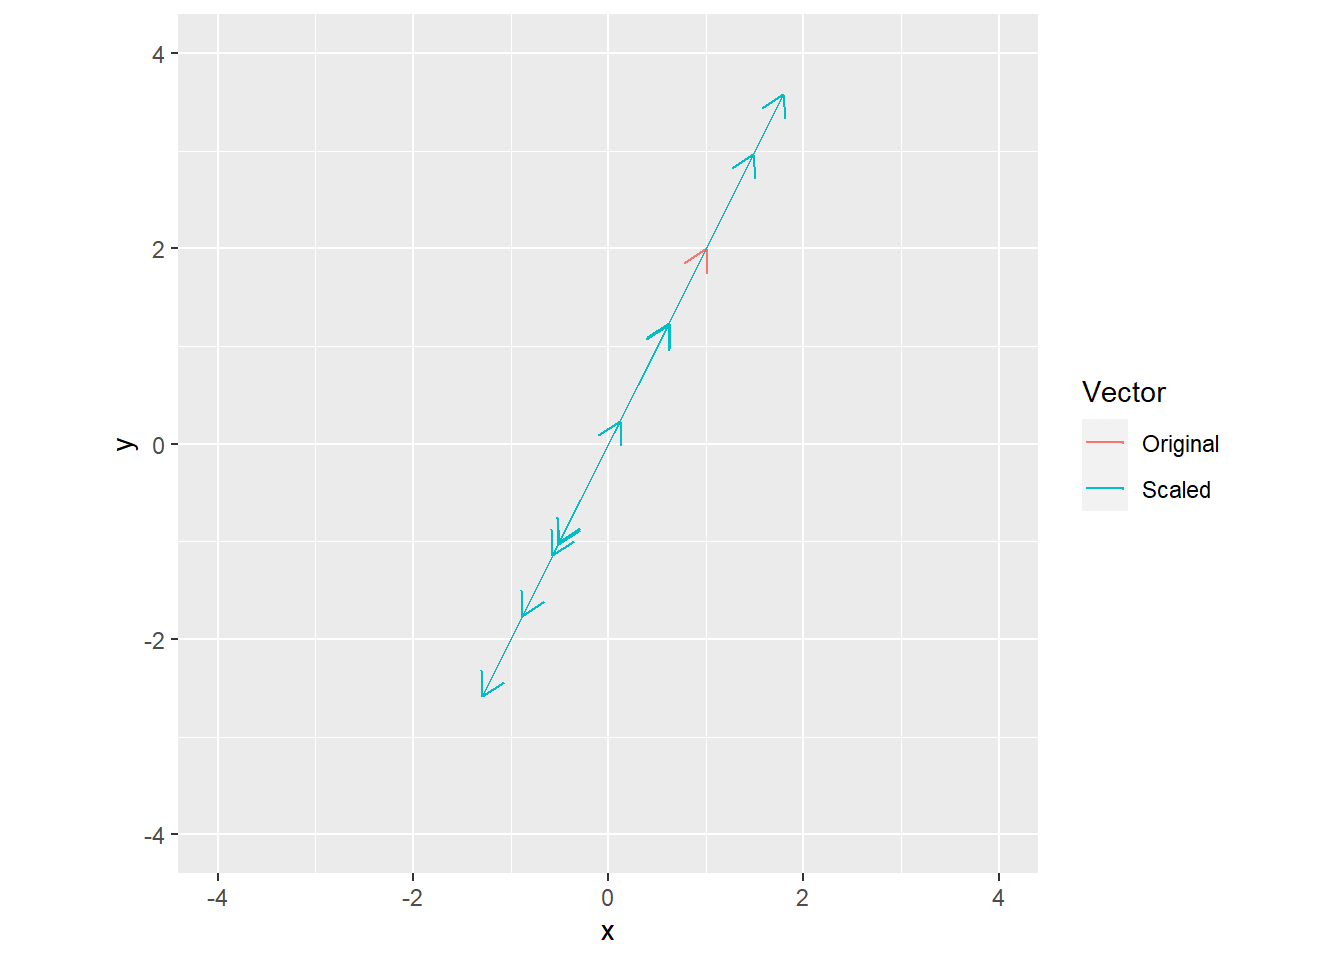
\includegraphics{cohen-linear-algebra_files/figure-latex/e02-1-1.pdf}

\hypertarget{chapter-3-1}{%
\section*{Chapter 3}\label{chapter-3-1}}
\addcontentsline{toc}{section}{Chapter 3}

\hypertarget{exercise-1}{%
\subsection*{Exercise 1}\label{exercise-1}}
\addcontentsline{toc}{subsection}{Exercise 1}

\begin{Shaded}
\begin{Highlighting}[]
\NormalTok{v1 \textless{}{-}}\StringTok{ }\KeywordTok{c}\NormalTok{(}\DecValTok{1}\NormalTok{, }\DecValTok{2}\NormalTok{, }\DecValTok{3}\NormalTok{, }\DecValTok{4}\NormalTok{, }\DecValTok{5}\NormalTok{)}
\NormalTok{v2 \textless{}{-}}\StringTok{ }\KeywordTok{c}\NormalTok{(}\DecValTok{2}\NormalTok{, }\DecValTok{3}\NormalTok{, }\DecValTok{4}\NormalTok{, }\DecValTok{5}\NormalTok{, }\DecValTok{6}\NormalTok{)}
\NormalTok{v3 \textless{}{-}}\StringTok{ }\KeywordTok{c}\NormalTok{(}\DecValTok{3}\NormalTok{, }\DecValTok{4}\NormalTok{, }\DecValTok{5}\NormalTok{, }\DecValTok{6}\NormalTok{, }\DecValTok{7}\NormalTok{)}
\NormalTok{w \textless{}{-}}\StringTok{ }\KeywordTok{c}\NormalTok{(}\OperatorTok{{-}}\DecValTok{1}\NormalTok{, }\DecValTok{3}\NormalTok{, }\DecValTok{2}\NormalTok{)}
\NormalTok{result \textless{}{-}}\StringTok{ }\NormalTok{v1 }\OperatorTok{*}\StringTok{ }\NormalTok{w[}\DecValTok{1}\NormalTok{] }\OperatorTok{+}\StringTok{ }\NormalTok{v2 }\OperatorTok{*}\StringTok{ }\NormalTok{w[}\DecValTok{2}\NormalTok{] }\OperatorTok{+}\StringTok{ }\NormalTok{v3}\OperatorTok{*}\StringTok{ }\NormalTok{w[}\DecValTok{3}\NormalTok{]}
\end{Highlighting}
\end{Shaded}

\hypertarget{exercise-2}{%
\subsection*{Exercise 2}\label{exercise-2}}
\addcontentsline{toc}{subsection}{Exercise 2}

\begin{Shaded}
\begin{Highlighting}[]
\NormalTok{v \textless{}{-}}\StringTok{ }\KeywordTok{c}\NormalTok{(}\DecValTok{7}\NormalTok{, }\DecValTok{4}\NormalTok{, }\DecValTok{{-}5}\NormalTok{, }\DecValTok{8}\NormalTok{, }\DecValTok{3}\NormalTok{)}
\NormalTok{o \textless{}{-}}\StringTok{ }\KeywordTok{rep}\NormalTok{(}\DecValTok{1}\NormalTok{, }\KeywordTok{length}\NormalTok{(v))}
\NormalTok{ave \textless{}{-}}\StringTok{ }\NormalTok{pracma}\OperatorTok{::}\KeywordTok{dot}\NormalTok{(v, o) }\OperatorTok{/}\StringTok{ }\KeywordTok{length}\NormalTok{(v)}
\end{Highlighting}
\end{Shaded}

\hypertarget{exercise-3}{%
\subsection*{Exercise 3}\label{exercise-3}}
\addcontentsline{toc}{subsection}{Exercise 3}

\begin{Shaded}
\begin{Highlighting}[]
\NormalTok{v \textless{}{-}}\StringTok{ }\KeywordTok{c}\NormalTok{(}\DecValTok{7}\NormalTok{, }\DecValTok{4}\NormalTok{, }\DecValTok{{-}5}\NormalTok{, }\DecValTok{8}\NormalTok{, }\DecValTok{3}\NormalTok{)}
\NormalTok{w \textless{}{-}}\StringTok{ }\KeywordTok{runif}\NormalTok{(}\KeywordTok{length}\NormalTok{(v))}
\NormalTok{wAve \textless{}{-}}\StringTok{ }\NormalTok{pracma}\OperatorTok{::}\KeywordTok{dot}\NormalTok{(v, w }\OperatorTok{/}\StringTok{ }\KeywordTok{sum}\NormalTok{(w))}
\end{Highlighting}
\end{Shaded}

\hypertarget{chapter-5-1}{%
\section*{Chapter 5}\label{chapter-5-1}}
\addcontentsline{toc}{section}{Chapter 5}

\hypertarget{exercise-1-1}{%
\subsection*{Exercise 1}\label{exercise-1-1}}
\addcontentsline{toc}{subsection}{Exercise 1}

\begin{Shaded}
\begin{Highlighting}[]
\NormalTok{A \textless{}{-}}\StringTok{ }\KeywordTok{matrix}\NormalTok{(}\KeywordTok{runif}\NormalTok{(}\DataTypeTok{n=}\DecValTok{4}\OperatorTok{*}\DecValTok{2}\NormalTok{), }\DataTypeTok{nrow=}\DecValTok{4}\NormalTok{, }\DataTypeTok{ncol=}\DecValTok{2}\NormalTok{)}
\NormalTok{B \textless{}{-}}\StringTok{ }\KeywordTok{matrix}\NormalTok{(}\KeywordTok{runif}\NormalTok{(}\DataTypeTok{n=}\DecValTok{4}\OperatorTok{*}\DecValTok{2}\NormalTok{), }\DataTypeTok{nrow=}\DecValTok{4}\NormalTok{, }\DataTypeTok{ncol=}\DecValTok{2}\NormalTok{)}
\NormalTok{C \textless{}{-}}\StringTok{ }\KeywordTok{matrix}\NormalTok{(}\OtherTok{NA}\NormalTok{, }\DataTypeTok{nrow=}\DecValTok{2}\NormalTok{, }\DataTypeTok{ncol=}\DecValTok{2}\NormalTok{)}
\ControlFlowTok{for}\NormalTok{(coli }\ControlFlowTok{in} \DecValTok{1}\OperatorTok{:}\DecValTok{2}\NormalTok{)\{}
  \ControlFlowTok{for}\NormalTok{(colj }\ControlFlowTok{in} \DecValTok{1}\OperatorTok{:}\DecValTok{2}\NormalTok{)\{}
\NormalTok{    C[coli, colj] \textless{}{-}}\StringTok{ }\NormalTok{pracma}\OperatorTok{::}\KeywordTok{dot}\NormalTok{(A[, coli], B[, colj])}
\NormalTok{  \}}
\NormalTok{\}}
\end{Highlighting}
\end{Shaded}

\hypertarget{exercise-2-1}{%
\subsection*{Exercise 2}\label{exercise-2-1}}
\addcontentsline{toc}{subsection}{Exercise 2}

\begin{Shaded}
\begin{Highlighting}[]
\NormalTok{A \textless{}{-}}\StringTok{ }\KeywordTok{matrix}\NormalTok{(}\KeywordTok{runif}\NormalTok{(}\DataTypeTok{n=}\DecValTok{4}\OperatorTok{*}\DecValTok{4}\NormalTok{), }\DataTypeTok{nrow=}\DecValTok{4}\NormalTok{, }\DataTypeTok{ncol=}\DecValTok{4}\NormalTok{)}
\NormalTok{Al \textless{}{-}}\StringTok{ }\NormalTok{pracma}\OperatorTok{::}\KeywordTok{tril}\NormalTok{(A)}
\NormalTok{S \textless{}{-}}\StringTok{ }\NormalTok{Al }\OperatorTok{+}\StringTok{ }\KeywordTok{t}\NormalTok{(Al)}
\end{Highlighting}
\end{Shaded}

\hypertarget{exercise-3-1}{%
\subsection*{Exercise 3}\label{exercise-3-1}}
\addcontentsline{toc}{subsection}{Exercise 3}

\begin{Shaded}
\begin{Highlighting}[]
\NormalTok{D \textless{}{-}}\StringTok{ }\KeywordTok{matrix}\NormalTok{(}\DecValTok{0}\NormalTok{, }\DataTypeTok{nrow=}\DecValTok{4}\NormalTok{, }\DataTypeTok{ncol=}\DecValTok{8}\NormalTok{)}
\ControlFlowTok{for}\NormalTok{(d }\ControlFlowTok{in} \DecValTok{1}\OperatorTok{:}\KeywordTok{min}\NormalTok{(}\KeywordTok{dim}\NormalTok{(D)))\{}
\NormalTok{  D[d, d] \textless{}{-}}\StringTok{ }\NormalTok{d}
\NormalTok{\}}

\CommentTok{\# or}
\NormalTok{D \textless{}{-}}\StringTok{ }\KeywordTok{diag}\NormalTok{(}\DecValTok{1}\OperatorTok{:}\DecValTok{4}\NormalTok{, }\DataTypeTok{nrow=}\DecValTok{4}\NormalTok{, }\DataTypeTok{ncol=}\DecValTok{8}\NormalTok{)}
\end{Highlighting}
\end{Shaded}

\hypertarget{chapter-6-1}{%
\section*{Chapter 6}\label{chapter-6-1}}
\addcontentsline{toc}{section}{Chapter 6}

\hypertarget{exercise-1-2}{%
\subsection*{Exercise 1}\label{exercise-1-2}}
\addcontentsline{toc}{subsection}{Exercise 1}

\begin{Shaded}
\begin{Highlighting}[]
\NormalTok{A \textless{}{-}}\StringTok{ }\KeywordTok{matrix}\NormalTok{(}\KeywordTok{runif}\NormalTok{(}\DataTypeTok{n=}\DecValTok{2}\OperatorTok{*}\DecValTok{4}\NormalTok{), }\DataTypeTok{nrow=}\DecValTok{2}\NormalTok{, }\DataTypeTok{ncol=}\DecValTok{4}\NormalTok{)}
\NormalTok{B \textless{}{-}}\StringTok{ }\KeywordTok{matrix}\NormalTok{(}\KeywordTok{runif}\NormalTok{(}\DataTypeTok{n=}\DecValTok{4}\OperatorTok{*}\DecValTok{3}\NormalTok{), }\DataTypeTok{nrow=}\DecValTok{4}\NormalTok{, }\DataTypeTok{ncol=}\DecValTok{3}\NormalTok{)}
\NormalTok{C1 \textless{}{-}}\StringTok{ }\KeywordTok{matrix}\NormalTok{(}\DecValTok{0}\NormalTok{, }\DataTypeTok{nrow=}\DecValTok{2}\NormalTok{, }\DataTypeTok{ncol=}\DecValTok{3}\NormalTok{)}
\ControlFlowTok{for}\NormalTok{(i }\ControlFlowTok{in} \DecValTok{1}\OperatorTok{:}\DecValTok{4}\NormalTok{)\{}
\NormalTok{  C1 \textless{}{-}}\StringTok{ }\NormalTok{C1 }\OperatorTok{+}\StringTok{ }\KeywordTok{outer}\NormalTok{(A[, i], B[i, ])}
\NormalTok{\}}
\NormalTok{C1 }\OperatorTok{{-}}\StringTok{ }\NormalTok{A }\OperatorTok{\%*\%}\StringTok{ }\NormalTok{B}
\end{Highlighting}
\end{Shaded}

\begin{verbatim}
##      [,1] [,2] [,3]
## [1,]    0    0    0
## [2,]    0    0    0
\end{verbatim}

\hypertarget{exercise-2-2}{%
\subsection*{Exercise 2}\label{exercise-2-2}}
\addcontentsline{toc}{subsection}{Exercise 2}

\begin{Shaded}
\begin{Highlighting}[]
\NormalTok{D \textless{}{-}}\StringTok{ }\KeywordTok{diag}\NormalTok{(}\DecValTok{1}\OperatorTok{:}\DecValTok{4}\NormalTok{)}
\NormalTok{A \textless{}{-}}\StringTok{ }\KeywordTok{matrix}\NormalTok{(}\KeywordTok{runif}\NormalTok{(}\DataTypeTok{n=}\DecValTok{4}\OperatorTok{*}\DecValTok{4}\NormalTok{), }\DataTypeTok{nrow=}\DecValTok{4}\NormalTok{, }\DataTypeTok{ncol=}\DecValTok{4}\NormalTok{)}
\NormalTok{C1 \textless{}{-}}\StringTok{ }\NormalTok{D }\OperatorTok{*}\StringTok{ }\NormalTok{A}
\NormalTok{C2 \textless{}{-}}\StringTok{ }\NormalTok{D }\OperatorTok{\%*\%}\StringTok{ }\NormalTok{A}
\KeywordTok{print}\NormalTok{(}\KeywordTok{diag}\NormalTok{(C1))}
\end{Highlighting}
\end{Shaded}

\begin{verbatim}
## [1] 0.1711260 0.3780008 0.3330304 2.2317351
\end{verbatim}

\begin{Shaded}
\begin{Highlighting}[]
\KeywordTok{print}\NormalTok{(}\KeywordTok{diag}\NormalTok{(C2))}
\end{Highlighting}
\end{Shaded}

\begin{verbatim}
## [1] 0.1711260 0.3780008 0.3330304 2.2317351
\end{verbatim}

\hypertarget{exercise-3-2}{%
\subsection*{Exercise 3}\label{exercise-3-2}}
\addcontentsline{toc}{subsection}{Exercise 3}

\begin{Shaded}
\begin{Highlighting}[]
\NormalTok{A \textless{}{-}}\StringTok{ }\KeywordTok{diag}\NormalTok{(}\KeywordTok{runif}\NormalTok{(}\DecValTok{3}\NormalTok{))}
\NormalTok{C1 \textless{}{-}}\StringTok{ }\NormalTok{(}\KeywordTok{t}\NormalTok{(A) }\OperatorTok{+}\StringTok{ }\NormalTok{A) }\OperatorTok{/}\StringTok{ }\DecValTok{2}
\NormalTok{C2 \textless{}{-}}\StringTok{ }\KeywordTok{t}\NormalTok{(A) }\OperatorTok{\%*\%}\StringTok{ }\NormalTok{A}
\NormalTok{C1 }\OperatorTok{{-}}\StringTok{ }\KeywordTok{sqrt}\NormalTok{(C2)}
\end{Highlighting}
\end{Shaded}

\begin{verbatim}
##      [,1] [,2] [,3]
## [1,]    0    0    0
## [2,]    0    0    0
## [3,]    0    0    0
\end{verbatim}

\hypertarget{exercise-4}{%
\subsection*{Exercise 4}\label{exercise-4}}
\addcontentsline{toc}{subsection}{Exercise 4}

Note that \texttt{norm()} requires a matrix as an input, therefore, we convert an atomic vector to a matrix for the norm computation.

\begin{Shaded}
\begin{Highlighting}[]
\NormalTok{m \textless{}{-}}\StringTok{ }\DecValTok{5}
\NormalTok{A \textless{}{-}}\StringTok{ }\KeywordTok{matrix}\NormalTok{(}\KeywordTok{runif}\NormalTok{(}\DataTypeTok{n=}\NormalTok{m}\OperatorTok{*}\NormalTok{m), }\DataTypeTok{nrow=}\NormalTok{m, }\DataTypeTok{ncol=}\NormalTok{m)}
\NormalTok{v \textless{}{-}}\StringTok{ }\KeywordTok{runif}\NormalTok{(}\DataTypeTok{n=}\NormalTok{m)}
\NormalTok{LHS \textless{}{-}}\StringTok{ }\KeywordTok{norm}\NormalTok{(A }\OperatorTok{\%*\%}\StringTok{ }\NormalTok{v, }\DataTypeTok{type =} \StringTok{"F"}\NormalTok{)}
\NormalTok{RHS \textless{}{-}}\StringTok{ }\KeywordTok{norm}\NormalTok{(A, }\DataTypeTok{type =} \StringTok{"F"}\NormalTok{) }\OperatorTok{*}\StringTok{ }\KeywordTok{norm}\NormalTok{(}\KeywordTok{matrix}\NormalTok{(v), }\DataTypeTok{type=}\StringTok{"F"}\NormalTok{)}
\NormalTok{RHS }\OperatorTok{{-}}\StringTok{ }\NormalTok{LHS }\CommentTok{\# should always be positive}
\end{Highlighting}
\end{Shaded}

\begin{verbatim}
## [1] 0.844411
\end{verbatim}

\hypertarget{chapter-7-1}{%
\section*{Chapter 7}\label{chapter-7-1}}
\addcontentsline{toc}{section}{Chapter 7}

\hypertarget{exercise-1-3}{%
\subsection*{Exercise 1}\label{exercise-1-3}}
\addcontentsline{toc}{subsection}{Exercise 1}

\begin{Shaded}
\begin{Highlighting}[]
\NormalTok{A \textless{}{-}}\StringTok{ }\KeywordTok{matrix}\NormalTok{(}\KeywordTok{runif}\NormalTok{(}\DataTypeTok{n=}\DecValTok{9}\OperatorTok{*}\DecValTok{2}\NormalTok{), }\DataTypeTok{nrow=}\DecValTok{9}\NormalTok{, }\DataTypeTok{ncol=}\DecValTok{2}\NormalTok{)}
\NormalTok{B \textless{}{-}}\StringTok{ }\KeywordTok{matrix}\NormalTok{(}\KeywordTok{runif}\NormalTok{(}\DataTypeTok{n=}\DecValTok{2}\OperatorTok{*}\DecValTok{16}\NormalTok{), }\DataTypeTok{nrow=}\DecValTok{2}\NormalTok{, }\DataTypeTok{ncol=}\DecValTok{16}\NormalTok{)}
\NormalTok{C \textless{}{-}}\StringTok{ }\NormalTok{A }\OperatorTok{\%*\%}\StringTok{ }\NormalTok{B}
\end{Highlighting}
\end{Shaded}

\hypertarget{exercise-2-3}{%
\subsection*{Exercise 2}\label{exercise-2-3}}
\addcontentsline{toc}{subsection}{Exercise 2}

\begin{Shaded}
\begin{Highlighting}[]
\NormalTok{Z \textless{}{-}}\StringTok{ }\KeywordTok{matrix}\NormalTok{(}\DecValTok{0}\NormalTok{, }\DataTypeTok{nrow=}\DecValTok{5}\NormalTok{, }\DataTypeTok{ncol=}\DecValTok{5}\NormalTok{)}
\NormalTok{N \textless{}{-}}\StringTok{ }\KeywordTok{matrix}\NormalTok{(}\KeywordTok{runif}\NormalTok{(}\DecValTok{5} \OperatorTok{*}\StringTok{ }\DecValTok{5}\NormalTok{), }\DataTypeTok{nrow=}\DecValTok{5}\NormalTok{, }\DataTypeTok{ncol=}\DecValTok{5}\NormalTok{)}
\NormalTok{ZN \textless{}{-}}\StringTok{  }\NormalTok{Z }\OperatorTok{+}\StringTok{ }\NormalTok{N }\OperatorTok{*}\StringTok{ }\NormalTok{.Machine}\OperatorTok{$}\NormalTok{double.eps }\OperatorTok{*}\StringTok{ }\FloatTok{1e{-}307}
\KeywordTok{print}\NormalTok{(pracma}\OperatorTok{::}\KeywordTok{Rank}\NormalTok{(Z))}
\end{Highlighting}
\end{Shaded}

\begin{verbatim}
## [1] 0
\end{verbatim}

\begin{Shaded}
\begin{Highlighting}[]
\KeywordTok{print}\NormalTok{(pracma}\OperatorTok{::}\KeywordTok{Rank}\NormalTok{(ZN))}
\end{Highlighting}
\end{Shaded}

\begin{verbatim}
## Warning in pracma::Rank(ZN): Rank calculation may be problematic.
\end{verbatim}

\begin{verbatim}
## [1] 4
\end{verbatim}

\begin{Shaded}
\begin{Highlighting}[]
\KeywordTok{print}\NormalTok{(}\KeywordTok{norm}\NormalTok{(ZN, }\DataTypeTok{type =} \StringTok{"F"}\NormalTok{))}
\end{Highlighting}
\end{Shaded}

\begin{verbatim}
## [1] 6.916919e-323
\end{verbatim}

\hypertarget{chapter-8-1}{%
\section*{Chapter 8}\label{chapter-8-1}}
\addcontentsline{toc}{section}{Chapter 8}

\hypertarget{exercise-1-4}{%
\subsection*{Exercise 1}\label{exercise-1-4}}
\addcontentsline{toc}{subsection}{Exercise 1}

\begin{Shaded}
\begin{Highlighting}[]
\NormalTok{A \textless{}{-}}\StringTok{ }\KeywordTok{matrix}\NormalTok{(}\KeywordTok{runif}\NormalTok{(}\DataTypeTok{n=}\DecValTok{4}\OperatorTok{*}\DecValTok{3}\NormalTok{), }\DataTypeTok{nrow=}\DecValTok{4}\NormalTok{, }\DataTypeTok{ncol=}\DecValTok{3}\NormalTok{) }\OperatorTok{\%*\%}\StringTok{ }\KeywordTok{matrix}\NormalTok{(}\KeywordTok{runif}\NormalTok{(}\DataTypeTok{n=}\DecValTok{3}\OperatorTok{*}\DecValTok{4}\NormalTok{), }\DataTypeTok{nrow=}\DecValTok{3}\NormalTok{, }\DataTypeTok{ncol=}\DecValTok{4}\NormalTok{)}
\NormalTok{B \textless{}{-}}\StringTok{ }\KeywordTok{matrix}\NormalTok{(}\KeywordTok{runif}\NormalTok{(}\DataTypeTok{n=}\DecValTok{4}\OperatorTok{*}\DecValTok{3}\NormalTok{), }\DataTypeTok{nrow=}\DecValTok{4}\NormalTok{, }\DataTypeTok{ncol=}\DecValTok{3}\NormalTok{) }\OperatorTok{\%*\%}\StringTok{ }\KeywordTok{matrix}\NormalTok{(}\KeywordTok{runif}\NormalTok{(}\DataTypeTok{n=}\DecValTok{3}\OperatorTok{*}\DecValTok{4}\NormalTok{), }\DataTypeTok{nrow=}\DecValTok{3}\NormalTok{, }\DataTypeTok{ncol=}\DecValTok{4}\NormalTok{)}
\NormalTok{n \textless{}{-}}\StringTok{ }\NormalTok{pracma}\OperatorTok{::}\KeywordTok{nullspace}\NormalTok{(A)}
\KeywordTok{print}\NormalTok{(B }\OperatorTok{\%*\%}\StringTok{ }\NormalTok{A }\OperatorTok{\%*\%}\StringTok{ }\NormalTok{n) }\CommentTok{\# zeros vector}
\end{Highlighting}
\end{Shaded}

\begin{verbatim}
##              [,1]
## [1,] 2.185752e-16
## [2,] 9.020562e-17
## [3,] 4.336809e-17
## [4,] 7.285839e-17
\end{verbatim}

\begin{Shaded}
\begin{Highlighting}[]
\KeywordTok{print}\NormalTok{(A }\OperatorTok{\%*\%}\StringTok{ }\NormalTok{B }\OperatorTok{\%*\%}\StringTok{ }\NormalTok{n) }\CommentTok{\# not zeros vector}
\end{Highlighting}
\end{Shaded}

\begin{verbatim}
##             [,1]
## [1,] -0.15753980
## [2,] -0.11473846
## [3,] -0.07792846
## [4,] -0.08309196
\end{verbatim}

\hypertarget{exercise-2-4}{%
\subsection*{Exercise 2}\label{exercise-2-4}}
\addcontentsline{toc}{subsection}{Exercise 2}

\begin{Shaded}
\begin{Highlighting}[]
\NormalTok{A \textless{}{-}}\StringTok{ }\KeywordTok{matrix}\NormalTok{(}\KeywordTok{runif}\NormalTok{(}\DataTypeTok{n=}\DecValTok{16}\OperatorTok{*}\DecValTok{9}\NormalTok{), }\DataTypeTok{nrow=}\DecValTok{16}\NormalTok{, }\DataTypeTok{ncol=}\DecValTok{9}\NormalTok{) }\OperatorTok{\%*\%}\StringTok{ }\KeywordTok{matrix}\NormalTok{(}\KeywordTok{runif}\NormalTok{(}\DataTypeTok{n=}\DecValTok{9}\OperatorTok{*}\DecValTok{11}\NormalTok{), }\DataTypeTok{nrow=}\DecValTok{9}\NormalTok{, }\DataTypeTok{ncol=}\DecValTok{11}\NormalTok{)}
\NormalTok{rn \textless{}{-}}\StringTok{ }\NormalTok{pracma}\OperatorTok{::}\KeywordTok{nullspace}\NormalTok{(A)}
\NormalTok{ln \textless{}{-}}\StringTok{ }\NormalTok{pracma}\OperatorTok{::}\KeywordTok{nullspace}\NormalTok{(}\KeywordTok{t}\NormalTok{(A))}
\NormalTok{r \textless{}{-}}\StringTok{ }\NormalTok{pracma}\OperatorTok{::}\KeywordTok{Rank}\NormalTok{(A)}
\KeywordTok{print}\NormalTok{(}\KeywordTok{ncol}\NormalTok{(rn) }\OperatorTok{+}\StringTok{ }\NormalTok{r)}
\end{Highlighting}
\end{Shaded}

\begin{verbatim}
## [1] 11
\end{verbatim}

\begin{Shaded}
\begin{Highlighting}[]
\KeywordTok{print}\NormalTok{(}\KeywordTok{ncol}\NormalTok{(ln) }\OperatorTok{+}\StringTok{ }\NormalTok{r)}
\end{Highlighting}
\end{Shaded}

\begin{verbatim}
## [1] 16
\end{verbatim}

\hypertarget{chapter-9-1}{%
\section*{Chapter 9}\label{chapter-9-1}}
\addcontentsline{toc}{section}{Chapter 9}

\hypertarget{exercise-1-5}{%
\subsection*{Exercise 1}\label{exercise-1-5}}
\addcontentsline{toc}{subsection}{Exercise 1}

Base R does not implement Hermitian transpose directly and you are advised to compute it via \texttt{Conj(t(A))}, see \emph{Notes} for {[}t(){]}(\url{https://stat.ethz.ch/R-manual/R-devel/library/base/html/t.html} function.

\begin{Shaded}
\begin{Highlighting}[]
\NormalTok{U \textless{}{-}}\StringTok{ }\FloatTok{0.5} \OperatorTok{*}\StringTok{ }\KeywordTok{matrix}\NormalTok{(}\KeywordTok{c}\NormalTok{(}\DecValTok{1}\OperatorTok{+}\NormalTok{1i, }\DecValTok{1}\OperatorTok{{-}}\NormalTok{1i, }\DecValTok{1}\OperatorTok{{-}}\NormalTok{1i, }\DecValTok{1}\OperatorTok{+}\NormalTok{1i), }\DataTypeTok{nrow=}\DecValTok{2}\NormalTok{, }\DataTypeTok{ncol=}\DecValTok{2}\NormalTok{)}
\KeywordTok{print}\NormalTok{(U }\OperatorTok{\%*\%}\StringTok{ }\KeywordTok{Conj}\NormalTok{(}\KeywordTok{t}\NormalTok{(U))) }\CommentTok{\# Hermitian}
\end{Highlighting}
\end{Shaded}

\begin{verbatim}
##      [,1] [,2]
## [1,] 1+0i 0+0i
## [2,] 0+0i 1+0i
\end{verbatim}

\begin{Shaded}
\begin{Highlighting}[]
\KeywordTok{print}\NormalTok{(U }\OperatorTok{\%*\%}\StringTok{ }\KeywordTok{t}\NormalTok{(U)) }\CommentTok{\# not Hermitian}
\end{Highlighting}
\end{Shaded}

\begin{verbatim}
##      [,1] [,2]
## [1,] 0+0i 1+0i
## [2,] 1+0i 0+0i
\end{verbatim}

\hypertarget{exercise-2-5}{%
\subsection*{Exercise 2}\label{exercise-2-5}}
\addcontentsline{toc}{subsection}{Exercise 2}

In contrast to Matlab, a complex matrix
\href{https://stat.ethz.ch/R-manual/R-devel/library/base/html/isSymmetric.html}{isSymmetric()} only if it is Hermitian.

\begin{Shaded}
\begin{Highlighting}[]
\NormalTok{r \textless{}{-}}\StringTok{ }\KeywordTok{matrix}\NormalTok{(}\KeywordTok{runif}\NormalTok{(}\DataTypeTok{n=}\DecValTok{3}\OperatorTok{*}\DecValTok{3}\NormalTok{), }\DataTypeTok{nrow=}\DecValTok{3}\NormalTok{, }\DataTypeTok{ncol=}\DecValTok{3}\NormalTok{)}
\NormalTok{im \textless{}{-}}\StringTok{ }\KeywordTok{matrix}\NormalTok{(}\KeywordTok{runif}\NormalTok{(}\DataTypeTok{n=}\DecValTok{3}\OperatorTok{*}\DecValTok{3}\NormalTok{), }\DataTypeTok{nrow=}\DecValTok{3}\NormalTok{, }\DataTypeTok{ncol=}\DecValTok{3}\NormalTok{)}
\NormalTok{A \textless{}{-}}\StringTok{ }\NormalTok{r }\OperatorTok{+}\StringTok{ }\NormalTok{im }\OperatorTok{*}\StringTok{ }\NormalTok{1i}
\NormalTok{A1 \textless{}{-}}\StringTok{ }\NormalTok{A }\OperatorTok{+}\StringTok{ }\KeywordTok{Conj}\NormalTok{(}\KeywordTok{t}\NormalTok{(A))}
\NormalTok{A2 \textless{}{-}}\StringTok{ }\NormalTok{A }\OperatorTok{\%*\%}\StringTok{ }\KeywordTok{Conj}\NormalTok{(}\KeywordTok{t}\NormalTok{(A))}
\KeywordTok{isSymmetric}\NormalTok{(A1)}
\end{Highlighting}
\end{Shaded}

\begin{verbatim}
## [1] TRUE
\end{verbatim}

\begin{Shaded}
\begin{Highlighting}[]
\KeywordTok{isSymmetric}\NormalTok{(A2)}
\end{Highlighting}
\end{Shaded}

\begin{verbatim}
## [1] TRUE
\end{verbatim}

\hypertarget{chapter-10-1}{%
\section*{Chapter 10}\label{chapter-10-1}}
\addcontentsline{toc}{section}{Chapter 10}

\hypertarget{exercise-1-6}{%
\subsection*{Exercise 1}\label{exercise-1-6}}
\addcontentsline{toc}{subsection}{Exercise 1}

\begin{Shaded}
\begin{Highlighting}[]
\NormalTok{A \textless{}{-}}\StringTok{ }\KeywordTok{matrix}\NormalTok{(}\KeywordTok{c}\NormalTok{(}\DecValTok{2}\NormalTok{, }\DecValTok{0}\NormalTok{, }\DecValTok{{-}3}\NormalTok{, }\DecValTok{3}\NormalTok{, }\DecValTok{1}\NormalTok{, }\DecValTok{4}\NormalTok{, }\DecValTok{1}\NormalTok{, }\DecValTok{0}\NormalTok{, }\DecValTok{{-}1}\NormalTok{), }\DataTypeTok{nrow=}\DecValTok{3}\NormalTok{, }\DataTypeTok{byrow=}\OtherTok{TRUE}\NormalTok{)}
\NormalTok{x \textless{}{-}}\StringTok{ }\KeywordTok{matrix}\NormalTok{(}\KeywordTok{c}\NormalTok{(}\DecValTok{2}\NormalTok{, }\DecValTok{3}\NormalTok{, }\DecValTok{4}\NormalTok{), }\DataTypeTok{ncol=}\DecValTok{1}\NormalTok{)}
\NormalTok{b \textless{}{-}}\StringTok{ }\NormalTok{A }\OperatorTok{\%*\%}\StringTok{ }\NormalTok{x}
\end{Highlighting}
\end{Shaded}

\hypertarget{exercise-2-6}{%
\subsection*{Exercise 2}\label{exercise-2-6}}
\addcontentsline{toc}{subsection}{Exercise 2}

\begin{Shaded}
\begin{Highlighting}[]
\NormalTok{A \textless{}{-}}\StringTok{ }\KeywordTok{matrix}\NormalTok{(}\KeywordTok{runif}\NormalTok{(}\DataTypeTok{n=}\DecValTok{3}\OperatorTok{*}\DecValTok{6}\NormalTok{), }\DataTypeTok{nrow=}\DecValTok{3}\NormalTok{, }\DataTypeTok{ncol=}\DecValTok{6}\NormalTok{)}
\NormalTok{pracma}\OperatorTok{::}\KeywordTok{rref}\NormalTok{(A)}
\end{Highlighting}
\end{Shaded}

\begin{verbatim}
##      [,1] [,2] [,3]        [,4]      [,5]       [,6]
## [1,]    1    0    0  0.76056444 0.6611005 -0.5022564
## [2,]    0    1    0  0.91003537 0.4225203  0.8952120
## [3,]    0    0    1 -0.02330263 0.2688984  0.8249581
\end{verbatim}

\hypertarget{chapter-11-1}{%
\section*{Chapter 11}\label{chapter-11-1}}
\addcontentsline{toc}{section}{Chapter 11}

\hypertarget{exercise-1-7}{%
\subsection*{Exercise 1}\label{exercise-1-7}}
\addcontentsline{toc}{subsection}{Exercise 1}

\begin{Shaded}
\begin{Highlighting}[]
\NormalTok{A \textless{}{-}}\StringTok{ }\KeywordTok{matrix}\NormalTok{(}\KeywordTok{sample}\NormalTok{(}\DecValTok{0}\OperatorTok{:}\DecValTok{10}\NormalTok{, }\DataTypeTok{size=}\DecValTok{4}\OperatorTok{*}\DecValTok{4}\NormalTok{, }\DataTypeTok{replace=}\OtherTok{TRUE}\NormalTok{), }\DataTypeTok{nrow=}\DecValTok{4}\NormalTok{, }\DataTypeTok{ncol=}\DecValTok{4}\NormalTok{)}
\NormalTok{b \textless{}{-}}\StringTok{ }\KeywordTok{sample}\NormalTok{(}\OperatorTok{{-}}\DecValTok{10}\OperatorTok{:{-}}\DecValTok{1}\NormalTok{, }\DataTypeTok{size=}\DecValTok{1}\NormalTok{)}
\KeywordTok{print}\NormalTok{(}\KeywordTok{det}\NormalTok{(b }\OperatorTok{*}\StringTok{ }\NormalTok{A))}
\end{Highlighting}
\end{Shaded}

\begin{verbatim}
## [1] 6880000
\end{verbatim}

\begin{Shaded}
\begin{Highlighting}[]
\KeywordTok{print}\NormalTok{(b}\OperatorTok{\^{}}\KeywordTok{nrow}\NormalTok{(A) }\OperatorTok{*}\StringTok{ }\KeywordTok{det}\NormalTok{(A))}
\end{Highlighting}
\end{Shaded}

\begin{verbatim}
## [1] 6880000
\end{verbatim}

\hypertarget{exercise-2-7}{%
\subsection*{Exercise 2}\label{exercise-2-7}}
\addcontentsline{toc}{subsection}{Exercise 2}

\begin{Shaded}
\begin{Highlighting}[]
\KeywordTok{library}\NormalTok{(ggplot2)}

\NormalTok{ns \textless{}{-}}\StringTok{ }\DecValTok{3}\OperatorTok{:}\DecValTok{30}
\NormalTok{iters \textless{}{-}}\StringTok{ }\DecValTok{100}
\NormalTok{dets \textless{}{-}}\StringTok{ }\KeywordTok{matrix}\NormalTok{(}\DecValTok{0}\NormalTok{, }\DataTypeTok{nrow=}\KeywordTok{length}\NormalTok{(ns), }\DataTypeTok{ncol =}\NormalTok{ iters)}

\ControlFlowTok{for}\NormalTok{(ni }\ControlFlowTok{in} \DecValTok{1}\OperatorTok{:}\KeywordTok{length}\NormalTok{(ns))\{}
  \ControlFlowTok{for}\NormalTok{(it }\ControlFlowTok{in} \DecValTok{1}\OperatorTok{:}\NormalTok{iters)\{}
\NormalTok{    A \textless{}{-}}\StringTok{ }\KeywordTok{matrix}\NormalTok{(}\KeywordTok{rnorm}\NormalTok{(}\DataTypeTok{n=}\NormalTok{ns[ni]}\OperatorTok{\^{}}\DecValTok{2}\NormalTok{), }\DataTypeTok{nrow=}\NormalTok{ns[ni], }\DataTypeTok{ncol=}\NormalTok{ns[ni]) }\CommentTok{\# step 1}
\NormalTok{    A[, }\DecValTok{1}\NormalTok{] \textless{}{-}}\StringTok{ }\NormalTok{A[, }\DecValTok{2}\NormalTok{]  }\CommentTok{\# step 2  }
\NormalTok{    dets[ni, it] \textless{}{-}}\StringTok{ }\KeywordTok{abs}\NormalTok{(}\KeywordTok{det}\NormalTok{(A)) }\CommentTok{\# step 3}
\NormalTok{  \}}
\NormalTok{\}}

\NormalTok{dets\_summary \textless{}{-}}\StringTok{ }
\StringTok{  }\KeywordTok{data.frame}\NormalTok{(}\DataTypeTok{MatrixSize =}\NormalTok{ ns,}
             \DataTypeTok{LogDeterminant =} \KeywordTok{log}\NormalTok{(}\KeywordTok{apply}\NormalTok{(dets, }\DataTypeTok{MARGIN =} \DecValTok{1}\NormalTok{, mean)))}

\KeywordTok{ggplot}\NormalTok{(}\DataTypeTok{data=}\NormalTok{dets\_summary, }\KeywordTok{aes}\NormalTok{(}\DataTypeTok{x=}\NormalTok{MatrixSize, }\DataTypeTok{y=}\NormalTok{LogDeterminant)) }\OperatorTok{+}\StringTok{ }
\StringTok{  }\KeywordTok{geom\_line}\NormalTok{() }\OperatorTok{+}\StringTok{ }
\StringTok{  }\KeywordTok{geom\_point}\NormalTok{() }\OperatorTok{+}\StringTok{ }
\StringTok{  }\KeywordTok{xlab}\NormalTok{(}\StringTok{"Matrix size"}\NormalTok{) }\OperatorTok{+}\StringTok{ }
\StringTok{  }\KeywordTok{ylab}\NormalTok{(}\StringTok{"Log determinant"}\NormalTok{)}
\end{Highlighting}
\end{Shaded}

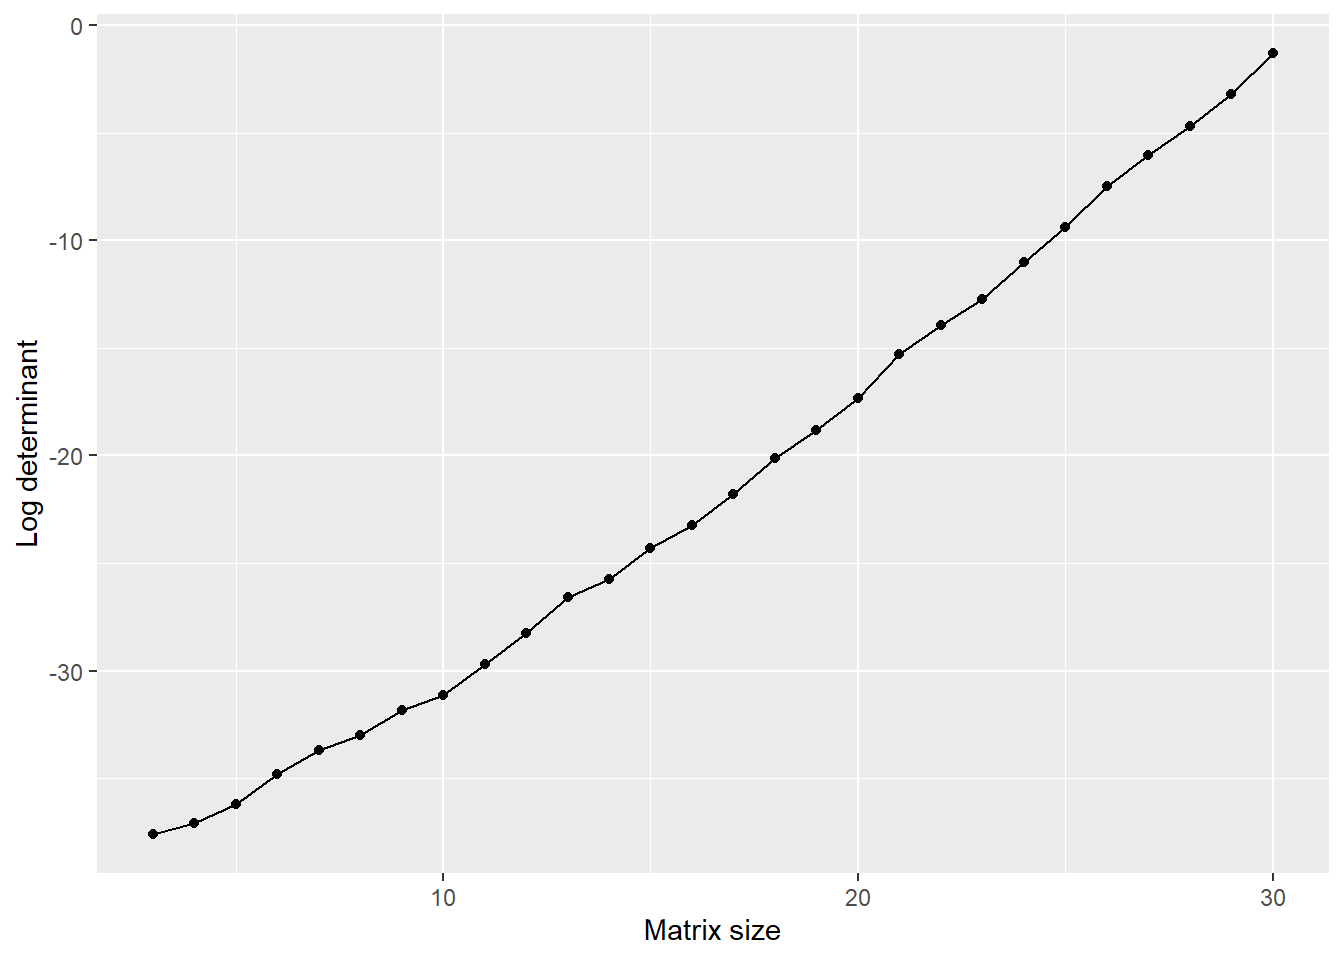
\includegraphics{cohen-linear-algebra_files/figure-latex/e11-2-1.pdf}

\hypertarget{chapter-12-1}{%
\section*{Chapter 12}\label{chapter-12-1}}
\addcontentsline{toc}{section}{Chapter 12}

\hypertarget{exercise-1-8}{%
\subsection*{Exercise 1}\label{exercise-1-8}}
\addcontentsline{toc}{subsection}{Exercise 1}

\begin{Shaded}
\begin{Highlighting}[]
\CommentTok{\# create matrix}
\NormalTok{m \textless{}{-}}\StringTok{ }\DecValTok{4}
\NormalTok{A \textless{}{-}}\StringTok{ }\KeywordTok{matrix}\NormalTok{(}\KeywordTok{rnorm}\NormalTok{(m}\OperatorTok{\^{}}\DecValTok{2}\NormalTok{), }\DataTypeTok{nrow=}\NormalTok{m, }\DataTypeTok{ncol=}\NormalTok{m)}
\NormalTok{M \textless{}{-}}\StringTok{ }\KeywordTok{matrix}\NormalTok{(}\DecValTok{0}\NormalTok{, }\DataTypeTok{nrow=}\NormalTok{m, }\DataTypeTok{ncol=}\NormalTok{m)}
\NormalTok{G \textless{}{-}}\StringTok{ }\KeywordTok{matrix}\NormalTok{(}\DecValTok{0}\NormalTok{, }\DataTypeTok{nrow=}\NormalTok{m, }\DataTypeTok{ncol=}\NormalTok{m)}

\CommentTok{\# compute minors matrix}
\ControlFlowTok{for}\NormalTok{(i }\ControlFlowTok{in} \DecValTok{1}\OperatorTok{:}\NormalTok{m)\{}
  \ControlFlowTok{for}\NormalTok{(j }\ControlFlowTok{in} \DecValTok{1}\OperatorTok{:}\NormalTok{m)\{}
    
    \CommentTok{\#\# select rows and cols}
    \CommentTok{\# implementation matching the original}
\NormalTok{    rows \textless{}{-}}\StringTok{ }\KeywordTok{rep}\NormalTok{(}\OtherTok{TRUE}\NormalTok{, m)}
\NormalTok{    rows[i] \textless{}{-}}\StringTok{ }\OtherTok{FALSE}
\NormalTok{    cols \textless{}{-}}\StringTok{ }\KeywordTok{rep}\NormalTok{(}\OtherTok{TRUE}\NormalTok{, m)}
\NormalTok{    cols[j] \textless{}{-}}\StringTok{ }\OtherTok{FALSE}
\NormalTok{    M[i, j] \textless{}{-}}\StringTok{ }\KeywordTok{det}\NormalTok{(A[rows, cols])}
    
    \CommentTok{\# a simpler R{-}version using negative (excluding) indexing}
\NormalTok{    M[i, j] \textless{}{-}}\StringTok{ }\KeywordTok{det}\NormalTok{(A[}\OperatorTok{{-}}\NormalTok{i, }\OperatorTok{{-}}\NormalTok{j])}
    
    \CommentTok{\# compute G}
\NormalTok{    G[i, j] \textless{}{-}}\StringTok{ }\NormalTok{(}\OperatorTok{{-}}\DecValTok{1}\NormalTok{)}\OperatorTok{\^{}}\NormalTok{(i }\OperatorTok{+}\StringTok{ }\NormalTok{j)}
\NormalTok{  \}}
\NormalTok{\}}

\CommentTok{\# compute C}
\NormalTok{C \textless{}{-}}\StringTok{ }\NormalTok{M }\OperatorTok{*}\StringTok{ }\NormalTok{G}

\CommentTok{\# compute A}
\NormalTok{Ainv \textless{}{-}}\StringTok{ }\KeywordTok{t}\NormalTok{(C) }\OperatorTok{/}\StringTok{ }\KeywordTok{det}\NormalTok{(A)}
\NormalTok{AinvI \textless{}{-}}\StringTok{ }\KeywordTok{solve}\NormalTok{(A)}
\KeywordTok{round}\NormalTok{(AinvI }\OperatorTok{{-}}\StringTok{ }\NormalTok{Ainv, }\DecValTok{4}\NormalTok{)}
\end{Highlighting}
\end{Shaded}

\begin{verbatim}
##      [,1] [,2] [,3] [,4]
## [1,]    0    0    0    0
## [2,]    0    0    0    0
## [3,]    0    0    0    0
## [4,]    0    0    0    0
\end{verbatim}

\hypertarget{exercise-2-8}{%
\subsection*{Exercise 2}\label{exercise-2-8}}
\addcontentsline{toc}{subsection}{Exercise 2}

I renamed \texttt{T} into \texttt{TM}, as \texttt{T} is a logical \texttt{TRUE} in R.

\begin{Shaded}
\begin{Highlighting}[]
\CommentTok{\# square matrix}
\NormalTok{A \textless{}{-}}\StringTok{ }\KeywordTok{matrix}\NormalTok{(}\KeywordTok{rnorm}\NormalTok{(}\DecValTok{5}\OperatorTok{\^{}}\DecValTok{2}\NormalTok{), }\DataTypeTok{nrow=}\DecValTok{5}\NormalTok{, }\DataTypeTok{ncol=}\DecValTok{5}\NormalTok{)}
\NormalTok{Ai \textless{}{-}}\StringTok{ }\KeywordTok{solve}\NormalTok{(A)}
\NormalTok{Api \textless{}{-}}\StringTok{ }\NormalTok{pracma}\OperatorTok{::}\KeywordTok{pinv}\NormalTok{(A)}
\KeywordTok{print}\NormalTok{(}\KeywordTok{round}\NormalTok{(Ai }\OperatorTok{{-}}\StringTok{ }\NormalTok{Api))}
\end{Highlighting}
\end{Shaded}

\begin{verbatim}
##      [,1] [,2] [,3] [,4] [,5]
## [1,]    0    0    0    0    0
## [2,]    0    0    0    0    0
## [3,]    0    0    0    0    0
## [4,]    0    0    0    0    0
## [5,]    0    0    0    0    0
\end{verbatim}

\begin{Shaded}
\begin{Highlighting}[]
\CommentTok{\# tall matrix}
\NormalTok{TM \textless{}{-}}\StringTok{ }\KeywordTok{matrix}\NormalTok{(}\KeywordTok{rnorm}\NormalTok{(}\DecValTok{5}\OperatorTok{*}\DecValTok{3}\NormalTok{), }\DataTypeTok{nrow=}\DecValTok{5}\NormalTok{, }\DataTypeTok{ncol=}\DecValTok{3}\NormalTok{)}
\NormalTok{TMl \textless{}{-}}\StringTok{ }\KeywordTok{solve}\NormalTok{(}\KeywordTok{t}\NormalTok{(TM) }\OperatorTok{\%*\%}\StringTok{ }\NormalTok{TM) }\OperatorTok{\%*\%}\StringTok{ }\KeywordTok{t}\NormalTok{(TM)}
\NormalTok{TMpi \textless{}{-}}\StringTok{ }\NormalTok{pracma}\OperatorTok{::}\KeywordTok{pinv}\NormalTok{(TM)}
\KeywordTok{print}\NormalTok{(}\KeywordTok{round}\NormalTok{(TMl }\OperatorTok{{-}}\StringTok{ }\NormalTok{TMpi))}
\end{Highlighting}
\end{Shaded}

\begin{verbatim}
##      [,1] [,2] [,3] [,4] [,5]
## [1,]    0    0    0    0    0
## [2,]    0    0    0    0    0
## [3,]    0    0    0    0    0
\end{verbatim}

\hypertarget{chapter-13-1}{%
\section*{Chapter 13}\label{chapter-13-1}}
\addcontentsline{toc}{section}{Chapter 13}

\hypertarget{exercise-2-9}{%
\subsection*{Exercise 2}\label{exercise-2-9}}
\addcontentsline{toc}{subsection}{Exercise 2}

\begin{Shaded}
\begin{Highlighting}[]
\NormalTok{m \textless{}{-}}\StringTok{ }\DecValTok{4}
\NormalTok{n \textless{}{-}}\StringTok{ }\DecValTok{4}
\NormalTok{A \textless{}{-}}\StringTok{ }\KeywordTok{matrix}\NormalTok{(}\KeywordTok{rnorm}\NormalTok{(}\DataTypeTok{n=}\NormalTok{m}\OperatorTok{*}\NormalTok{n), }\DataTypeTok{nrow=}\NormalTok{m, }\DataTypeTok{ncol=}\NormalTok{n)}
\NormalTok{Q \textless{}{-}}\StringTok{ }\KeywordTok{matrix}\NormalTok{(}\DecValTok{0}\NormalTok{, }\DataTypeTok{nrow=}\NormalTok{m, }\DataTypeTok{ncol=}\NormalTok{n)}

\ControlFlowTok{for}\NormalTok{(i }\ControlFlowTok{in} \DecValTok{1}\OperatorTok{:}\NormalTok{n)\{}
\NormalTok{  Q[, i] \textless{}{-}}\StringTok{ }\NormalTok{A[, i]}
  
  \CommentTok{\# orthogonalize}
\NormalTok{  a \textless{}{-}}\StringTok{ }\NormalTok{A[, i] }\CommentTok{\# convenience}
  \ControlFlowTok{if}\NormalTok{ (i }\OperatorTok{\textgreater{}}\StringTok{ }\DecValTok{1}\NormalTok{)\{}
    \ControlFlowTok{for}\NormalTok{(j }\ControlFlowTok{in} \DecValTok{1}\OperatorTok{:}\NormalTok{(i}\DecValTok{{-}1}\NormalTok{))\{}
\NormalTok{      q \textless{}{-}}\StringTok{ }\NormalTok{Q[, j] }\CommentTok{\# convenience}
\NormalTok{      Q[, i] \textless{}{-}}\StringTok{ }\NormalTok{Q[, i] }\OperatorTok{{-}}\StringTok{ }\NormalTok{pracma}\OperatorTok{::}\KeywordTok{dot}\NormalTok{(a, q) }\OperatorTok{/}\StringTok{ }\NormalTok{pracma}\OperatorTok{::}\KeywordTok{dot}\NormalTok{(q, q) }\OperatorTok{*}\StringTok{ }\NormalTok{q }
\NormalTok{    \}}
\NormalTok{  \}}
  
  \CommentTok{\# normalize}
\NormalTok{  Q[, i] \textless{}{-}}\StringTok{ }\NormalTok{Q[, i] }\OperatorTok{/}\StringTok{ }\KeywordTok{norm}\NormalTok{(}\KeywordTok{matrix}\NormalTok{(Q[, i]), }\DataTypeTok{type=}\StringTok{"F"}\NormalTok{)}
\NormalTok{\}}

\NormalTok{QR \textless{}{-}}\StringTok{ }\KeywordTok{qr}\NormalTok{(A)}
\NormalTok{Q2 \textless{}{-}}\StringTok{ }\KeywordTok{qr.Q}\NormalTok{(QR)}
\end{Highlighting}
\end{Shaded}

\hypertarget{chapter-14}{%
\section*{Chapter 14}\label{chapter-14}}
\addcontentsline{toc}{section}{Chapter 14}

\hypertarget{exercise-3-3}{%
\subsection*{Exercise 3}\label{exercise-3-3}}
\addcontentsline{toc}{subsection}{Exercise 3}

\begin{Shaded}
\begin{Highlighting}[]
\CommentTok{\# load the data into a table that we convert to a matrix}
\NormalTok{df \textless{}{-}}\StringTok{ }\KeywordTok{read.csv}\NormalTok{(}\StringTok{"http://sincxpress.com/widget\_data.txt"}\NormalTok{, }\DataTypeTok{header=}\OtherTok{FALSE}\NormalTok{)}
\NormalTok{data \textless{}{-}}\StringTok{ }\KeywordTok{as.matrix}\NormalTok{(df)}

\CommentTok{\# design matrix}
\NormalTok{X \textless{}{-}}\StringTok{ }\KeywordTok{cbind}\NormalTok{(}\KeywordTok{rep}\NormalTok{(}\DecValTok{1}\NormalTok{, }\KeywordTok{nrow}\NormalTok{(data)), data[, }\DecValTok{1}\OperatorTok{:}\DecValTok{2}\NormalTok{])}
\KeywordTok{colnames}\NormalTok{(X) \textless{}{-}}\StringTok{ }\KeywordTok{c}\NormalTok{(}\StringTok{"x1"}\NormalTok{, }\StringTok{"x2"}\NormalTok{, }\StringTok{"x3"}\NormalTok{)}

\CommentTok{\# outcome variable}
\NormalTok{y \textless{}{-}}\StringTok{ }\NormalTok{data[, }\DecValTok{3}\NormalTok{]}

\CommentTok{\# beta coefficients[]}
\NormalTok{beta \textless{}{-}}\StringTok{ }\KeywordTok{lsfit}\NormalTok{(X, y)}\OperatorTok{$}\NormalTok{coefficients[}\DecValTok{1}\OperatorTok{:}\DecValTok{3}\NormalTok{]}
\end{Highlighting}
\end{Shaded}

\begin{verbatim}
## Warning in lsfit(X, y): 'X' matrix was collinear
\end{verbatim}

\begin{Shaded}
\begin{Highlighting}[]
\CommentTok{\# scaled coefficients (intercept not scaled)}
\NormalTok{betaScaled \textless{}{-}}\StringTok{ }\NormalTok{beta }\OperatorTok{/}\StringTok{ }\KeywordTok{apply}\NormalTok{(X, }\DataTypeTok{MARGIN=}\DecValTok{2}\NormalTok{, }\DataTypeTok{FUN=}\NormalTok{sd)}
\end{Highlighting}
\end{Shaded}

\hypertarget{exercise-4-1}{%
\subsection*{Exercise 4}\label{exercise-4-1}}
\addcontentsline{toc}{subsection}{Exercise 4}

\begin{Shaded}
\begin{Highlighting}[]
\KeywordTok{library}\NormalTok{(dplyr)}
\KeywordTok{library}\NormalTok{(ggplot2)}
\KeywordTok{library}\NormalTok{(tidyr)}

\NormalTok{df\_long \textless{}{-}}
\StringTok{  }\NormalTok{df }\OperatorTok{\%\textgreater{}\%}
\StringTok{  }\NormalTok{dplyr}\OperatorTok{::}\KeywordTok{rename}\NormalTok{(}\StringTok{"Time of day"}\NormalTok{ =}\StringTok{ }\DecValTok{1}\NormalTok{, }\StringTok{"Age"}\NormalTok{ =}\StringTok{ }\DecValTok{2}\NormalTok{, }\StringTok{"Widgets purchased"}\NormalTok{=}\DecValTok{3}\NormalTok{) }\OperatorTok{\%\textgreater{}\%}
\StringTok{  }\NormalTok{tidyr}\OperatorTok{::}\KeywordTok{pivot\_longer}\NormalTok{(}\DataTypeTok{cols =} \KeywordTok{c}\NormalTok{(}\StringTok{"Time of day"}\NormalTok{, }\StringTok{"Age"}\NormalTok{), }\DataTypeTok{names\_to =} \StringTok{"Variable name"}\NormalTok{, }\DataTypeTok{values\_to =} \StringTok{"Variable"}\NormalTok{) }\OperatorTok{\%\textgreater{}\%}
\StringTok{  }\NormalTok{dplyr}\OperatorTok{::}\KeywordTok{mutate}\NormalTok{(}\StringTok{\textasciigrave{}}\DataTypeTok{Variable name}\StringTok{\textasciigrave{}}\NormalTok{ =}\StringTok{ }\KeywordTok{factor}\NormalTok{(}\StringTok{\textasciigrave{}}\DataTypeTok{Variable name}\StringTok{\textasciigrave{}}\NormalTok{, }\DataTypeTok{levels=}\KeywordTok{c}\NormalTok{(}\StringTok{"Time of day"}\NormalTok{, }\StringTok{"Age"}\NormalTok{)))}

\KeywordTok{ggplot}\NormalTok{(df\_long, }\KeywordTok{aes}\NormalTok{(}\DataTypeTok{x =}\NormalTok{ Variable, }\DataTypeTok{y=}\StringTok{\textasciigrave{}}\DataTypeTok{Widgets purchased}\StringTok{\textasciigrave{}}\NormalTok{)) }\OperatorTok{+}\StringTok{ }
\StringTok{  }\KeywordTok{geom\_point}\NormalTok{() }\OperatorTok{+}\StringTok{ }
\StringTok{  }\KeywordTok{facet\_grid}\NormalTok{(.}\OperatorTok{\textasciitilde{}}\StringTok{\textasciigrave{}}\DataTypeTok{Variable name}\StringTok{\textasciigrave{}}\NormalTok{, }\DataTypeTok{scales=}\StringTok{"free\_x"}\NormalTok{)}
\end{Highlighting}
\end{Shaded}

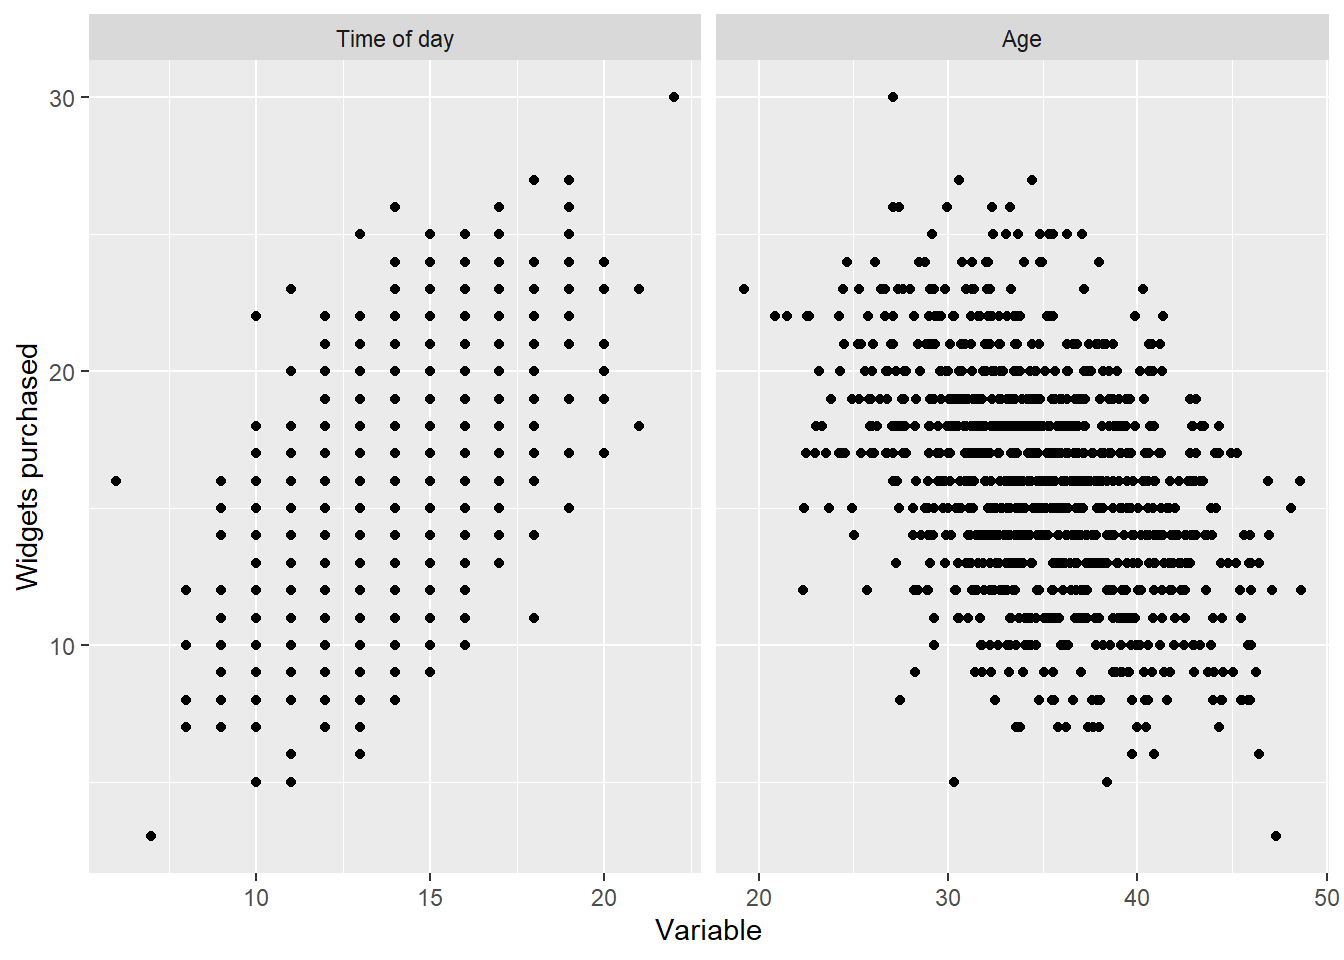
\includegraphics{cohen-linear-algebra_files/figure-latex/e14-4-1.pdf}

\hypertarget{exercise-5}{%
\subsection*{Exercise 5}\label{exercise-5}}
\addcontentsline{toc}{subsection}{Exercise 5}

\begin{Shaded}
\begin{Highlighting}[]
\NormalTok{yHat \textless{}{-}}\StringTok{ }\NormalTok{X }\OperatorTok{\%*\%}\StringTok{ }\NormalTok{beta}
\NormalTok{r2 \textless{}{-}}\StringTok{ }\DecValTok{1} \OperatorTok{{-}}\StringTok{ }\KeywordTok{sum}\NormalTok{((yHat }\OperatorTok{{-}}\StringTok{ }\NormalTok{y)}\OperatorTok{\^{}}\DecValTok{2}\NormalTok{) }\OperatorTok{/}\StringTok{ }\KeywordTok{sum}\NormalTok{((y }\OperatorTok{{-}}\StringTok{ }\KeywordTok{mean}\NormalTok{(y))}\OperatorTok{\^{}}\DecValTok{2}\NormalTok{)}
\end{Highlighting}
\end{Shaded}

\hypertarget{chapter-15-1}{%
\section*{Chapter 15}\label{chapter-15-1}}
\addcontentsline{toc}{section}{Chapter 15}

\hypertarget{exercise-1-9}{%
\subsection*{Exercise 1}\label{exercise-1-9}}
\addcontentsline{toc}{subsection}{Exercise 1}

\begin{Shaded}
\begin{Highlighting}[]
\NormalTok{avediffs \textless{}{-}}\StringTok{ }\KeywordTok{rep}\NormalTok{(}\DecValTok{0}\NormalTok{, }\DataTypeTok{times=}\DecValTok{100}\NormalTok{)}
\ControlFlowTok{for}\NormalTok{(n }\ControlFlowTok{in} \DecValTok{1}\OperatorTok{:}\DecValTok{100}\NormalTok{)\{}
\NormalTok{  A \textless{}{-}}\StringTok{ }\KeywordTok{matrix}\NormalTok{(}\KeywordTok{rnorm}\NormalTok{(}\DataTypeTok{n=}\NormalTok{n}\OperatorTok{\^{}}\DecValTok{2}\NormalTok{), }\DataTypeTok{nrow=}\NormalTok{n, }\DataTypeTok{ncol=}\NormalTok{n)}
\NormalTok{  B \textless{}{-}}\StringTok{ }\KeywordTok{matrix}\NormalTok{(}\KeywordTok{rnorm}\NormalTok{(}\DataTypeTok{n=}\NormalTok{n}\OperatorTok{\^{}}\DecValTok{2}\NormalTok{), }\DataTypeTok{nrow=}\NormalTok{n, }\DataTypeTok{ncol=}\NormalTok{n)}
\NormalTok{  l1 \textless{}{-}}\StringTok{ }\NormalTok{geigen}\OperatorTok{::}\KeywordTok{geigen}\NormalTok{(A, B, }\DataTypeTok{symmetric=}\OtherTok{FALSE}\NormalTok{, }\DataTypeTok{only.values=}\OtherTok{TRUE}\NormalTok{)}\OperatorTok{$}\NormalTok{values}
\NormalTok{  l2 \textless{}{-}}\StringTok{ }\KeywordTok{eigen}\NormalTok{(}\KeywordTok{solve}\NormalTok{(B) }\OperatorTok{\%*\%}\StringTok{ }\NormalTok{A)}\OperatorTok{$}\NormalTok{values}
  
  \CommentTok{\# important to sort eigvals}
\NormalTok{  l1 \textless{}{-}}\StringTok{ }\KeywordTok{sort}\NormalTok{(l1)}
\NormalTok{  l2 \textless{}{-}}\StringTok{ }\KeywordTok{sort}\NormalTok{(l2)}
  
\NormalTok{  avediffs[n] \textless{}{-}}\StringTok{ }\KeywordTok{mean}\NormalTok{(}\KeywordTok{abs}\NormalTok{(l1}\OperatorTok{{-}}\NormalTok{l2))}
\NormalTok{\}}

\KeywordTok{ggplot}\NormalTok{(}\DataTypeTok{data=}\OtherTok{NULL}\NormalTok{, }\KeywordTok{aes}\NormalTok{(}\DataTypeTok{x=}\DecValTok{1}\OperatorTok{:}\DecValTok{100}\NormalTok{, }\DataTypeTok{y=}\NormalTok{avediffs)) }\OperatorTok{+}\StringTok{ }
\StringTok{  }\KeywordTok{geom\_point}\NormalTok{() }\OperatorTok{+}\StringTok{ }
\StringTok{  }\KeywordTok{xlab}\NormalTok{(}\StringTok{"Matrix size"}\NormalTok{) }\OperatorTok{+}\StringTok{ }
\StringTok{  }\KeywordTok{ylab}\NormalTok{(}\KeywordTok{expression}\NormalTok{(}\KeywordTok{paste}\NormalTok{(Delta, lambda)))}
\end{Highlighting}
\end{Shaded}

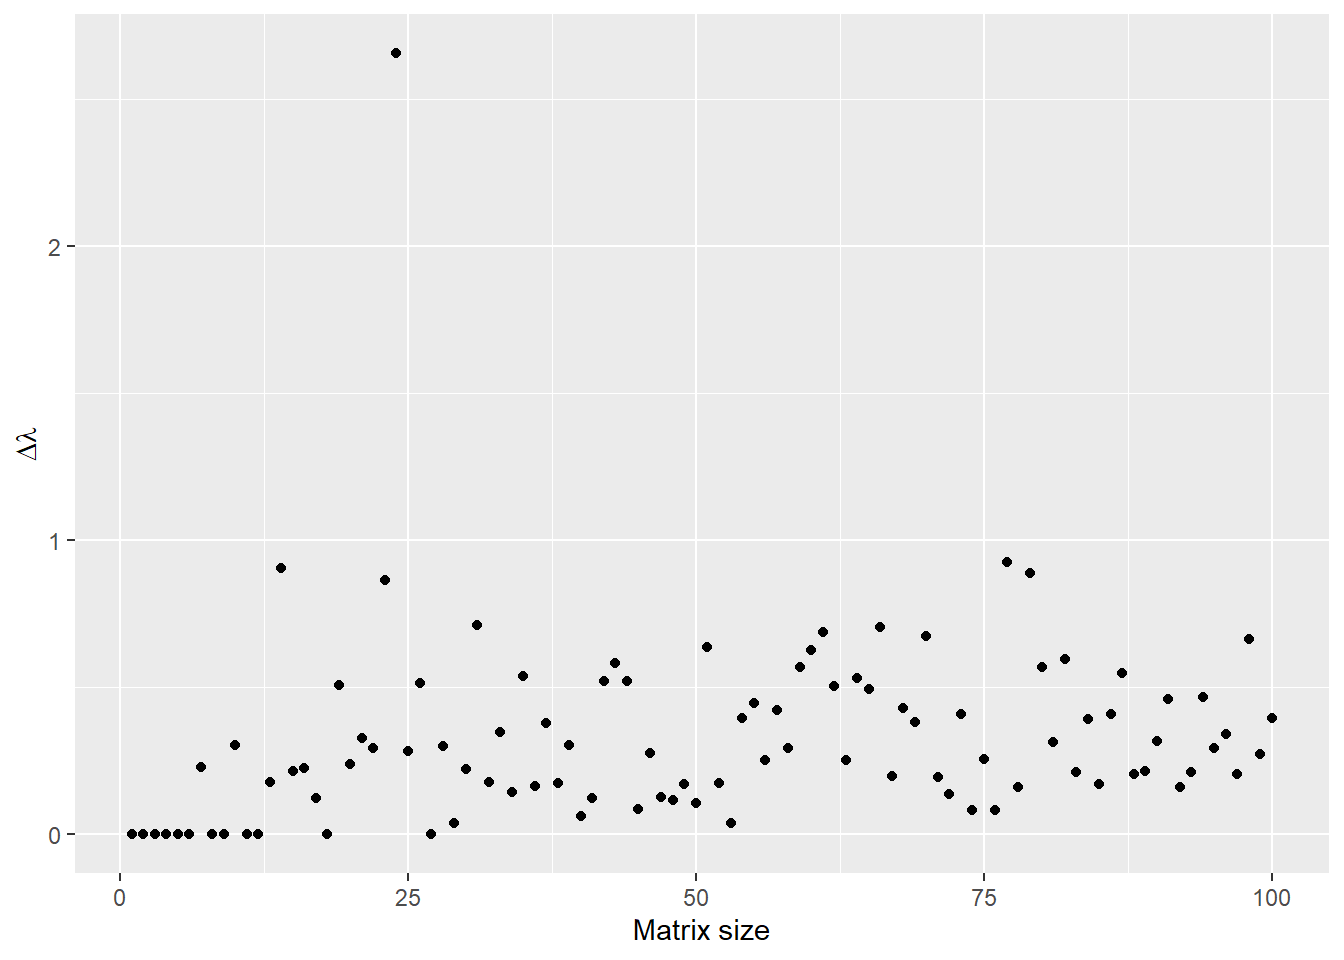
\includegraphics{cohen-linear-algebra_files/figure-latex/e15-1-1.pdf}

\hypertarget{exercise-2-10}{%
\subsection*{Exercise 2}\label{exercise-2-10}}
\addcontentsline{toc}{subsection}{Exercise 2}

\begin{Shaded}
\begin{Highlighting}[]
\NormalTok{A \textless{}{-}}\StringTok{ }\KeywordTok{diag}\NormalTok{(}\DecValTok{1}\OperatorTok{:}\DecValTok{6}\NormalTok{)}
\NormalTok{eigenA \textless{}{-}}\StringTok{ }\KeywordTok{eigen}\NormalTok{(A)}
\NormalTok{L \textless{}{-}}\StringTok{ }\NormalTok{eigenA}\OperatorTok{$}\NormalTok{values}
\NormalTok{V \textless{}{-}}\StringTok{ }\NormalTok{eigenA}\OperatorTok{$}\NormalTok{vectors}
\end{Highlighting}
\end{Shaded}

\hypertarget{exercise-3-4}{%
\subsection*{Exercise 3}\label{exercise-3-4}}
\addcontentsline{toc}{subsection}{Exercise 3}

\begin{Shaded}
\begin{Highlighting}[]
\KeywordTok{library}\NormalTok{(dplyr)}
\KeywordTok{library}\NormalTok{(ggplot2)}
\KeywordTok{library}\NormalTok{(patchwork)}
\KeywordTok{library}\NormalTok{(reshape2)}

\NormalTok{v \textless{}{-}}\StringTok{ }\DecValTok{1}\OperatorTok{:}\DecValTok{50}
\NormalTok{lstrow \textless{}{-}}\StringTok{ }\KeywordTok{c}\NormalTok{(v[}\KeywordTok{length}\NormalTok{(v)], v[}\OperatorTok{{-}}\KeywordTok{length}\NormalTok{(v)])}
\NormalTok{H \textless{}{-}}\StringTok{ }\NormalTok{pracma}\OperatorTok{::}\KeywordTok{hankel}\NormalTok{(v, lstrow)}
\NormalTok{eigH \textless{}{-}}\StringTok{ }\KeywordTok{eigen}\NormalTok{(H)}
\NormalTok{V \textless{}{-}}\StringTok{ }\NormalTok{eigH}\OperatorTok{$}\NormalTok{vectors[, }\KeywordTok{order}\NormalTok{(eigH}\OperatorTok{$}\NormalTok{values, }\DataTypeTok{decreasing=}\OtherTok{TRUE}\NormalTok{)]}

\CommentTok{\# the matrix}
\NormalTok{plotH \textless{}{-}}\StringTok{ }
\StringTok{  }\KeywordTok{ggplot}\NormalTok{(}\DataTypeTok{data=}\NormalTok{reshape2}\OperatorTok{::}\KeywordTok{melt}\NormalTok{(H), }\KeywordTok{aes}\NormalTok{(}\DataTypeTok{x=}\DecValTok{1}\OperatorTok{{-}}\NormalTok{Var1, }\DataTypeTok{y=}\NormalTok{Var2)) }\OperatorTok{+}\StringTok{ }
\StringTok{  }\KeywordTok{geom\_raster}\NormalTok{(}\KeywordTok{aes}\NormalTok{(}\DataTypeTok{fill=}\NormalTok{value), }\DataTypeTok{show.legend=}\OtherTok{FALSE}\NormalTok{) }\OperatorTok{+}\StringTok{ }
\StringTok{  }\KeywordTok{labs}\NormalTok{(}\DataTypeTok{title=}\StringTok{"Hankel matrix"}\NormalTok{) }\OperatorTok{+}\StringTok{ }
\StringTok{  }\KeywordTok{coord\_equal}\NormalTok{() }\OperatorTok{+}\StringTok{ }\KeywordTok{xlab}\NormalTok{(}\StringTok{""}\NormalTok{) }\OperatorTok{+}\StringTok{ }\KeywordTok{ylab}\NormalTok{(}\StringTok{""}\NormalTok{)}
  

\CommentTok{\# eigenvector matrix}
\NormalTok{plotV \textless{}{-}}\StringTok{ }
\StringTok{  }\KeywordTok{ggplot}\NormalTok{(}\DataTypeTok{data=}\NormalTok{reshape2}\OperatorTok{::}\KeywordTok{melt}\NormalTok{(V), }\KeywordTok{aes}\NormalTok{(}\DataTypeTok{x=}\NormalTok{Var2, }\DataTypeTok{y=}\NormalTok{Var1)) }\OperatorTok{+}\StringTok{ }
\StringTok{  }\KeywordTok{geom\_raster}\NormalTok{(}\KeywordTok{aes}\NormalTok{(}\DataTypeTok{fill=}\NormalTok{value), }\DataTypeTok{show.legend=}\OtherTok{FALSE}\NormalTok{) }\OperatorTok{+}\StringTok{ }
\StringTok{  }\KeywordTok{labs}\NormalTok{(}\DataTypeTok{title=}\StringTok{"Eigenvector matrix"}\NormalTok{) }\OperatorTok{+}\StringTok{ }
\StringTok{  }\KeywordTok{coord\_equal}\NormalTok{() }\OperatorTok{+}\StringTok{ }\KeywordTok{xlab}\NormalTok{(}\StringTok{""}\NormalTok{) }\OperatorTok{+}\StringTok{ }\KeywordTok{ylab}\NormalTok{(}\StringTok{""}\NormalTok{)}

\CommentTok{\# a few eigenvectors}
\NormalTok{dfV \textless{}{-}}\StringTok{ }
\StringTok{  }\KeywordTok{data.frame}\NormalTok{(}\KeywordTok{t}\NormalTok{(V)) }\OperatorTok{\%\textgreater{}\%}
\StringTok{  }\NormalTok{dplyr}\OperatorTok{::}\KeywordTok{slice\_head}\NormalTok{(}\DataTypeTok{n=}\DecValTok{4}\NormalTok{) }\OperatorTok{\%\textgreater{}\%}
\StringTok{  }\NormalTok{dplyr}\OperatorTok{::}\KeywordTok{mutate}\NormalTok{(}\DataTypeTok{VectorIndex =} \DecValTok{1}\OperatorTok{:}\KeywordTok{n}\NormalTok{()) }\OperatorTok{\%\textgreater{}\%}
\StringTok{  }\NormalTok{tidyr}\OperatorTok{::}\KeywordTok{pivot\_longer}\NormalTok{(}\DataTypeTok{cols =} \KeywordTok{c}\NormalTok{(X1}\OperatorTok{:}\NormalTok{X50), }\DataTypeTok{names\_to=}\StringTok{"Element"}\NormalTok{, }\DataTypeTok{values\_to=}\StringTok{"Value"}\NormalTok{) }\OperatorTok{\%\textgreater{}\%}
\StringTok{  }\NormalTok{dplyr}\OperatorTok{::}\KeywordTok{group\_by}\NormalTok{(VectorIndex) }\OperatorTok{\%\textgreater{}\%}
\StringTok{  }\NormalTok{dplyr}\OperatorTok{::}\KeywordTok{mutate}\NormalTok{(}\DataTypeTok{ElementIndex =} \DecValTok{1}\OperatorTok{:}\KeywordTok{n}\NormalTok{()) }\OperatorTok{\%\textgreater{}\%}
\StringTok{  }\NormalTok{dplyr}\OperatorTok{::}\KeywordTok{select}\NormalTok{(}\OperatorTok{{-}}\NormalTok{Element)}

\NormalTok{plot4 \textless{}{-}}\StringTok{ }
\StringTok{  }\KeywordTok{ggplot}\NormalTok{(}\DataTypeTok{data=}\NormalTok{dfV, }\KeywordTok{aes}\NormalTok{(}\DataTypeTok{x =}\NormalTok{ ElementIndex, }\DataTypeTok{y=}\NormalTok{Value, }\DataTypeTok{color=}\KeywordTok{as.factor}\NormalTok{(VectorIndex))) }\OperatorTok{+}\StringTok{ }
\StringTok{  }\KeywordTok{geom\_line}\NormalTok{(}\DataTypeTok{show.legend=}\OtherTok{FALSE}\NormalTok{) }\OperatorTok{+}\StringTok{ }
\StringTok{  }\KeywordTok{geom\_point}\NormalTok{(}\DataTypeTok{show.legend=}\OtherTok{FALSE}\NormalTok{) }\OperatorTok{+}\StringTok{ }
\StringTok{  }\KeywordTok{xlab}\NormalTok{(}\StringTok{"Eigenvector element index"}\NormalTok{) }\OperatorTok{+}\StringTok{ }
\StringTok{  }\KeywordTok{ylab}\NormalTok{(}\StringTok{"Eigenvector element value"}\NormalTok{) }\OperatorTok{+}\StringTok{ }
\StringTok{  }\KeywordTok{labs}\NormalTok{(}\DataTypeTok{title =} \StringTok{"First four eigenvectors"}\NormalTok{)}

\NormalTok{(plotH }\OperatorTok{|}\StringTok{ }\NormalTok{plotV) }\OperatorTok{/}\StringTok{ }\NormalTok{plot4}
\end{Highlighting}
\end{Shaded}

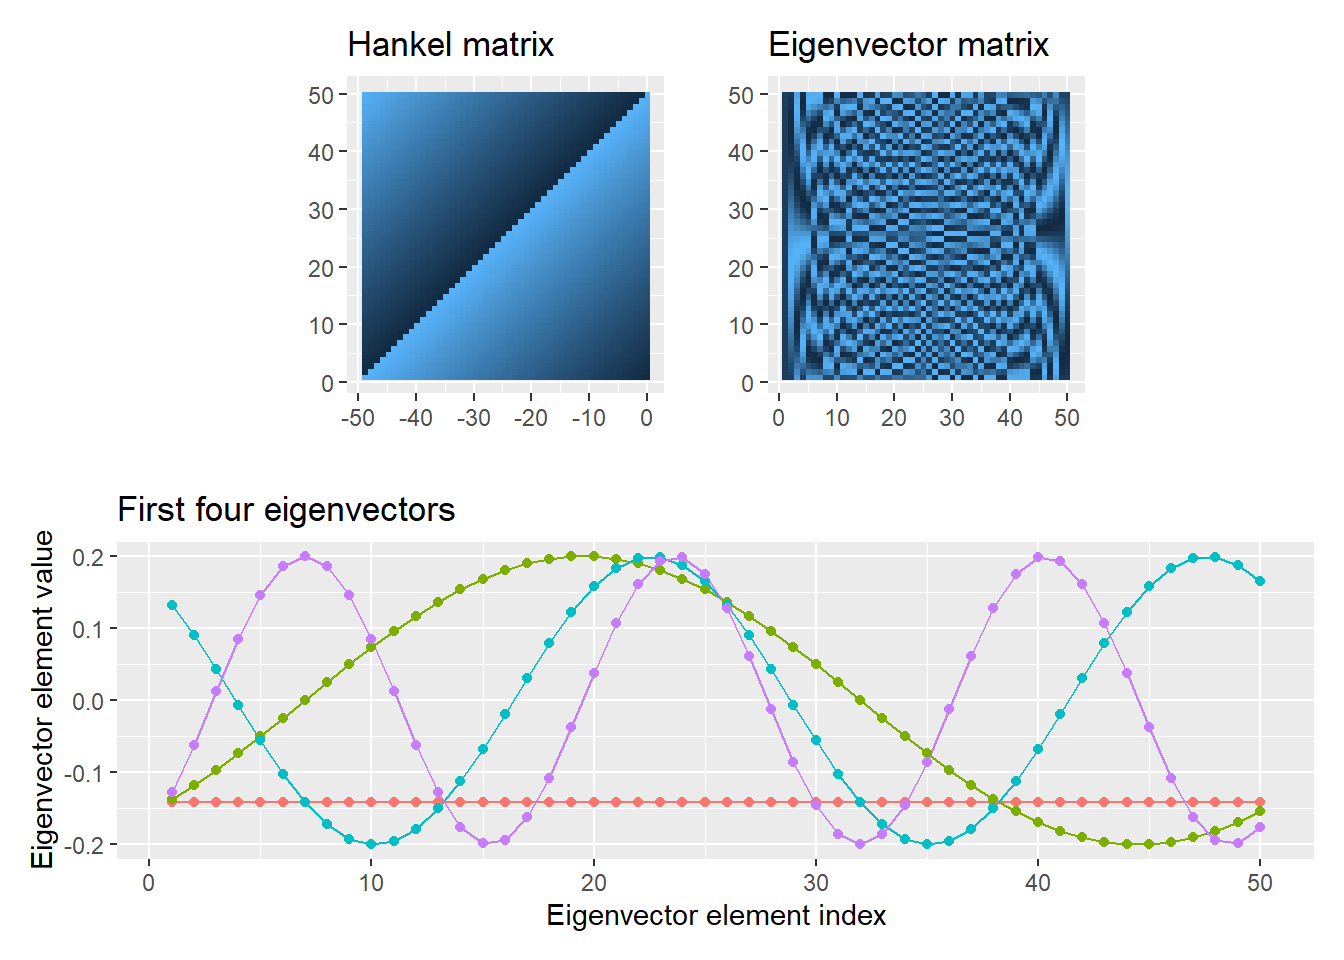
\includegraphics{cohen-linear-algebra_files/figure-latex/e15-3-1.pdf}

\hypertarget{chapter-16-1}{%
\section*{Chapter 16}\label{chapter-16-1}}
\addcontentsline{toc}{section}{Chapter 16}

\hypertarget{exercise-1-10}{%
\subsection*{Exercise 1}\label{exercise-1-10}}
\addcontentsline{toc}{subsection}{Exercise 1}

In R \href{https://stat.ethz.ch/R-manual/R-patched/library/base/html/svd.html}{svd()} defaults to ``economy'' mode. If you want the full matrix, you must specify dimensions for \textbf{U} and \textbf{V} explicitly.

\begin{Shaded}
\begin{Highlighting}[]
\NormalTok{m \textless{}{-}}\StringTok{ }\DecValTok{6}
\NormalTok{n \textless{}{-}}\StringTok{ }\DecValTok{3}
\NormalTok{A \textless{}{-}}\StringTok{ }\KeywordTok{matrix}\NormalTok{(}\KeywordTok{rnorm}\NormalTok{(}\DataTypeTok{n=}\NormalTok{m}\OperatorTok{*}\NormalTok{n), }\DataTypeTok{nrow=}\NormalTok{m, }\DataTypeTok{ncol=}\NormalTok{n)}

\NormalTok{fullSVD \textless{}{-}}\StringTok{ }\KeywordTok{svd}\NormalTok{(A, }\DataTypeTok{nu=}\NormalTok{m, }\DataTypeTok{nv=}\NormalTok{n)}
\NormalTok{economySVD \textless{}{-}}\StringTok{ }\KeywordTok{svd}\NormalTok{(A)}

\KeywordTok{cat}\NormalTok{(}\KeywordTok{sprintf}\NormalTok{(}\StringTok{"Full SVD: (\%d, \%d), \%d, (\%d, \%d)}\CharTok{\textbackslash{}n}\StringTok{"}\NormalTok{, }\KeywordTok{nrow}\NormalTok{(fullSVD}\OperatorTok{$}\NormalTok{u), }\KeywordTok{ncol}\NormalTok{(fullSVD}\OperatorTok{$}\NormalTok{u), }\KeywordTok{length}\NormalTok{(fullSVD}\OperatorTok{$}\NormalTok{d), }\KeywordTok{nrow}\NormalTok{(fullSVD}\OperatorTok{$}\NormalTok{v), }\KeywordTok{ncol}\NormalTok{(fullSVD}\OperatorTok{$}\NormalTok{v)))}
\end{Highlighting}
\end{Shaded}

\begin{verbatim}
## Full SVD: (6, 6), 3, (3, 3)
\end{verbatim}

\begin{Shaded}
\begin{Highlighting}[]
\KeywordTok{cat}\NormalTok{(}\KeywordTok{sprintf}\NormalTok{(}\StringTok{"Economy : (\%d, \%d), \%d, (\%d, \%d)}\CharTok{\textbackslash{}n}\StringTok{"}\NormalTok{, }\KeywordTok{nrow}\NormalTok{(economySVD}\OperatorTok{$}\NormalTok{u), }\KeywordTok{ncol}\NormalTok{(economySVD}\OperatorTok{$}\NormalTok{u), }\KeywordTok{length}\NormalTok{(economySVD}\OperatorTok{$}\NormalTok{d), }\KeywordTok{nrow}\NormalTok{(economySVD}\OperatorTok{$}\NormalTok{v), }\KeywordTok{ncol}\NormalTok{(economySVD}\OperatorTok{$}\NormalTok{v)))}
\end{Highlighting}
\end{Shaded}

\begin{verbatim}
## Economy : (6, 3), 3, (3, 3)
\end{verbatim}

\hypertarget{exercise-2-11}{%
\subsection*{Exercise 2}\label{exercise-2-11}}
\addcontentsline{toc}{subsection}{Exercise 2}

Note that \href{}{eigen()} sorts eigenvalues and eigenvectors, so sorting is redundant and can be skipped (but I kept it to match the original code).

\begin{Shaded}
\begin{Highlighting}[]
\NormalTok{A \textless{}{-}}\StringTok{ }\KeywordTok{matrix}\NormalTok{(}\KeywordTok{rnorm}\NormalTok{(}\DataTypeTok{n=}\DecValTok{4}\OperatorTok{*}\DecValTok{5}\NormalTok{), }\DataTypeTok{nrow=}\DecValTok{4}\NormalTok{, }\DataTypeTok{ncol=}\DecValTok{5}\NormalTok{) }\CommentTok{\# matrix}
\NormalTok{A \textless{}{-}}\StringTok{ }\KeywordTok{matrix}\NormalTok{(a, }\DataTypeTok{nrow=}\DecValTok{4}\NormalTok{, }\DataTypeTok{ncol=}\DecValTok{5}\NormalTok{, }\DataTypeTok{byrow=}\OtherTok{TRUE}\NormalTok{)}
\NormalTok{eigAV \textless{}{-}}\StringTok{ }\KeywordTok{eigen}\NormalTok{(}\KeywordTok{t}\NormalTok{(A) }\OperatorTok{\%*\%}\StringTok{ }\NormalTok{A) }
\NormalTok{V \textless{}{-}}\StringTok{  }\NormalTok{eigAV}\OperatorTok{$}\NormalTok{vectors[, }\KeywordTok{order}\NormalTok{(eigAV}\OperatorTok{$}\NormalTok{values, }\DataTypeTok{decreasing=}\OtherTok{TRUE}\NormalTok{)] }\CommentTok{\# sort descent V}
\NormalTok{eigAU \textless{}{-}}\StringTok{ }\KeywordTok{eigen}\NormalTok{(A }\OperatorTok{\%*\%}\StringTok{ }\KeywordTok{t}\NormalTok{(A)) }
\NormalTok{U \textless{}{-}}\StringTok{  }\NormalTok{eigAU}\OperatorTok{$}\NormalTok{vectors[, }\KeywordTok{order}\NormalTok{(eigAU}\OperatorTok{$}\NormalTok{values, }\DataTypeTok{decreasing=}\OtherTok{TRUE}\NormalTok{)] }\CommentTok{\# sort descent U}

\CommentTok{\# create Sigma}
\NormalTok{sorted\_values \textless{}{-}}\StringTok{ }\KeywordTok{sort}\NormalTok{(eigAU}\OperatorTok{$}\NormalTok{values, }\DataTypeTok{decreasing=}\OtherTok{TRUE}\NormalTok{)}
\NormalTok{S \textless{}{-}}\StringTok{ }\KeywordTok{matrix}\NormalTok{(}\DecValTok{0}\NormalTok{, }\DataTypeTok{nrow=}\KeywordTok{nrow}\NormalTok{(A), }\DataTypeTok{ncol=}\KeywordTok{ncol}\NormalTok{(A))}
\ControlFlowTok{for}\NormalTok{(i }\ControlFlowTok{in} \DecValTok{1}\OperatorTok{:}\KeywordTok{length}\NormalTok{(sorted\_values))\{}
\NormalTok{  S[i, i] \textless{}{-}}\StringTok{ }\KeywordTok{sqrt}\NormalTok{(sorted\_values[i])}
\NormalTok{\}}

\NormalTok{svdA \textless{}{-}}\StringTok{ }\KeywordTok{svd}\NormalTok{(A) }\CommentTok{\# svd}
\end{Highlighting}
\end{Shaded}

\hypertarget{exercise-3-5}{%
\subsection*{Exercise 3}\label{exercise-3-5}}
\addcontentsline{toc}{subsection}{Exercise 3}

\begin{Shaded}
\begin{Highlighting}[]
\KeywordTok{library}\NormalTok{(ggplot2)}
\KeywordTok{library}\NormalTok{(patchwork)}
\KeywordTok{library}\NormalTok{(RColorBrewer)}
\KeywordTok{library}\NormalTok{(reshape2)}


\NormalTok{A \textless{}{-}}\StringTok{ }\KeywordTok{matrix}\NormalTok{(}\KeywordTok{rnorm}\NormalTok{(}\DataTypeTok{n=}\DecValTok{5}\OperatorTok{*}\DecValTok{3}\NormalTok{), }\DataTypeTok{nrow=}\DecValTok{5}\NormalTok{, }\DataTypeTok{ncol=}\DecValTok{3}\NormalTok{)}
\NormalTok{svdA \textless{}{-}}\StringTok{ }\KeywordTok{svd}\NormalTok{(A)}
\NormalTok{S \textless{}{-}}\StringTok{ }\KeywordTok{diag}\NormalTok{(svdA}\OperatorTok{$}\NormalTok{d) }\CommentTok{\# need Sigma matrix}

\NormalTok{fill\_palette \textless{}{-}}\StringTok{ }\KeywordTok{colorRampPalette}\NormalTok{(}\KeywordTok{rev}\NormalTok{(}\KeywordTok{brewer.pal}\NormalTok{(}\DecValTok{11}\NormalTok{, }\StringTok{"Spectral"}\NormalTok{)))}
\NormalTok{sc \textless{}{-}}\StringTok{ }\KeywordTok{scale\_colour\_gradientn}\NormalTok{(}\DataTypeTok{colours =} \KeywordTok{fill\_palette}\NormalTok{(}\DecValTok{100}\NormalTok{), }\DataTypeTok{limits=}\KeywordTok{c}\NormalTok{(}\KeywordTok{min}\NormalTok{(A), }\KeywordTok{max}\NormalTok{(A)))}


\NormalTok{one\_layer\_plots \textless{}{-}}\StringTok{ }\KeywordTok{list}\NormalTok{()}
\NormalTok{lowrank\_plots \textless{}{-}}\StringTok{ }\KeywordTok{list}\NormalTok{()}
\ControlFlowTok{for}\NormalTok{(i }\ControlFlowTok{in} \DecValTok{1}\OperatorTok{:}\DecValTok{3}\NormalTok{) \{}
\NormalTok{  onelayer \textless{}{-}}\StringTok{ }\KeywordTok{outer}\NormalTok{(svdA}\OperatorTok{$}\NormalTok{u[, i], svdA}\OperatorTok{$}\NormalTok{v[i, ]) }\OperatorTok{*}\StringTok{ }\NormalTok{svdA}\OperatorTok{$}\NormalTok{d[i]}
\NormalTok{  one\_layer\_plots[[i]] \textless{}{-}}\StringTok{ }
\StringTok{    }\KeywordTok{ggplot}\NormalTok{(}\DataTypeTok{data=}\NormalTok{reshape2}\OperatorTok{::}\KeywordTok{melt}\NormalTok{(}\KeywordTok{t}\NormalTok{(onelayer)), }\KeywordTok{aes}\NormalTok{(}\DataTypeTok{x=}\NormalTok{Var1, }\DataTypeTok{y=}\NormalTok{Var2, }\DataTypeTok{fill=}\NormalTok{value)) }\OperatorTok{+}\StringTok{ }
\StringTok{    }\KeywordTok{geom\_tile}\NormalTok{(}\DataTypeTok{show.legend=}\OtherTok{FALSE}\NormalTok{) }\OperatorTok{+}\StringTok{ }\KeywordTok{theme\_void}\NormalTok{() }\OperatorTok{+}
\StringTok{    }\KeywordTok{labs}\NormalTok{(}\DataTypeTok{title=}\KeywordTok{sprintf}\NormalTok{(}\StringTok{"Layer \%d"}\NormalTok{, i)) }\OperatorTok{+}
\StringTok{    }\KeywordTok{coord\_equal}\NormalTok{() }\OperatorTok{+}\StringTok{ }\NormalTok{sc}
  
\NormalTok{  lowrank \textless{}{-}}\StringTok{ }\KeywordTok{matrix}\NormalTok{(svdA}\OperatorTok{$}\NormalTok{u[, }\DecValTok{1}\OperatorTok{:}\NormalTok{i], }\DataTypeTok{ncol=}\NormalTok{i) }\OperatorTok{\%*\%}\StringTok{ }\NormalTok{S[}\DecValTok{1}\OperatorTok{:}\NormalTok{i,}\DecValTok{1}\OperatorTok{:}\NormalTok{i] }\OperatorTok{\%*\%}\StringTok{ }\KeywordTok{t}\NormalTok{(svdA}\OperatorTok{$}\NormalTok{v)[}\DecValTok{1}\OperatorTok{:}\NormalTok{i,]}
\NormalTok{  lowrank\_plots[[i]] \textless{}{-}}\StringTok{ }
\StringTok{    }\KeywordTok{ggplot}\NormalTok{(}\DataTypeTok{data=}\NormalTok{reshape2}\OperatorTok{::}\KeywordTok{melt}\NormalTok{(}\KeywordTok{t}\NormalTok{(lowrank)), }\KeywordTok{aes}\NormalTok{(}\DataTypeTok{x=}\NormalTok{Var1, }\DataTypeTok{y=}\NormalTok{Var2, }\DataTypeTok{fill=}\NormalTok{value)) }\OperatorTok{+}\StringTok{ }
\StringTok{    }\KeywordTok{geom\_tile}\NormalTok{(}\DataTypeTok{show.legend=}\OtherTok{FALSE}\NormalTok{) }\OperatorTok{+}\StringTok{ }\KeywordTok{theme\_void}\NormalTok{() }\OperatorTok{+}
\StringTok{    }\KeywordTok{labs}\NormalTok{(}\DataTypeTok{title=}\KeywordTok{sprintf}\NormalTok{(}\StringTok{"Layers 1:\%d"}\NormalTok{, i)) }\OperatorTok{+}
\StringTok{    }\KeywordTok{coord\_equal}\NormalTok{() }\OperatorTok{+}\StringTok{ }\NormalTok{sc}
\NormalTok{\}}

\NormalTok{plotA \textless{}{-}}\StringTok{ }
\StringTok{  }\KeywordTok{ggplot}\NormalTok{(}\DataTypeTok{data=}\NormalTok{reshape2}\OperatorTok{::}\KeywordTok{melt}\NormalTok{(}\KeywordTok{t}\NormalTok{(A)), }\KeywordTok{aes}\NormalTok{(}\DataTypeTok{x=}\NormalTok{Var1, }\DataTypeTok{y=}\NormalTok{Var2, }\DataTypeTok{fill=}\NormalTok{value)) }\OperatorTok{+}\StringTok{ }
\StringTok{  }\KeywordTok{geom\_tile}\NormalTok{(}\DataTypeTok{show.legend=}\OtherTok{FALSE}\NormalTok{) }\OperatorTok{+}\StringTok{ }\KeywordTok{theme\_void}\NormalTok{() }\OperatorTok{+}
\StringTok{  }\KeywordTok{labs}\NormalTok{(}\DataTypeTok{title=}\StringTok{"Orig. A"}\NormalTok{) }\OperatorTok{+}
\StringTok{  }\KeywordTok{coord\_equal}\NormalTok{() }\OperatorTok{+}\StringTok{ }\NormalTok{sc}

\NormalTok{layout \textless{}{-}}\StringTok{ "}
\StringTok{ABC\#}
\StringTok{DEFG}
\StringTok{"}
\NormalTok{one\_layer\_plots[[}\DecValTok{1}\NormalTok{]] }\OperatorTok{+}\StringTok{ }\NormalTok{one\_layer\_plots[[}\DecValTok{2}\NormalTok{]] }\OperatorTok{+}\StringTok{ }\NormalTok{one\_layer\_plots[[}\DecValTok{3}\NormalTok{]] }\OperatorTok{+}
\StringTok{  }\NormalTok{lowrank\_plots[[}\DecValTok{1}\NormalTok{]] }\OperatorTok{+}\StringTok{ }\NormalTok{lowrank\_plots[[}\DecValTok{2}\NormalTok{]] }\OperatorTok{+}\StringTok{ }\NormalTok{lowrank\_plots[[}\DecValTok{3}\NormalTok{]] }\OperatorTok{+}\StringTok{ }\NormalTok{plotA }\OperatorTok{+}
\StringTok{  }\KeywordTok{plot\_layout}\NormalTok{(}\DataTypeTok{design =}\NormalTok{ layout)}
\end{Highlighting}
\end{Shaded}

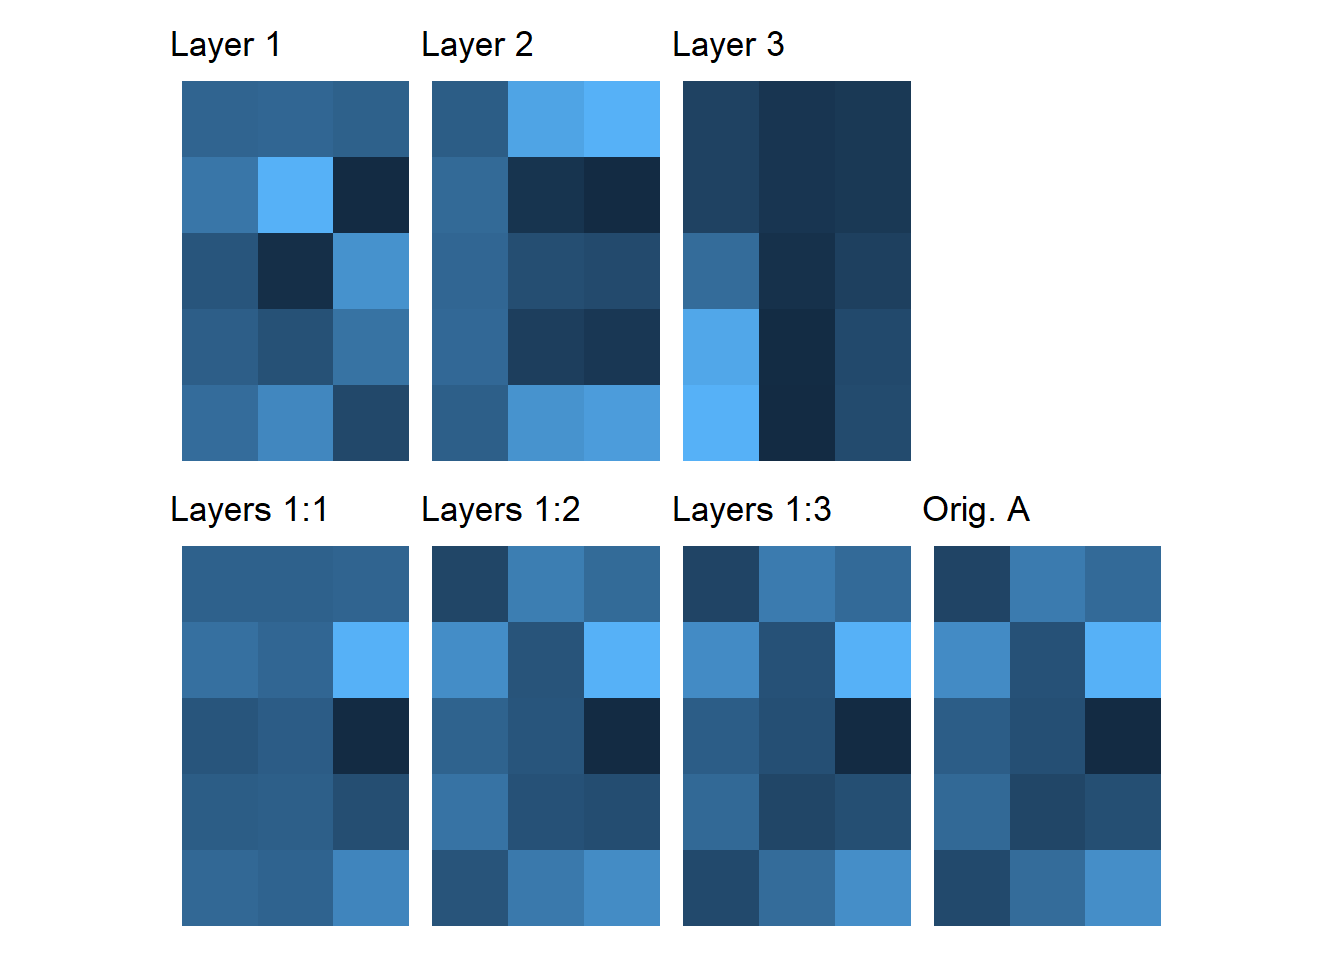
\includegraphics{cohen-linear-algebra_files/figure-latex/e16-3-1.pdf}

\hypertarget{exercise-4-2}{%
\subsection*{Exercise 4}\label{exercise-4-2}}
\addcontentsline{toc}{subsection}{Exercise 4}

\begin{Shaded}
\begin{Highlighting}[]
\NormalTok{m \textless{}{-}}\StringTok{ }\DecValTok{6}
\NormalTok{n \textless{}{-}}\StringTok{ }\DecValTok{16}
\NormalTok{condnum \textless{}{-}}\StringTok{ }\DecValTok{42}

\CommentTok{\# create U and V from random numbers}
\NormalTok{U \textless{}{-}}\StringTok{ }\KeywordTok{qr}\NormalTok{(}\KeywordTok{matrix}\NormalTok{(}\KeywordTok{rnorm}\NormalTok{(m}\OperatorTok{*}\NormalTok{m), }\DataTypeTok{nrow=}\NormalTok{m, }\DataTypeTok{ncol=}\NormalTok{m))}
\NormalTok{V \textless{}{-}}\StringTok{ }\KeywordTok{qr}\NormalTok{(}\KeywordTok{matrix}\NormalTok{(}\KeywordTok{rnorm}\NormalTok{(n}\OperatorTok{*}\NormalTok{n), }\DataTypeTok{nrow=}\NormalTok{n, }\DataTypeTok{ncol=}\NormalTok{n))}

\CommentTok{\# create singular values vector}
\NormalTok{s \textless{}{-}}\StringTok{ }\KeywordTok{seq}\NormalTok{(condnum, }\DecValTok{1}\NormalTok{, }\DataTypeTok{length.out =} \KeywordTok{min}\NormalTok{(}\KeywordTok{c}\NormalTok{(m,n)))}
\NormalTok{S \textless{}{-}}\StringTok{ }\KeywordTok{diag}\NormalTok{(s, }\DataTypeTok{nrow=}\NormalTok{m, }\DataTypeTok{ncol=}\NormalTok{n)}
\CommentTok{\# ↓ original code ↓}
\CommentTok{\# S \textless{}{-} matrix(0, nrow=m, ncol=n)}
\CommentTok{\# for(i in 1:min(c(m, n)))\{}
\CommentTok{\#   S[i, i] \textless{}{-} s[i]}
\CommentTok{\# \}}

\NormalTok{A \textless{}{-}}\StringTok{ }\KeywordTok{qr.Q}\NormalTok{(U) }\OperatorTok{\%*\%}\StringTok{ }\NormalTok{S }\OperatorTok{\%*\%}\StringTok{ }\KeywordTok{t}\NormalTok{(}\KeywordTok{qr.Q}\NormalTok{(V)) }\CommentTok{\# construct matrix}
\NormalTok{pracma}\OperatorTok{::}\KeywordTok{cond}\NormalTok{(A)}
\end{Highlighting}
\end{Shaded}

\begin{verbatim}
## [1] 42
\end{verbatim}

\hypertarget{exercise-5-1}{%
\subsection*{Exercise 5}\label{exercise-5-1}}
\addcontentsline{toc}{subsection}{Exercise 5}

\begin{Shaded}
\begin{Highlighting}[]
\KeywordTok{library}\NormalTok{(imager)}

\NormalTok{rankN \textless{}{-}}\StringTok{ }\DecValTok{20}

\NormalTok{picture \textless{}{-}}\StringTok{ }\NormalTok{imager}\OperatorTok{::}\KeywordTok{load.image}\NormalTok{(}\StringTok{\textquotesingle{}https://upload.wikimedia.org/wikipedia/en/8/86/Einstein\_tongue.jpg\textquotesingle{}}\NormalTok{)}

\NormalTok{pic \textless{}{-}}\StringTok{ }\KeywordTok{as.matrix}\NormalTok{(picture)}
\NormalTok{picSVD \textless{}{-}}\StringTok{ }\KeywordTok{svd}\NormalTok{(pic, }\DataTypeTok{nu=}\KeywordTok{nrow}\NormalTok{(pic), }\DataTypeTok{nv=}\KeywordTok{ncol}\NormalTok{(pic))}
\NormalTok{S \textless{}{-}}\StringTok{ }\KeywordTok{diag}\NormalTok{(picSVD}\OperatorTok{$}\NormalTok{d, }\DataTypeTok{nrow=}\KeywordTok{nrow}\NormalTok{(pic), }\DataTypeTok{ncol=}\KeywordTok{ncol}\NormalTok{(pic))}

\NormalTok{lowrank \textless{}{-}}\StringTok{ }\NormalTok{picSVD}\OperatorTok{$}\NormalTok{u[, }\DecValTok{1}\OperatorTok{:}\NormalTok{rankN] }\OperatorTok{\%*\%}\StringTok{ }\NormalTok{S[}\DecValTok{1}\OperatorTok{:}\NormalTok{rankN, }\DecValTok{1}\OperatorTok{:}\NormalTok{rankN] }\OperatorTok{\%*\%}\StringTok{ }\KeywordTok{t}\NormalTok{(picSVD}\OperatorTok{$}\NormalTok{v)[}\DecValTok{1}\OperatorTok{:}\NormalTok{rankN,]}

\KeywordTok{plot}\NormalTok{(imager}\OperatorTok{::}\KeywordTok{as.cimg}\NormalTok{(lowrank), }\DataTypeTok{axes=}\OtherTok{FALSE}\NormalTok{)}
\end{Highlighting}
\end{Shaded}

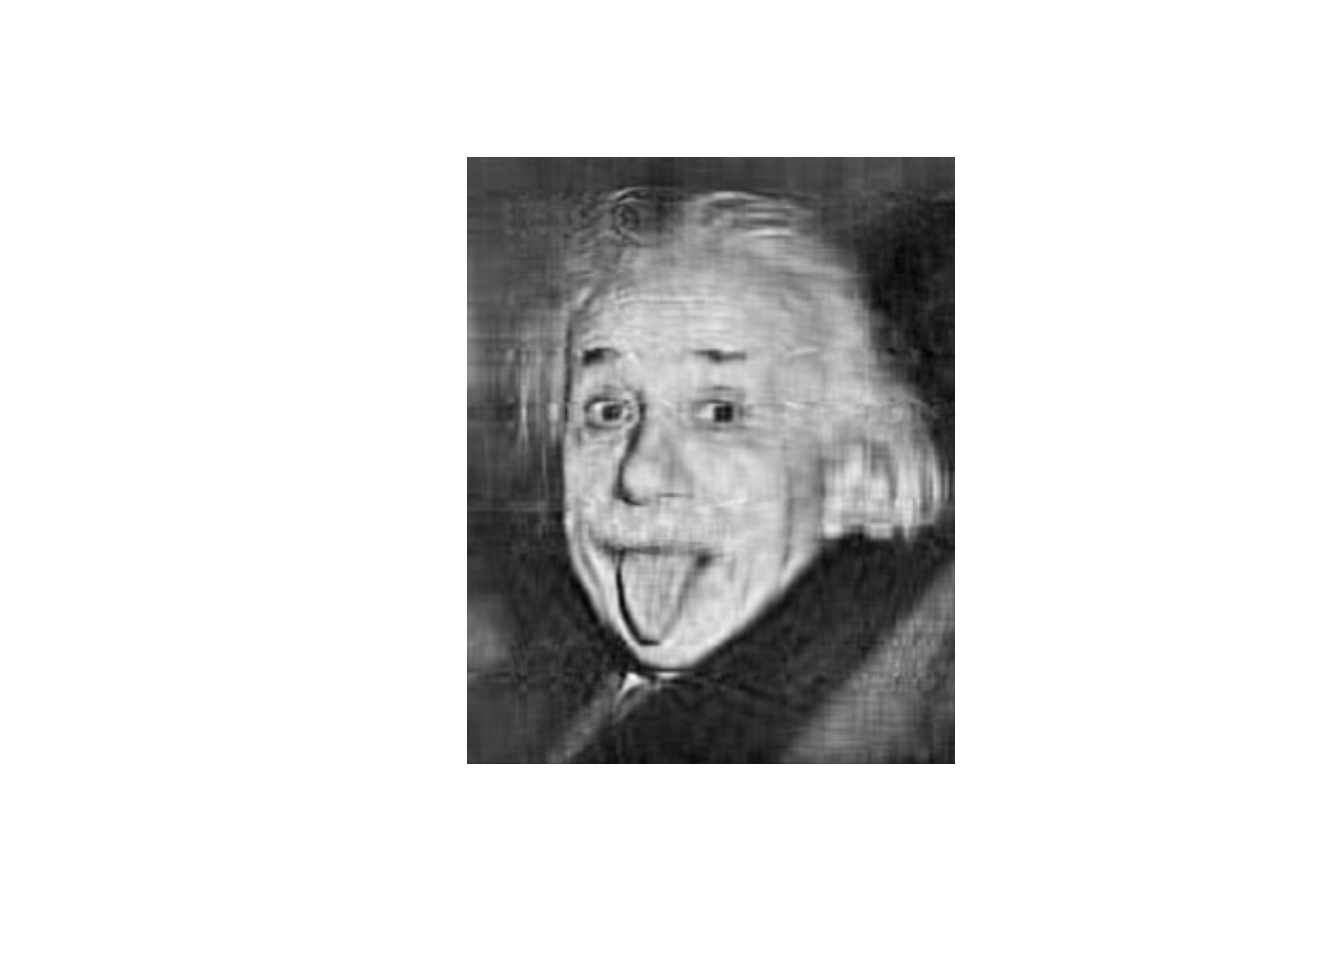
\includegraphics{cohen-linear-algebra_files/figure-latex/e16-5-1.pdf}

\hypertarget{exercise-6}{%
\subsection*{Exercise 6}\label{exercise-6}}
\addcontentsline{toc}{subsection}{Exercise 6}

\begin{Shaded}
\begin{Highlighting}[]
\KeywordTok{library}\NormalTok{(imager)}

\CommentTok{\# convert to percent explained}
\NormalTok{s \textless{}{-}}\StringTok{ }\DecValTok{100} \OperatorTok{*}\StringTok{ }\NormalTok{picSVD}\OperatorTok{$}\NormalTok{d }\OperatorTok{/}\StringTok{ }\KeywordTok{sum}\NormalTok{(picSVD}\OperatorTok{$}\NormalTok{d)}
\KeywordTok{ggplot}\NormalTok{(}\DataTypeTok{data=}\OtherTok{NULL}\NormalTok{, }\KeywordTok{aes}\NormalTok{(}\DataTypeTok{x=}\DecValTok{1}\OperatorTok{:}\DecValTok{100}\NormalTok{, }\DataTypeTok{y=}\NormalTok{s[}\DecValTok{1}\OperatorTok{:}\DecValTok{100}\NormalTok{])) }\OperatorTok{+}\StringTok{ }
\StringTok{  }\KeywordTok{geom\_line}\NormalTok{() }\OperatorTok{+}
\StringTok{  }\KeywordTok{geom\_point}\NormalTok{() }\OperatorTok{+}
\StringTok{  }\KeywordTok{xlab}\NormalTok{(}\StringTok{"Component number"}\NormalTok{) }\OperatorTok{+}
\StringTok{  }\KeywordTok{ylab}\NormalTok{(}\StringTok{"Pct variance explains"}\NormalTok{)}
\end{Highlighting}
\end{Shaded}

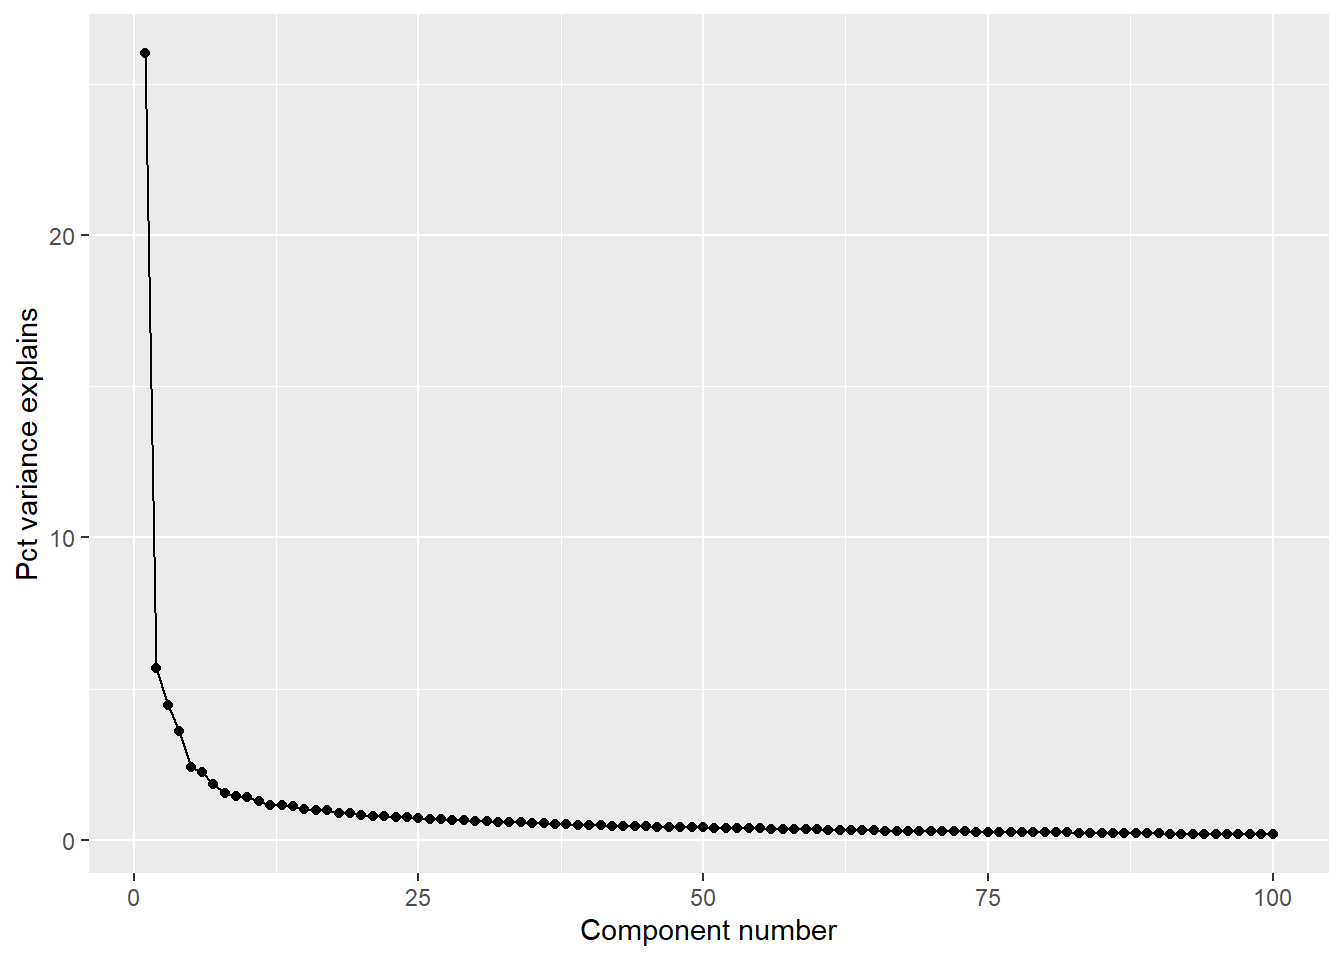
\includegraphics{cohen-linear-algebra_files/figure-latex/e16-6-1.pdf}

\begin{Shaded}
\begin{Highlighting}[]
\NormalTok{thresh \textless{}{-}}\StringTok{ }\DecValTok{4} \CommentTok{\# threshold in percent}
\NormalTok{comps \textless{}{-}}\StringTok{ }\NormalTok{s }\OperatorTok{\textgreater{}}\StringTok{ }\NormalTok{thresh }\CommentTok{\# comps greater than X\%}
\NormalTok{lowrank \textless{}{-}}\StringTok{ }\NormalTok{picSVD}\OperatorTok{$}\NormalTok{u[, comps] }\OperatorTok{\%*\%}\StringTok{ }\NormalTok{S[comps, comps] }\OperatorTok{\%*\%}\StringTok{ }\KeywordTok{t}\NormalTok{(picSVD}\OperatorTok{$}\NormalTok{v)[comps,]}

\KeywordTok{layout}\NormalTok{(}\KeywordTok{t}\NormalTok{(}\KeywordTok{c}\NormalTok{(}\DecValTok{1}\NormalTok{,}\DecValTok{2}\NormalTok{)))}
\KeywordTok{plot}\NormalTok{(picture, }\DataTypeTok{axes=}\OtherTok{FALSE}\NormalTok{, }\DataTypeTok{main=}\StringTok{"Original"}\NormalTok{)}
\KeywordTok{plot}\NormalTok{(}\KeywordTok{as.cimg}\NormalTok{(lowrank), }\DataTypeTok{axes=}\OtherTok{FALSE}\NormalTok{, }\DataTypeTok{main=}\KeywordTok{sprintf}\NormalTok{(}\StringTok{"\%s comps with \textgreater{} \%g\%\%"}\NormalTok{, }\KeywordTok{sum}\NormalTok{(comps), thresh))}
\end{Highlighting}
\end{Shaded}

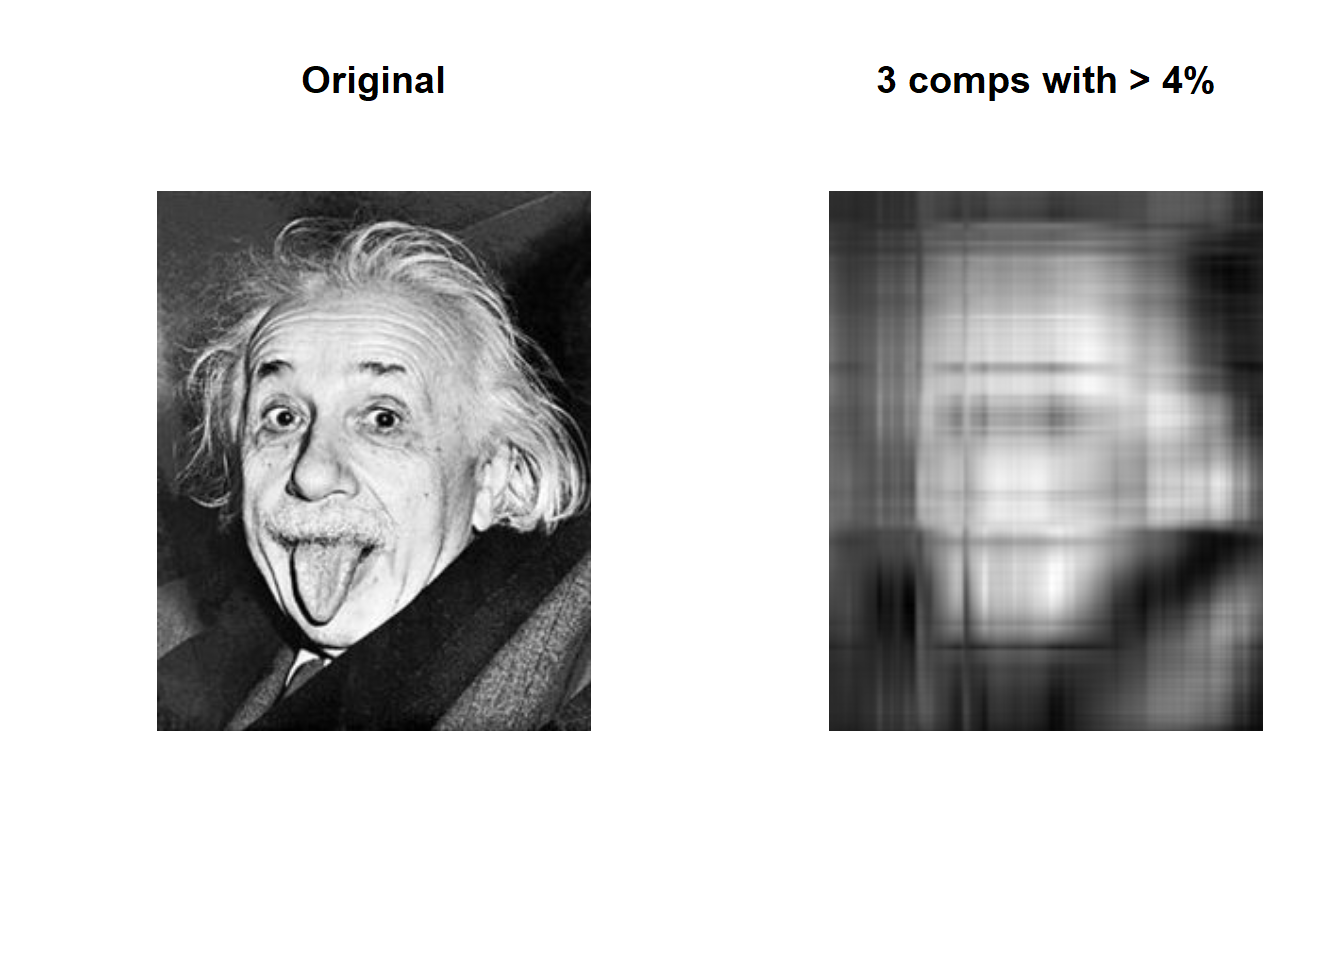
\includegraphics{cohen-linear-algebra_files/figure-latex/e16-6-2.pdf}

\hypertarget{exercise-7}{%
\subsection*{Exercise 7}\label{exercise-7}}
\addcontentsline{toc}{subsection}{Exercise 7}

Note \texttt{matrix(picSVD\$u{[},\ 1:si{]},\ ncol=si)}. Without \texttt{matrix(,\ ncol=si)}, \texttt{picSVD\$u{[},\ 1:si{]}} becomes an atomic vector and matrix multiplication breaks down.

\begin{Shaded}
\begin{Highlighting}[]
\KeywordTok{library}\NormalTok{(ggplot2)}

\NormalTok{RMS \textless{}{-}}\StringTok{ }\KeywordTok{rep}\NormalTok{(}\DecValTok{0}\NormalTok{, }\KeywordTok{length}\NormalTok{(s))}
\ControlFlowTok{for}\NormalTok{(si }\ControlFlowTok{in} \DecValTok{1}\OperatorTok{:}\KeywordTok{length}\NormalTok{(s))\{}
\NormalTok{  lowrank \textless{}{-}}\StringTok{ }\KeywordTok{matrix}\NormalTok{(picSVD}\OperatorTok{$}\NormalTok{u[, }\DecValTok{1}\OperatorTok{:}\NormalTok{si], }\DataTypeTok{ncol=}\NormalTok{si) }\OperatorTok{\%*\%}\StringTok{ }\NormalTok{S[}\DecValTok{1}\OperatorTok{:}\NormalTok{si, }\DecValTok{1}\OperatorTok{:}\NormalTok{si] }\OperatorTok{\%*\%}\StringTok{ }\KeywordTok{t}\NormalTok{(picSVD}\OperatorTok{$}\NormalTok{v)[}\DecValTok{1}\OperatorTok{:}\NormalTok{si,]}
\NormalTok{  diffimg \textless{}{-}}\StringTok{ }\NormalTok{lowrank }\OperatorTok{{-}}\StringTok{ }\NormalTok{pic}
\NormalTok{  RMS[si] \textless{}{-}}\StringTok{ }\KeywordTok{sqrt}\NormalTok{(}\KeywordTok{mean}\NormalTok{(diffimg}\OperatorTok{\^{}}\DecValTok{2}\NormalTok{))}
\NormalTok{\}}

\KeywordTok{ggplot}\NormalTok{(}\DataTypeTok{data=}\OtherTok{NULL}\NormalTok{, }\KeywordTok{aes}\NormalTok{(}\DataTypeTok{x=}\DecValTok{1}\OperatorTok{:}\KeywordTok{length}\NormalTok{(RMS), }\DataTypeTok{y=}\NormalTok{RMS)) }\OperatorTok{+}\StringTok{ }
\StringTok{  }\KeywordTok{geom\_line}\NormalTok{() }\OperatorTok{+}\StringTok{ }
\StringTok{  }\KeywordTok{xlab}\NormalTok{(}\StringTok{"Rank approximation"}\NormalTok{) }\OperatorTok{+}\StringTok{ }
\StringTok{  }\KeywordTok{ylab}\NormalTok{(}\StringTok{"Error (a.u.)"}\NormalTok{)}
\end{Highlighting}
\end{Shaded}

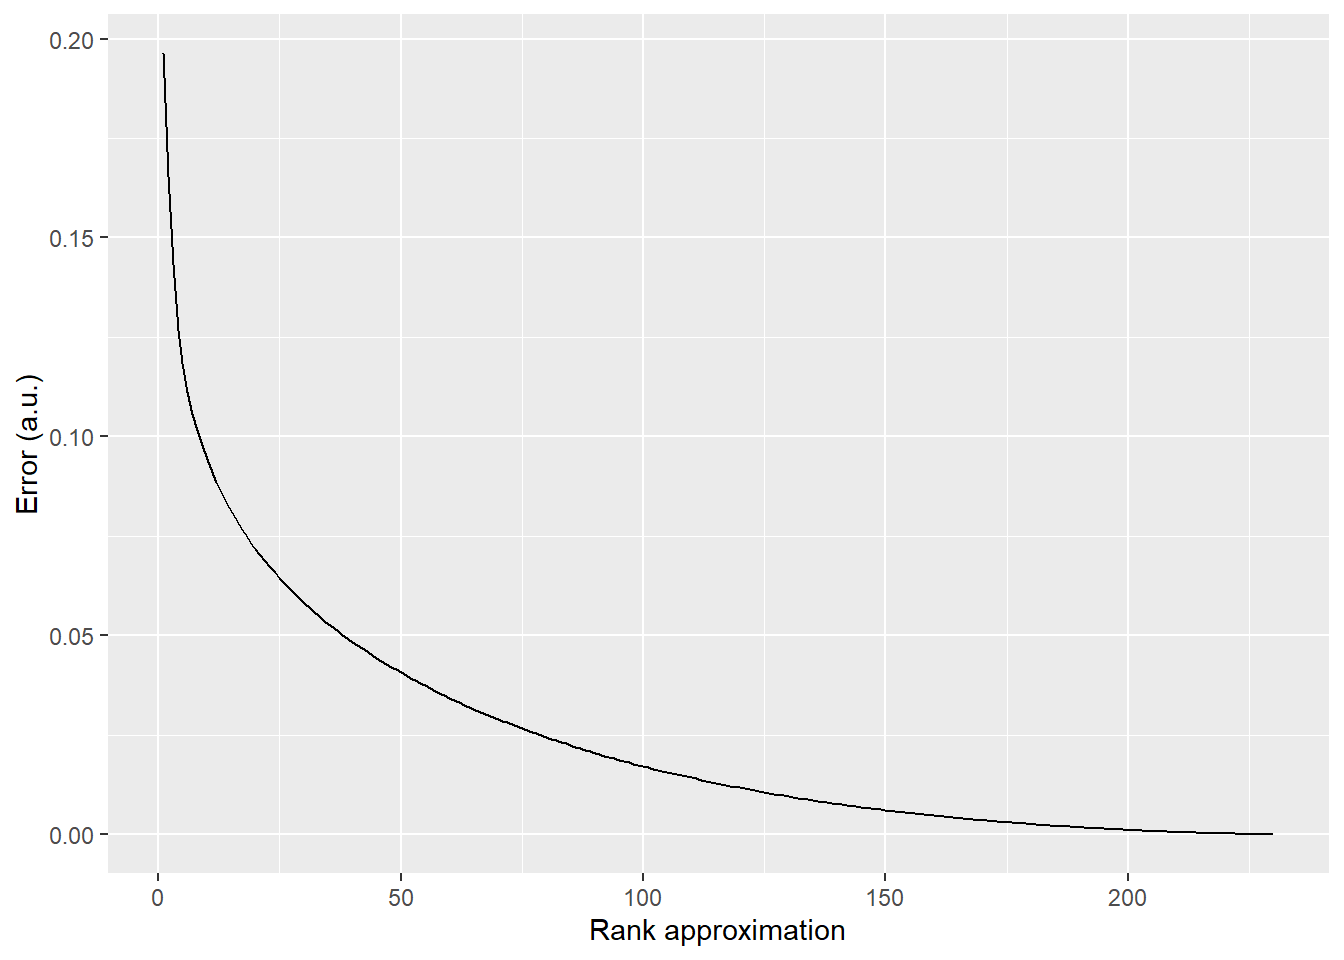
\includegraphics{cohen-linear-algebra_files/figure-latex/e16-7-1.pdf}

\hypertarget{exercise-8}{%
\subsection*{Exercise 8}\label{exercise-8}}
\addcontentsline{toc}{subsection}{Exercise 8}

Reminder, you need to specify \texttt{nu} and \texttt{nv} to ensure full matrices U and V.

\begin{Shaded}
\begin{Highlighting}[]
\KeywordTok{library}\NormalTok{(matrixcalc)}

\NormalTok{X \textless{}{-}}\StringTok{ }\KeywordTok{matrix}\NormalTok{(}\KeywordTok{sample}\NormalTok{(}\DecValTok{1}\OperatorTok{:}\DecValTok{6}\NormalTok{, }\DataTypeTok{size =} \DecValTok{4}\OperatorTok{*}\DecValTok{2}\NormalTok{, }\DataTypeTok{replace =} \OtherTok{TRUE}\NormalTok{), }\DataTypeTok{nrow=}\DecValTok{4}\NormalTok{, }\DataTypeTok{ncol=}\DecValTok{2}\NormalTok{)}
\NormalTok{svdX \textless{}{-}}\StringTok{ }\KeywordTok{svd}\NormalTok{(X, }\DataTypeTok{nu=}\KeywordTok{nrow}\NormalTok{(X), }\DataTypeTok{nv=}\KeywordTok{ncol}\NormalTok{(X)) }\CommentTok{\# eq. 29}
\NormalTok{U \textless{}{-}}\StringTok{ }\NormalTok{svdX}\OperatorTok{$}\NormalTok{u}
\NormalTok{S \textless{}{-}}\StringTok{ }\KeywordTok{diag}\NormalTok{(svdX}\OperatorTok{$}\NormalTok{d, }\DataTypeTok{nrow=}\KeywordTok{nrow}\NormalTok{(X), }\DataTypeTok{ncol=}\KeywordTok{ncol}\NormalTok{(X))}
\NormalTok{V \textless{}{-}}\StringTok{ }\NormalTok{svdX}\OperatorTok{$}\NormalTok{v}

\NormalTok{longV1 \textless{}{-}}\StringTok{ }\KeywordTok{solve}\NormalTok{(}\KeywordTok{t}\NormalTok{(U}\OperatorTok{\%*\%}\NormalTok{S}\OperatorTok{\%*\%}\KeywordTok{t}\NormalTok{(V))}\OperatorTok{\%*\%}\NormalTok{U}\OperatorTok{\%*\%}\NormalTok{S}\OperatorTok{\%*\%}\KeywordTok{t}\NormalTok{(V)) }\OperatorTok{\%*\%}\StringTok{ }\KeywordTok{t}\NormalTok{(U}\OperatorTok{\%*\%}\NormalTok{S}\OperatorTok{\%*\%}\KeywordTok{t}\NormalTok{(V)) }\CommentTok{\# eq. 30}
\NormalTok{longV2 \textless{}{-}}\StringTok{ }\KeywordTok{solve}\NormalTok{(V}\OperatorTok{\%*\%}\KeywordTok{t}\NormalTok{(S)}\OperatorTok{\%*\%}\KeywordTok{t}\NormalTok{(U)}\OperatorTok{\%*\%}\NormalTok{U}\OperatorTok{\%*\%}\NormalTok{S}\OperatorTok{\%*\%}\KeywordTok{t}\NormalTok{(V)) }\OperatorTok{\%*\%}\StringTok{ }\KeywordTok{t}\NormalTok{(U}\OperatorTok{\%*\%}\NormalTok{S}\OperatorTok{\%*\%}\KeywordTok{t}\NormalTok{(V)) }\CommentTok{\# eq. 31}
\NormalTok{longV3 \textless{}{-}}\StringTok{ }\KeywordTok{solve}\NormalTok{(V}\OperatorTok{\%*\%}\KeywordTok{t}\NormalTok{(S)}\OperatorTok{\%*\%}\NormalTok{S}\OperatorTok{\%*\%}\KeywordTok{t}\NormalTok{(V)) }\OperatorTok{\%*\%}\StringTok{ }\KeywordTok{t}\NormalTok{(U}\OperatorTok{\%*\%}\NormalTok{S}\OperatorTok{\%*\%}\KeywordTok{t}\NormalTok{(V)) }\CommentTok{\# eq. 32}
\NormalTok{longV4 \textless{}{-}}\StringTok{ }\NormalTok{V }\OperatorTok{\%*\%}\StringTok{ }\NormalTok{matrixcalc}\OperatorTok{::}\KeywordTok{matrix.power}\NormalTok{(}\KeywordTok{t}\NormalTok{(S) }\OperatorTok{\%*\%}\StringTok{ }\NormalTok{S, }\DecValTok{{-}1}\NormalTok{) }\OperatorTok{\%*\%}\StringTok{ }\KeywordTok{t}\NormalTok{(V)}\OperatorTok{\%*\%}\NormalTok{V}\OperatorTok{\%*\%}\KeywordTok{t}\NormalTok{(S)}\OperatorTok{\%*\%}\KeywordTok{t}\NormalTok{(U) }\CommentTok{\# eq. 33 }

\NormalTok{MPpinv \textless{}{-}}\StringTok{ }\NormalTok{pracma}\OperatorTok{::}\KeywordTok{pinv}\NormalTok{(X) }\CommentTok{\# eq. 34}
\end{Highlighting}
\end{Shaded}

\hypertarget{exercise-9}{%
\subsection*{Exercise 9}\label{exercise-9}}
\addcontentsline{toc}{subsection}{Exercise 9}

\begin{Shaded}
\begin{Highlighting}[]
\NormalTok{k \textless{}{-}}\StringTok{ }\DecValTok{5}
\NormalTok{n \textless{}{-}}\StringTok{ }\DecValTok{13}
\NormalTok{a \textless{}{-}}\StringTok{ }\NormalTok{pracma}\OperatorTok{::}\KeywordTok{pinv}\NormalTok{(}\KeywordTok{matrix}\NormalTok{(}\DecValTok{1}\NormalTok{, }\DataTypeTok{nrow=}\NormalTok{n, }\DataTypeTok{ncol=}\DecValTok{1}\NormalTok{) }\OperatorTok{*}\StringTok{ }\NormalTok{k)}
\NormalTok{a }\OperatorTok{{-}}\StringTok{ }\DecValTok{1} \OperatorTok{/}\StringTok{ }\NormalTok{(k }\OperatorTok{*}\StringTok{ }\NormalTok{n) }\CommentTok{\# check for zeros}
\end{Highlighting}
\end{Shaded}

\begin{verbatim}
##              [,1]         [,2]         [,3]         [,4]         [,5]
## [1,] 8.673617e-18 6.938894e-18 6.938894e-18 6.938894e-18 6.938894e-18
##              [,6]         [,7]         [,8]         [,9]        [,10]
## [1,] 6.938894e-18 6.938894e-18 6.938894e-18 6.938894e-18 6.938894e-18
##             [,11]        [,12]        [,13]
## [1,] 6.938894e-18 6.938894e-18 6.938894e-18
\end{verbatim}

\hypertarget{exercise-10}{%
\subsection*{Exercise 10}\label{exercise-10}}
\addcontentsline{toc}{subsection}{Exercise 10}

\begin{Shaded}
\begin{Highlighting}[]
\NormalTok{M \textless{}{-}}\StringTok{ }\DecValTok{10}
\NormalTok{cns \textless{}{-}}\StringTok{ }\KeywordTok{seq}\NormalTok{(}\DecValTok{10}\NormalTok{, }\FloatTok{1e10}\NormalTok{, }\DataTypeTok{length.out=}\DecValTok{30}\NormalTok{)}
\NormalTok{avediffs \textless{}{-}}\StringTok{ }\KeywordTok{rep}\NormalTok{(}\DecValTok{0}\NormalTok{, }\KeywordTok{length}\NormalTok{(cns))}

\CommentTok{\# loop over condition numbers  }
\ControlFlowTok{for}\NormalTok{(condi }\ControlFlowTok{in} \DecValTok{1}\OperatorTok{:}\KeywordTok{length}\NormalTok{(cns))\{}
  \CommentTok{\# create A}
\NormalTok{  U \textless{}{-}}\StringTok{ }\KeywordTok{qr.Q}\NormalTok{(}\KeywordTok{qr}\NormalTok{(}\KeywordTok{matrix}\NormalTok{(}\KeywordTok{rnorm}\NormalTok{(M}\OperatorTok{\^{}}\DecValTok{2}\NormalTok{), }\DataTypeTok{nrow=}\NormalTok{M, }\DataTypeTok{ncol=}\NormalTok{M)))}
\NormalTok{  V \textless{}{-}}\StringTok{ }\KeywordTok{qr.Q}\NormalTok{(}\KeywordTok{qr}\NormalTok{(}\KeywordTok{matrix}\NormalTok{(}\KeywordTok{rnorm}\NormalTok{(M}\OperatorTok{\^{}}\DecValTok{2}\NormalTok{), }\DataTypeTok{nrow=}\NormalTok{M, }\DataTypeTok{ncol=}\NormalTok{M)))}
\NormalTok{  S \textless{}{-}}\StringTok{ }\KeywordTok{diag}\NormalTok{(cns[condi], }\DataTypeTok{nrow=}\NormalTok{M, }\DataTypeTok{ncol=}\NormalTok{M)}
\NormalTok{  A \textless{}{-}}\StringTok{ }\NormalTok{U }\OperatorTok{\%*\%}\StringTok{ }\NormalTok{S }\OperatorTok{\%*\%}\StringTok{ }\KeywordTok{t}\NormalTok{(V) }\CommentTok{\# construct matrix }

  \CommentTok{\# create B}
\NormalTok{  U \textless{}{-}}\StringTok{ }\KeywordTok{qr.Q}\NormalTok{(}\KeywordTok{qr}\NormalTok{(}\KeywordTok{matrix}\NormalTok{(}\KeywordTok{rnorm}\NormalTok{(M}\OperatorTok{\^{}}\DecValTok{2}\NormalTok{), }\DataTypeTok{nrow=}\NormalTok{M, }\DataTypeTok{ncol=}\NormalTok{M)))}
\NormalTok{  V \textless{}{-}}\StringTok{ }\KeywordTok{qr.Q}\NormalTok{(}\KeywordTok{qr}\NormalTok{(}\KeywordTok{matrix}\NormalTok{(}\KeywordTok{rnorm}\NormalTok{(M}\OperatorTok{\^{}}\DecValTok{2}\NormalTok{), }\DataTypeTok{nrow=}\NormalTok{M, }\DataTypeTok{ncol=}\NormalTok{M)))}
\NormalTok{  S \textless{}{-}}\StringTok{ }\KeywordTok{diag}\NormalTok{(cns[condi], }\DataTypeTok{nrow=}\NormalTok{M, }\DataTypeTok{ncol=}\NormalTok{M)}
\NormalTok{  B \textless{}{-}}\StringTok{ }\NormalTok{U }\OperatorTok{\%*\%}\StringTok{ }\NormalTok{S }\OperatorTok{\%*\%}\StringTok{ }\KeywordTok{t}\NormalTok{(V) }\CommentTok{\# construct matrix }
  
  \CommentTok{\# GEDs and sort}
\NormalTok{  l1 \textless{}{-}}\StringTok{ }\KeywordTok{sort}\NormalTok{(}\KeywordTok{eigen}\NormalTok{(A)}\OperatorTok{$}\NormalTok{values)}
\NormalTok{  l2 \textless{}{-}}\StringTok{ }\KeywordTok{sort}\NormalTok{(}\KeywordTok{eigen}\NormalTok{(B)}\OperatorTok{$}\NormalTok{values)}
  
\NormalTok{  avediffs[condi] \textless{}{-}}\StringTok{ }\KeywordTok{mean}\NormalTok{(}\KeywordTok{abs}\NormalTok{(l1}\OperatorTok{{-}}\NormalTok{l2))}
\NormalTok{\}}

\KeywordTok{ggplot}\NormalTok{(}\DataTypeTok{data=}\OtherTok{NULL}\NormalTok{, }\KeywordTok{aes}\NormalTok{(}\DataTypeTok{x=}\NormalTok{cns, }\DataTypeTok{y=}\NormalTok{avediffs)) }\OperatorTok{+}\StringTok{ }
\StringTok{  }\KeywordTok{geom\_line}\NormalTok{() }\OperatorTok{+}\StringTok{ }
\StringTok{  }\KeywordTok{xlab}\NormalTok{(}\StringTok{"Cond. number"}\NormalTok{) }\OperatorTok{+}\StringTok{ }
\StringTok{  }\KeywordTok{ylab}\NormalTok{(}\KeywordTok{expression}\NormalTok{(}\KeywordTok{paste}\NormalTok{(Delta, lamda)))}
\end{Highlighting}
\end{Shaded}

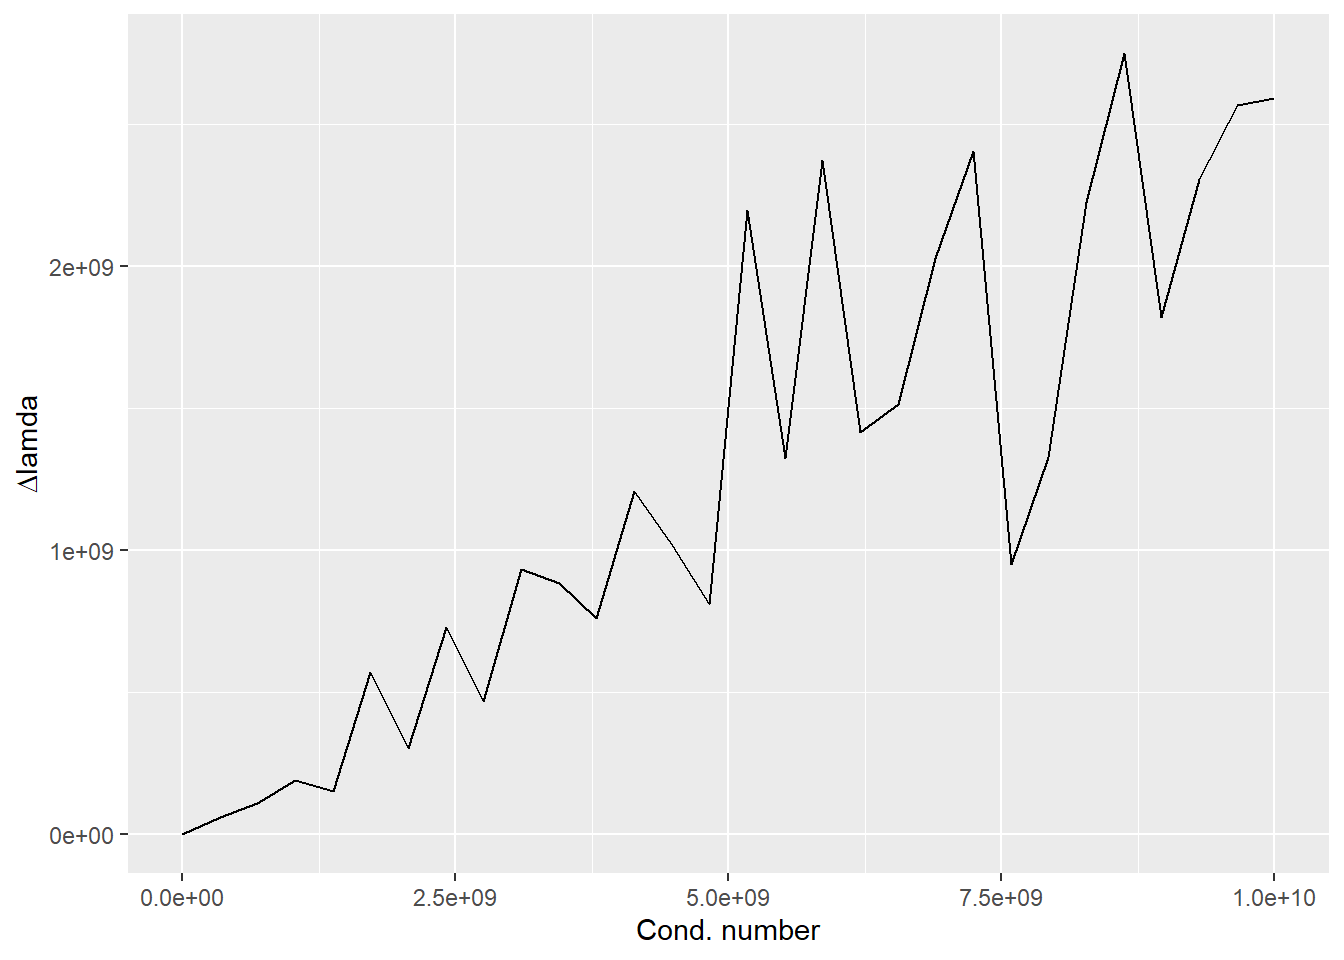
\includegraphics{cohen-linear-algebra_files/figure-latex/e16-10-1.pdf}
\#\# Chapter 17
\#\#\# Exercise 1 \{-\}

\begin{Shaded}
\begin{Highlighting}[]
\KeywordTok{library}\NormalTok{(plotly)}

\NormalTok{A \textless{}{-}}\StringTok{ }\KeywordTok{matrix}\NormalTok{(}\KeywordTok{c}\NormalTok{(}\OperatorTok{{-}}\DecValTok{2}\NormalTok{, }\DecValTok{3}\NormalTok{, }\DecValTok{2}\NormalTok{, }\DecValTok{8}\NormalTok{), }\DataTypeTok{nrow=}\DecValTok{2}\NormalTok{, }\DataTypeTok{ncol=}\DecValTok{2}\NormalTok{, }\DataTypeTok{byrow=}\OtherTok{TRUE}\NormalTok{)}
\NormalTok{vi \textless{}{-}}\StringTok{ }\KeywordTok{seq}\NormalTok{(}\OperatorTok{{-}}\DecValTok{2}\NormalTok{, }\DecValTok{2}\NormalTok{, }\DataTypeTok{step=}\FloatTok{0.1}\NormalTok{)}
\NormalTok{quadform \textless{}{-}}\StringTok{ }\KeywordTok{matrix}\NormalTok{(}\DecValTok{0}\NormalTok{, }\DataTypeTok{nrow=}\KeywordTok{length}\NormalTok{(vi), }\DataTypeTok{ncol=}\KeywordTok{length}\NormalTok{(vi))}

\ControlFlowTok{for}\NormalTok{(i }\ControlFlowTok{in} \DecValTok{1}\OperatorTok{:}\KeywordTok{length}\NormalTok{(vi))\{}
  \ControlFlowTok{for}\NormalTok{(j }\ControlFlowTok{in} \DecValTok{1}\OperatorTok{:}\KeywordTok{length}\NormalTok{(vi))\{}
\NormalTok{    v \textless{}{-}}\StringTok{ }\KeywordTok{matrix}\NormalTok{(}\KeywordTok{c}\NormalTok{(vi[i], vi[j]), }\DataTypeTok{ncol=}\DecValTok{1}\NormalTok{)}
\NormalTok{    quadform[i, j] \textless{}{-}}\StringTok{ }\KeywordTok{t}\NormalTok{(v) }\OperatorTok{\%*\%}\StringTok{ }\NormalTok{A }\OperatorTok{\%*\%}\StringTok{ }\NormalTok{v }\OperatorTok{/}\StringTok{ }\NormalTok{(}\KeywordTok{t}\NormalTok{(v) }\OperatorTok{\%*\%}\StringTok{ }\NormalTok{v)}
\NormalTok{  \}}
\NormalTok{\}}
  
\KeywordTok{plot\_ly}\NormalTok{(}\DataTypeTok{z =}\NormalTok{ quadform, }\DataTypeTok{type =} \StringTok{"surface"}\NormalTok{)}
\end{Highlighting}
\end{Shaded}


\includegraphics[width=26.39in]{images/e17-1}

\hypertarget{exercise-2-12}{%
\subsection*{Exercise 2}\label{exercise-2-12}}
\addcontentsline{toc}{subsection}{Exercise 2}

\begin{Shaded}
\begin{Highlighting}[]
\NormalTok{n \textless{}{-}}\StringTok{ }\DecValTok{4}
\NormalTok{nIterations \textless{}{-}}\StringTok{ }\DecValTok{500}
\NormalTok{defcat \textless{}{-}}\StringTok{ }\KeywordTok{rep}\NormalTok{(}\DecValTok{0}\NormalTok{, nIterations)}

\ControlFlowTok{for}\NormalTok{(iteri }\ControlFlowTok{in} \DecValTok{1}\OperatorTok{:}\NormalTok{nIterations)\{}
  \CommentTok{\# create matrix}
\NormalTok{  A \textless{}{-}}\StringTok{ }\KeywordTok{matrix}\NormalTok{(}\KeywordTok{sample}\NormalTok{(}\OperatorTok{{-}}\DecValTok{10}\OperatorTok{:}\DecValTok{10}\NormalTok{, }\DataTypeTok{size=}\NormalTok{n}\OperatorTok{\^{}}\DecValTok{2}\NormalTok{, }\DataTypeTok{replace=}\OtherTok{TRUE}\NormalTok{), }\DataTypeTok{nrow=}\NormalTok{n, }\DataTypeTok{ncol=}\NormalTok{n)}
\NormalTok{  e \textless{}{-}}\StringTok{ }\KeywordTok{eigen}\NormalTok{(A)}\OperatorTok{$}\NormalTok{values}
  \ControlFlowTok{while}\NormalTok{ (}\KeywordTok{is.complex}\NormalTok{(e))\{}
\NormalTok{    A \textless{}{-}}\StringTok{ }\KeywordTok{matrix}\NormalTok{(}\KeywordTok{sample}\NormalTok{(}\OperatorTok{{-}}\DecValTok{10}\OperatorTok{:}\DecValTok{10}\NormalTok{, }\DataTypeTok{size=}\NormalTok{n}\OperatorTok{\^{}}\DecValTok{2}\NormalTok{, }\DataTypeTok{replace=}\OtherTok{TRUE}\NormalTok{), }\DataTypeTok{nrow=}\NormalTok{n, }\DataTypeTok{ncol=}\NormalTok{n)}
\NormalTok{    e \textless{}{-}}\StringTok{ }\KeywordTok{eigen}\NormalTok{(A)}\OperatorTok{$}\NormalTok{values}
\NormalTok{  \}}
  
  \CommentTok{\# "zero" threshold (from rank)}
\NormalTok{  t \textless{}{-}}\StringTok{ }\NormalTok{n }\OperatorTok{*}\StringTok{ }\NormalTok{pracma}\OperatorTok{::}\KeywordTok{eps}\NormalTok{(}\KeywordTok{max}\NormalTok{(}\KeywordTok{svd}\NormalTok{(A)}\OperatorTok{$}\NormalTok{d))}
  
  \CommentTok{\# test definiteness}
  \ControlFlowTok{if}\NormalTok{ (}\KeywordTok{all}\NormalTok{(}\KeywordTok{sign}\NormalTok{(e) }\OperatorTok{==}\StringTok{ }\DecValTok{1}\NormalTok{)) \{}
\NormalTok{    defcat[iteri] \textless{}{-}}\StringTok{ }\DecValTok{1} \CommentTok{\# pos. def}
\NormalTok{  \}}
  \ControlFlowTok{else} \ControlFlowTok{if}\NormalTok{ (}\KeywordTok{all}\NormalTok{(}\KeywordTok{sign}\NormalTok{(e)}\OperatorTok{\textgreater{}{-}}\DecValTok{1} \OperatorTok{\&}\StringTok{ }\NormalTok{(}\KeywordTok{sum}\NormalTok{(}\KeywordTok{abs}\NormalTok{(e)}\OperatorTok{\textless{}}\NormalTok{t)}\OperatorTok{\textgreater{}}\DecValTok{0}\NormalTok{)))\{}
\NormalTok{    defcat[iteri] \textless{}{-}}\StringTok{ }\DecValTok{2} \CommentTok{\# pos. semidef}
\NormalTok{  \}}
  \ControlFlowTok{else} \ControlFlowTok{if}\NormalTok{ (}\KeywordTok{all}\NormalTok{(}\KeywordTok{sign}\NormalTok{(e)}\OperatorTok{\textless{}}\DecValTok{1} \OperatorTok{\&}\StringTok{ }\NormalTok{(}\KeywordTok{sum}\NormalTok{(}\KeywordTok{abs}\NormalTok{(e)}\OperatorTok{\textless{}}\NormalTok{t)}\OperatorTok{\textgreater{}}\DecValTok{0}\NormalTok{)))\{}
\NormalTok{    defcat[iteri] \textless{}{-}}\StringTok{ }\DecValTok{4} \CommentTok{\# neg. semidef}
\NormalTok{  \}}
  \ControlFlowTok{else} \ControlFlowTok{if}\NormalTok{ (}\KeywordTok{all}\NormalTok{(}\KeywordTok{sign}\NormalTok{(e) }\OperatorTok{==}\StringTok{ }\DecValTok{{-}1}\NormalTok{)) \{}
\NormalTok{    defcat[iteri] \textless{}{-}}\StringTok{ }\DecValTok{5} \CommentTok{\# neg. def}
\NormalTok{  \}}
  \ControlFlowTok{else}\NormalTok{ \{}
\NormalTok{    defcat[iteri] \textless{}{-}}\StringTok{ }\DecValTok{3} \CommentTok{\# indefinite}
\NormalTok{  \}}
\NormalTok{\}}

\CommentTok{\# print out summary}
\ControlFlowTok{for}\NormalTok{(i }\ControlFlowTok{in} \DecValTok{1}\OperatorTok{:}\DecValTok{5}\NormalTok{)}
\NormalTok{\{}
  \KeywordTok{print}\NormalTok{(}\KeywordTok{sprintf}\NormalTok{(}\StringTok{"cat \%d: \%d"}\NormalTok{, i, }\KeywordTok{sum}\NormalTok{(defcat }\OperatorTok{==}\StringTok{ }\NormalTok{i)))}
\NormalTok{\}}
\end{Highlighting}
\end{Shaded}

\begin{verbatim}
## [1] "cat 1: 1"
## [1] "cat 2: 0"
## [1] "cat 3: 499"
## [1] "cat 4: 0"
## [1] "cat 5: 0"
\end{verbatim}

\hypertarget{chapter-18}{%
\section*{Chapter 18}\label{chapter-18}}
\addcontentsline{toc}{section}{Chapter 18}

\hypertarget{exercise-1-11}{%
\subsection*{Exercise 1}\label{exercise-1-11}}
\addcontentsline{toc}{subsection}{Exercise 1}

\begin{Shaded}
\begin{Highlighting}[]
\NormalTok{n \textless{}{-}}\StringTok{ }\DecValTok{200}
\NormalTok{X \textless{}{-}}\StringTok{ }\KeywordTok{matrix}\NormalTok{(}\KeywordTok{rnorm}\NormalTok{(n}\OperatorTok{*}\DecValTok{4}\NormalTok{), }\DataTypeTok{nrow=}\NormalTok{n, }\DataTypeTok{ncol=}\DecValTok{4}\NormalTok{) }\CommentTok{\# data}
\NormalTok{X \textless{}{-}}\StringTok{ }\KeywordTok{apply}\NormalTok{(X, }\DataTypeTok{MARGIN=}\DecValTok{2}\NormalTok{, }\DataTypeTok{FUN=}\NormalTok{scale, }\DataTypeTok{scale=}\OtherTok{FALSE}\NormalTok{) }\CommentTok{\# mean{-}center}
\NormalTok{covM \textless{}{-}}\StringTok{ }\KeywordTok{t}\NormalTok{(X) }\OperatorTok{\%*\%}\StringTok{ }\NormalTok{X }\OperatorTok{/}\StringTok{ }\NormalTok{(n}\DecValTok{{-}1}\NormalTok{) }\CommentTok{\# covariance}
\NormalTok{stdM \textless{}{-}}\StringTok{ }\KeywordTok{solve}\NormalTok{(}\KeywordTok{diag}\NormalTok{(}\KeywordTok{apply}\NormalTok{(X, }\DataTypeTok{MARGIN=}\DecValTok{2}\NormalTok{, }\DataTypeTok{FUN=}\NormalTok{sd))) }\CommentTok{\# stdevs}
\NormalTok{corM \textless{}{-}}\StringTok{ }\NormalTok{stdM }\OperatorTok{\%*\%}\StringTok{ }\KeywordTok{t}\NormalTok{(X) }\OperatorTok{\%*\%}\StringTok{ }\NormalTok{X }\OperatorTok{\%*\%}\StringTok{ }\NormalTok{stdM }\OperatorTok{/}\StringTok{ }\NormalTok{(n }\OperatorTok{{-}}\StringTok{ }\DecValTok{1}\NormalTok{) }\CommentTok{\# R}

\CommentTok{\# compare ours against R\textquotesingle{}s}
\KeywordTok{print}\NormalTok{(}\KeywordTok{round}\NormalTok{(covM }\OperatorTok{{-}}\StringTok{ }\KeywordTok{cov}\NormalTok{(X), }\DecValTok{3}\NormalTok{))}
\end{Highlighting}
\end{Shaded}

\begin{verbatim}
##      [,1] [,2] [,3] [,4]
## [1,]    0    0    0    0
## [2,]    0    0    0    0
## [3,]    0    0    0    0
## [4,]    0    0    0    0
\end{verbatim}

\begin{Shaded}
\begin{Highlighting}[]
\KeywordTok{print}\NormalTok{(}\KeywordTok{round}\NormalTok{(corM }\OperatorTok{{-}}\StringTok{ }\KeywordTok{cor}\NormalTok{(X), }\DecValTok{3}\NormalTok{))}
\end{Highlighting}
\end{Shaded}

\begin{verbatim}
##      [,1] [,2] [,3] [,4]
## [1,]    0    0    0    0
## [2,]    0    0    0    0
## [3,]    0    0    0    0
## [4,]    0    0    0    0
\end{verbatim}

\hypertarget{chapter-19}{%
\section*{Chapter 19}\label{chapter-19}}
\addcontentsline{toc}{section}{Chapter 19}

\hypertarget{exercise-1-12}{%
\subsection*{Exercise 1}\label{exercise-1-12}}
\addcontentsline{toc}{subsection}{Exercise 1}

\begin{Shaded}
\begin{Highlighting}[]
\KeywordTok{library}\NormalTok{(ggplot2)}

\CommentTok{\# create data}
\NormalTok{N \textless{}{-}}\StringTok{ }\DecValTok{1000}
\NormalTok{h \textless{}{-}}\StringTok{ }\KeywordTok{rnorm}\NormalTok{(}\DataTypeTok{n=}\NormalTok{N, }\DataTypeTok{mean =} \KeywordTok{seq}\NormalTok{(}\DecValTok{150}\NormalTok{, }\DecValTok{190}\NormalTok{, }\DataTypeTok{length.out =}\NormalTok{ N), }\DataTypeTok{sd=}\DecValTok{5}\NormalTok{)}
\NormalTok{w \textless{}{-}}\StringTok{ }\NormalTok{h }\OperatorTok{*}\StringTok{ }\FloatTok{.7} \OperatorTok{{-}}\StringTok{ }\DecValTok{50} \OperatorTok{+}\StringTok{ }\KeywordTok{rnorm}\NormalTok{(N, }\DataTypeTok{mean=}\DecValTok{0}\NormalTok{, }\DataTypeTok{sd=}\DecValTok{10}\NormalTok{)}

\CommentTok{\# covariance}
\NormalTok{X \textless{}{-}}\StringTok{ }\KeywordTok{cbind}\NormalTok{(h, w)}
\NormalTok{X \textless{}{-}}\StringTok{ }\KeywordTok{apply}\NormalTok{(X, }\DataTypeTok{MARGIN=}\DecValTok{2}\NormalTok{, scale, }\DataTypeTok{scale=}\OtherTok{FALSE}\NormalTok{)}
\NormalTok{C \textless{}{-}}\StringTok{ }\KeywordTok{t}\NormalTok{(X) }\OperatorTok{\%*\%}\StringTok{ }\NormalTok{X }\OperatorTok{/}\StringTok{ }\NormalTok{(}\KeywordTok{length}\NormalTok{(h) }\OperatorTok{{-}}\StringTok{ }\DecValTok{1}\NormalTok{)}

\CommentTok{\# PCA}
\NormalTok{eigC \textless{}{-}}\StringTok{ }\KeywordTok{eigen}\NormalTok{(C)}

\CommentTok{\# sorting below is redundant in R, as values and vectors are presorted}
\NormalTok{i \textless{}{-}}\StringTok{ }\KeywordTok{order}\NormalTok{(eigC}\OperatorTok{$}\NormalTok{values, }\DataTypeTok{decreasing=}\OtherTok{TRUE}\NormalTok{) }
\NormalTok{V \textless{}{-}}\StringTok{ }\NormalTok{eigC}\OperatorTok{$}\NormalTok{vectors[, i]}
\NormalTok{eigvals \textless{}{-}}\StringTok{ }\NormalTok{eigC}\OperatorTok{$}\NormalTok{values[i]}
\NormalTok{eigvals \textless{}{-}}\StringTok{ }\DecValTok{100} \OperatorTok{*}\StringTok{ }\NormalTok{eigvals }\OperatorTok{/}\StringTok{ }\KeywordTok{sum}\NormalTok{(eigvals)}
\NormalTok{scores \textless{}{-}}\StringTok{ }\NormalTok{X }\OperatorTok{\%*\%}\StringTok{ }\NormalTok{V }\CommentTok{\# not used, but useful code}

\CommentTok{\# plot data with PCs}
\KeywordTok{ggplot}\NormalTok{(}\DataTypeTok{data=}\OtherTok{NULL}\NormalTok{, }\KeywordTok{aes}\NormalTok{(}\DataTypeTok{x =}\NormalTok{ X[, }\DecValTok{1}\NormalTok{], }\DataTypeTok{y =}\NormalTok{ X[, }\DecValTok{2}\NormalTok{])) }\OperatorTok{+}\StringTok{ }
\StringTok{  }\KeywordTok{geom\_point}\NormalTok{() }\OperatorTok{+}\StringTok{ }
\StringTok{  }\KeywordTok{geom\_segment}\NormalTok{(}\KeywordTok{aes}\NormalTok{(}\DataTypeTok{x=}\DecValTok{0}\NormalTok{, }\DataTypeTok{y=}\DecValTok{0}\NormalTok{, }\DataTypeTok{xend=}\NormalTok{V[}\DecValTok{1}\NormalTok{, }\DecValTok{1}\NormalTok{] }\OperatorTok{*}\StringTok{ }\DecValTok{45}\NormalTok{, }\DataTypeTok{yend=}\NormalTok{V[}\DecValTok{2}\NormalTok{, }\DecValTok{1}\NormalTok{] }\OperatorTok{*}\StringTok{ }\DecValTok{45}\NormalTok{), }\DataTypeTok{color=}\StringTok{"red"}\NormalTok{, }\DataTypeTok{size=}\DecValTok{2}\NormalTok{) }\OperatorTok{+}
\StringTok{  }\KeywordTok{geom\_segment}\NormalTok{(}\KeywordTok{aes}\NormalTok{(}\DataTypeTok{x=}\DecValTok{0}\NormalTok{, }\DataTypeTok{y=}\DecValTok{0}\NormalTok{, }\DataTypeTok{xend=}\NormalTok{V[}\DecValTok{1}\NormalTok{, }\DecValTok{2}\NormalTok{] }\OperatorTok{*}\StringTok{ }\DecValTok{25}\NormalTok{, }\DataTypeTok{yend=}\NormalTok{V[}\DecValTok{2}\NormalTok{, }\DecValTok{2}\NormalTok{] }\OperatorTok{*}\StringTok{ }\DecValTok{25}\NormalTok{), }\DataTypeTok{color=}\StringTok{"red"}\NormalTok{, }\DataTypeTok{size=}\DecValTok{2}\NormalTok{) }\OperatorTok{+}
\StringTok{  }\KeywordTok{scale\_x\_continuous}\NormalTok{(}\DataTypeTok{name=}\StringTok{"Height"}\NormalTok{, }\DataTypeTok{limits=}\KeywordTok{c}\NormalTok{(}\OperatorTok{{-}}\DecValTok{50}\NormalTok{, }\DecValTok{50}\NormalTok{)) }\OperatorTok{+}\StringTok{ }
\StringTok{  }\KeywordTok{scale\_y\_continuous}\NormalTok{(}\DataTypeTok{name=}\StringTok{"Weight"}\NormalTok{, }\DataTypeTok{limits=}\KeywordTok{c}\NormalTok{(}\OperatorTok{{-}}\DecValTok{50}\NormalTok{, }\DecValTok{50}\NormalTok{)) }\OperatorTok{+}\StringTok{ }
\StringTok{  }\KeywordTok{coord\_equal}\NormalTok{()}
\end{Highlighting}
\end{Shaded}

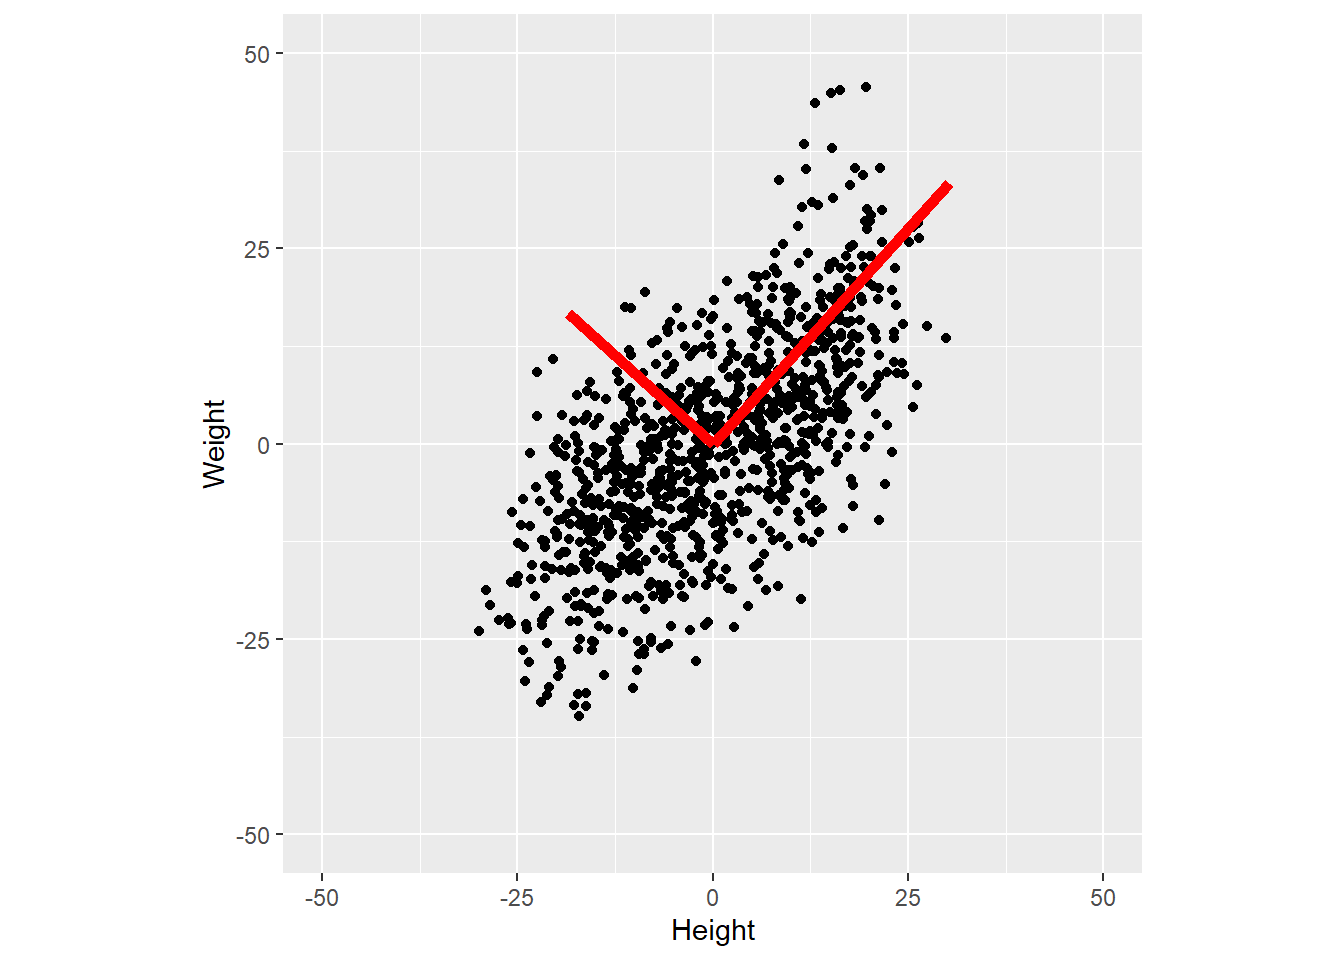
\includegraphics{cohen-linear-algebra_files/figure-latex/e19-1-1.pdf}

\hypertarget{exercise-2-13}{%
\subsection*{Exercise 2}\label{exercise-2-13}}
\addcontentsline{toc}{subsection}{Exercise 2}

\begin{Shaded}
\begin{Highlighting}[]
\NormalTok{X \textless{}{-}}\StringTok{ }\KeywordTok{apply}\NormalTok{(X, }\DataTypeTok{MARGIN=}\DecValTok{2}\NormalTok{, scale, }\DataTypeTok{scale=}\OtherTok{FALSE}\NormalTok{)}
\NormalTok{svdX \textless{}{-}}\StringTok{ }\KeywordTok{svd}\NormalTok{(X, }\DataTypeTok{nu=}\KeywordTok{nrow}\NormalTok{(X), }\DataTypeTok{nv=}\KeywordTok{ncol}\NormalTok{(X))}
\NormalTok{scores \textless{}{-}}\StringTok{ }\NormalTok{X }\OperatorTok{\%*\%}\StringTok{ }\NormalTok{svdX}\OperatorTok{$}\NormalTok{v}
\NormalTok{s \textless{}{-}}\StringTok{ }\KeywordTok{diag}\NormalTok{(svdX}\OperatorTok{$}\NormalTok{d)}\OperatorTok{\^{}}\DecValTok{2} \OperatorTok{/}\StringTok{ }\NormalTok{(}\KeywordTok{nrow}\NormalTok{(X) }\OperatorTok{{-}}\StringTok{ }\DecValTok{1}\NormalTok{)}
\NormalTok{s \textless{}{-}}\StringTok{ }\DecValTok{100} \OperatorTok{*}\StringTok{ }\NormalTok{s }\OperatorTok{/}\StringTok{ }\KeywordTok{sum}\NormalTok{(s) }\CommentTok{\# s == eigvals}
\end{Highlighting}
\end{Shaded}

\hypertarget{exercise-3-6}{%
\subsection*{Exercise 3}\label{exercise-3-6}}
\addcontentsline{toc}{subsection}{Exercise 3}

\begin{Shaded}
\begin{Highlighting}[]
\KeywordTok{library}\NormalTok{(ggplot2)}

\CommentTok{\# create data}
\NormalTok{N \textless{}{-}}\StringTok{ }\DecValTok{1000}
\NormalTok{h \textless{}{-}}\StringTok{ }\KeywordTok{rnorm}\NormalTok{(}\DataTypeTok{n=}\NormalTok{N, }\DataTypeTok{mean =} \KeywordTok{seq}\NormalTok{(}\DecValTok{150}\NormalTok{, }\DecValTok{190}\NormalTok{, }\DataTypeTok{length.out =}\NormalTok{ N), }\DataTypeTok{sd=}\DecValTok{5}\NormalTok{)}
\NormalTok{w \textless{}{-}}\StringTok{ }\NormalTok{h }\OperatorTok{*}\StringTok{ }\FloatTok{.7} \OperatorTok{{-}}\StringTok{ }\DecValTok{50} \OperatorTok{+}\StringTok{ }\KeywordTok{rnorm}\NormalTok{(N, }\DataTypeTok{mean=}\DecValTok{0}\NormalTok{, }\DataTypeTok{sd=}\DecValTok{10}\NormalTok{)}

\CommentTok{\# covariance}
\NormalTok{X \textless{}{-}}\StringTok{ }\KeywordTok{cbind}\NormalTok{(h, w)}
\NormalTok{C \textless{}{-}}\StringTok{ }\KeywordTok{t}\NormalTok{(X) }\OperatorTok{\%*\%}\StringTok{ }\NormalTok{X }\OperatorTok{/}\StringTok{ }\NormalTok{(}\KeywordTok{length}\NormalTok{(h) }\OperatorTok{{-}}\StringTok{ }\DecValTok{1}\NormalTok{)}

\CommentTok{\# PCA}
\NormalTok{eigC \textless{}{-}}\StringTok{ }\KeywordTok{eigen}\NormalTok{(C)}

\CommentTok{\# sorting below is redundant in R, as values and vectors are presorted}
\NormalTok{i \textless{}{-}}\StringTok{ }\KeywordTok{order}\NormalTok{(eigC}\OperatorTok{$}\NormalTok{values, }\DataTypeTok{decreasing=}\OtherTok{TRUE}\NormalTok{) }
\NormalTok{V \textless{}{-}}\StringTok{ }\NormalTok{eigC}\OperatorTok{$}\NormalTok{vectors[, i]}
\NormalTok{eigvals \textless{}{-}}\StringTok{ }\NormalTok{eigC}\OperatorTok{$}\NormalTok{values[i]}
\NormalTok{eigvals \textless{}{-}}\StringTok{ }\DecValTok{100} \OperatorTok{*}\StringTok{ }\NormalTok{eigvals }\OperatorTok{/}\StringTok{ }\KeywordTok{sum}\NormalTok{(eigvals)}
\NormalTok{scores \textless{}{-}}\StringTok{ }\NormalTok{X }\OperatorTok{\%*\%}\StringTok{ }\NormalTok{V }\CommentTok{\# not used, but useful code}

\CommentTok{\# now we center the data}
\NormalTok{X \textless{}{-}}\StringTok{ }\KeywordTok{apply}\NormalTok{(X, }\DataTypeTok{MARGIN=}\DecValTok{2}\NormalTok{, scale, }\DataTypeTok{scale=}\OtherTok{FALSE}\NormalTok{)}

\CommentTok{\# plot data with PCs}
\KeywordTok{ggplot}\NormalTok{(}\DataTypeTok{data=}\OtherTok{NULL}\NormalTok{, }\KeywordTok{aes}\NormalTok{(}\DataTypeTok{x =}\NormalTok{ X[, }\DecValTok{1}\NormalTok{], }\DataTypeTok{y =}\NormalTok{ X[, }\DecValTok{2}\NormalTok{])) }\OperatorTok{+}\StringTok{ }
\StringTok{  }\KeywordTok{geom\_point}\NormalTok{() }\OperatorTok{+}\StringTok{ }
\StringTok{  }\KeywordTok{geom\_segment}\NormalTok{(}\KeywordTok{aes}\NormalTok{(}\DataTypeTok{x=}\DecValTok{0}\NormalTok{, }\DataTypeTok{y=}\DecValTok{0}\NormalTok{, }\DataTypeTok{xend=}\NormalTok{V[}\DecValTok{1}\NormalTok{, }\DecValTok{1}\NormalTok{] }\OperatorTok{*}\StringTok{ }\DecValTok{45}\NormalTok{, }\DataTypeTok{yend=}\NormalTok{V[}\DecValTok{2}\NormalTok{, }\DecValTok{1}\NormalTok{] }\OperatorTok{*}\StringTok{ }\DecValTok{45}\NormalTok{), }\DataTypeTok{color=}\StringTok{"red"}\NormalTok{, }\DataTypeTok{size=}\DecValTok{2}\NormalTok{) }\OperatorTok{+}
\StringTok{  }\KeywordTok{geom\_segment}\NormalTok{(}\KeywordTok{aes}\NormalTok{(}\DataTypeTok{x=}\DecValTok{0}\NormalTok{, }\DataTypeTok{y=}\DecValTok{0}\NormalTok{, }\DataTypeTok{xend=}\NormalTok{V[}\DecValTok{1}\NormalTok{, }\DecValTok{2}\NormalTok{] }\OperatorTok{*}\StringTok{ }\DecValTok{25}\NormalTok{, }\DataTypeTok{yend=}\NormalTok{V[}\DecValTok{2}\NormalTok{, }\DecValTok{2}\NormalTok{] }\OperatorTok{*}\StringTok{ }\DecValTok{25}\NormalTok{), }\DataTypeTok{color=}\StringTok{"red"}\NormalTok{, }\DataTypeTok{size=}\DecValTok{2}\NormalTok{) }\OperatorTok{+}
\StringTok{  }\KeywordTok{scale\_x\_continuous}\NormalTok{(}\DataTypeTok{name=}\StringTok{"Height"}\NormalTok{, }\DataTypeTok{limits=}\KeywordTok{c}\NormalTok{(}\OperatorTok{{-}}\DecValTok{50}\NormalTok{, }\DecValTok{50}\NormalTok{)) }\OperatorTok{+}\StringTok{ }
\StringTok{  }\KeywordTok{scale\_y\_continuous}\NormalTok{(}\DataTypeTok{name=}\StringTok{"Weight"}\NormalTok{, }\DataTypeTok{limits=}\KeywordTok{c}\NormalTok{(}\OperatorTok{{-}}\DecValTok{50}\NormalTok{, }\DecValTok{50}\NormalTok{)) }\OperatorTok{+}\StringTok{ }
\StringTok{  }\KeywordTok{coord\_equal}\NormalTok{()}
\end{Highlighting}
\end{Shaded}

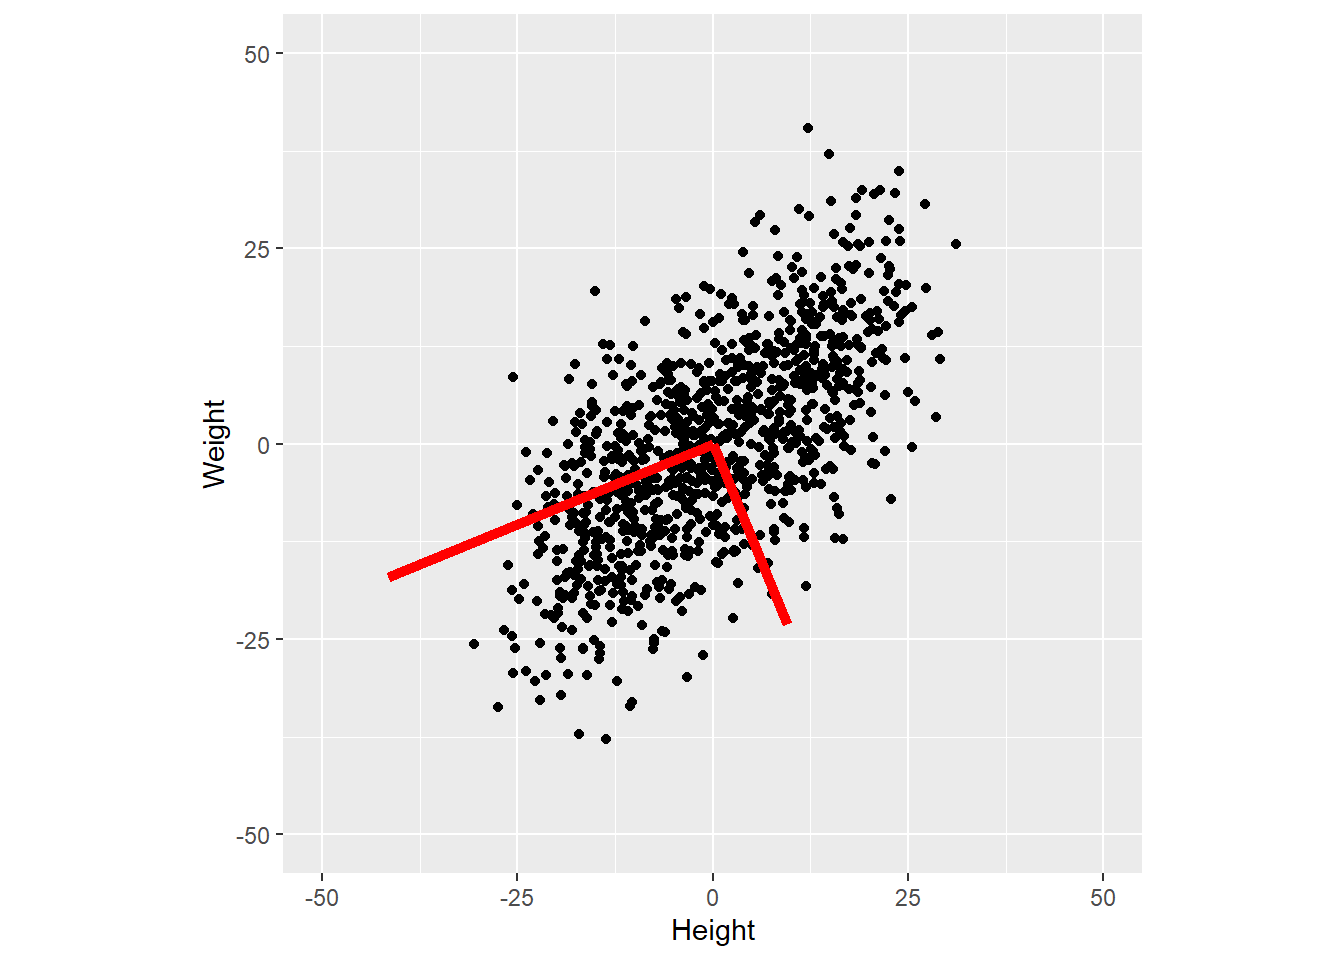
\includegraphics{cohen-linear-algebra_files/figure-latex/e19-3-1.pdf}

\hypertarget{function-references}{%
\chapter*{Function references}\label{function-references}}
\addcontentsline{toc}{chapter}{Function references}

\hypertarget{c}{%
\section*{C}\label{c}}
\addcontentsline{toc}{section}{C}

\begin{itemize}
\tightlist
\item
  Complex numbers in R: \href{https://stat.ethz.ch/R-manual/R-patched/library/base/html/complex.html}{complex()}
\item
  Complex conjugate: \href{https://stat.ethz.ch/R-manual/R-patched/library/base/html/complex.html}{Conj()}
\item
  Concatenating matrices by columns \href{https://stat.ethz.ch/R-manual/R-patched/library/base/html/cbind.html}{cbind()} or rows \href{https://stat.ethz.ch/R-manual/R-patched/library/base/html/cbind.html}{rbind()}
\item
  Condition of matrix: \href{https://rdrr.io/rforge/pracma/man/cond.html}{pracma::cond()}
\item
  Cross product: \href{https://stat.ethz.ch/R-manual/R-patched/library/base/html/crossprod.html}{crossprod()}
\end{itemize}

\hypertarget{d}{%
\section*{D}\label{d}}
\addcontentsline{toc}{section}{D}

\begin{itemize}
\tightlist
\item
  Determinant: \href{https://stat.ethz.ch/R-manual/R-patched/library/base/html/det.html}{det()}
\item
  Diagonal: \href{https://stat.ethz.ch/R-manual/R-patched/library/base/html/diag.html}{diag()}
\item
  Dot product: \href{https://rdrr.io/rforge/pracma/man/dot.html}{pracma::dot()}
\end{itemize}

\hypertarget{e}{%
\section*{E}\label{e}}
\addcontentsline{toc}{section}{E}

\begin{itemize}
\tightlist
\item
  Eigenvalues and eigenvectors: \href{https://stat.ethz.ch/R-manual/R-devel/library/base/html/eigen.html}{eigen()}
\end{itemize}

\hypertarget{g}{%
\section*{G}\label{g}}
\addcontentsline{toc}{section}{G}

\begin{itemize}
\tightlist
\item
  Generalized Eigenvalues: \href{https://rdrr.io/cran/geigen/man/geigen.html}{giegen::geigen()}
\end{itemize}

\hypertarget{h}{%
\section*{H}\label{h}}
\addcontentsline{toc}{section}{H}

\begin{itemize}
\tightlist
\item
  Hankel matrix: \href{https://rdrr.io/rforge/pracma/man/hankel.html}{pracma::hankel()}
\end{itemize}

\hypertarget{i}{%
\section*{I}\label{i}}
\addcontentsline{toc}{section}{I}

\begin{itemize}
\tightlist
\item
  Inverse of a matrix: \href{https://stat.ethz.ch/R-manual/R-devel/library/base/html/solve.html}{solve()}
\end{itemize}

\hypertarget{l}{%
\section*{L}\label{l}}
\addcontentsline{toc}{section}{L}

\begin{itemize}
\tightlist
\item
  Least-squares solution to a linear matrix equation: \href{https://stat.ethz.ch/R-manual/R-patched/library/stats/html/lsfit.html}{lsfit()}
\item
  Lower triangular part of a matrix: \href{https://rdrr.io/rforge/pracma/man/tri.html}{pracma::tril()} and \href{https://stat.ethz.ch/R-manual/R-patched/library/base/html/lower.tri.html}{lower.tri()} for logical indexes (excluding diagonal by default).
\item
  LU decomposition: \href{https://rdrr.io/cran/pracma/man/lu.html}{pracma::lu()}
\end{itemize}

\hypertarget{m}{%
\section*{M}\label{m}}
\addcontentsline{toc}{section}{M}

\begin{itemize}
\tightlist
\item
  Matrix, concatenating by columns \href{https://stat.ethz.ch/R-manual/R-patched/library/base/html/cbind.html}{cbind()} or rows \href{https://stat.ethz.ch/R-manual/R-patched/library/base/html/cbind.html}{rbind()}
\item
  Matrix condition: \href{https://rdrr.io/rforge/pracma/man/cond.html}{pracma::cond()}
\item
  Matrix, creating: \href{https://stat.ethz.ch/R-manual/R-patched/library/base/html/matrix.html}{matrix()}
\item
  Matrix, determinant: \href{https://stat.ethz.ch/R-manual/R-patched/library/base/html/det.html}{det()}
\item
  Matrix diagonal: \href{https://stat.ethz.ch/R-manual/R-patched/library/base/html/diag.html}{diag()}
\item
  Matrix dimensions: \href{https://stat.ethz.ch/R-manual/R-patched/library/base/html/dim.html}{dim()}
\item
  Matrix eigenvalues and eigenvectors: \href{https://stat.ethz.ch/R-manual/R-devel/library/base/html/eigen.html}{eigen}
\item
  Matrix inverse: \href{https://stat.ethz.ch/R-manual/R-devel/library/base/html/solve.html}{solve()}
\item
  Matrix is symmetric (real valued) or Hermitian (complex values): \href{https://stat.ethz.ch/R-manual/R-patched/library/base/html/isSymmetric.html}{isSymmetric()}
\item
  Matrix multiplication: \href{https://stat.ethz.ch/R-manual/R-patched/library/base/html/matmult.html}{\%*\%}
\item
  Matrix norm: \href{https://stat.ethz.ch/R-manual/R-patched/library/base/html/norm.html}{norm()}
\item
  Matrix to the power: \href{https://www.rdocumentation.org/packages/matrixcalc/versions/1.0-3/topics/matrix.power}{matrixcalc::matrix.power()}
\item
  Matrix pseudoinverse: \href{https://rdrr.io/cran/pracma/man/pinv.html}{pracma::pinv()}
\item
  Matrix rank: \href{https://rdrr.io/rforge/pracma/man/rank.html}{pracma::Rank()}
\item
  Matrix trace: \href{https://rdrr.io/rforge/pracma/man/trace.html}{pracma::Trace()}
\item
  Matrix, triangular parts. Lower \href{https://rdrr.io/rforge/pracma/man/tri.html}{pracma::tril()} and upper \href{https://rdrr.io/rforge/pracma/man/tri.html}{pracma::triu()}. Logical indexes (excluding diagonal by default): \href{https://stat.ethz.ch/R-manual/R-patched/library/base/html/lower.tri.html}{lower.tri()} and \href{https://stat.ethz.ch/R-manual/R-patched/library/base/html/lower.tri.html}{upper.tri()}.
\end{itemize}

\hypertarget{n}{%
\section*{N}\label{n}}
\addcontentsline{toc}{section}{N}

\begin{itemize}
\tightlist
\item
  Norm of matrix: \href{https://stat.ethz.ch/R-manual/R-patched/library/base/html/norm.html}{norm()}
\item
  Null space: \href{https://rdrr.io/rforge/pracma/man/nullspace.html}{pracma::nullspace()}
\end{itemize}

\hypertarget{o}{%
\section*{O}\label{o}}
\addcontentsline{toc}{section}{O}

\begin{itemize}
\tightlist
\item
  Outer product: \href{https://stat.ethz.ch/R-manual/R-patched/library/base/html/outer.html}{outer()}
\end{itemize}

\hypertarget{p}{%
\section*{P}\label{p}}
\addcontentsline{toc}{section}{P}

\begin{itemize}
\tightlist
\item
  Power function for matrix: \href{https://www.rdocumentation.org/packages/matrixcalc/versions/1.0-3/topics/matrix.power}{matrixcalc::matrix.power()}
\item
  Pseudoinverse: \href{https://rdrr.io/cran/pracma/man/pinv.html}{pracma::pinv()}
\end{itemize}

\hypertarget{q}{%
\section*{Q}\label{q}}
\addcontentsline{toc}{section}{Q}

\begin{itemize}
\tightlist
\item
  QR decomposition: \href{https://stat.ethz.ch/R-manual/R-devel/library/base/html/qr.html}{qr()}. To reconstruct Q, R, or X matrices see \href{https://stat.ethz.ch/R-manual/R-devel/library/base/html/qraux.html}{qr auxiliaries}.
\end{itemize}

\hypertarget{r}{%
\section*{R}\label{r}}
\addcontentsline{toc}{section}{R}

\begin{itemize}
\tightlist
\item
  Random numbers from a normal distribution: \href{https://stat.ethz.ch/R-manual/R-patched/library/stats/html/Normal.html}{rnorm()}
\item
  Random numbers from a uniform distribution: \href{https://stat.ethz.ch/R-manual/R-patched/library/stats/html/Uniform.html}{runif()}
\item
  Rank: \href{https://rdrr.io/rforge/pracma/man/rank.html}{pracma::Rank()}
\item
  Reduced Row Echelon Form: \href{https://rdrr.io/rforge/pracma/src/R/rref.R}{pracma::rref()}
\end{itemize}

\hypertarget{s}{%
\section*{S}\label{s}}
\addcontentsline{toc}{section}{S}

\begin{itemize}
\tightlist
\item
  Sampling from list of numbers (used in the code to sample integers from a range): \href{https://stat.ethz.ch/R-manual/R-patched/library/base/html/sample.html}{sample()}
\item
  Singular value decomposition: \href{https://stat.ethz.ch/R-manual/R-patched/library/base/html/svd.html}{svd()}
\end{itemize}

\hypertarget{t}{%
\section*{T}\label{t}}
\addcontentsline{toc}{section}{T}

\begin{itemize}
\tightlist
\item
  Toeplitz matrix: \href{https://stat.ethz.ch/R-manual/R-patched/library/stats/html/toeplitz.html}{toeplitz()}
\item
  Trace: \href{https://rdrr.io/rforge/pracma/man/trace.html}{pracma::Trace()}
\item
  Transpose: \href{https://stat.ethz.ch/R-manual/R-devel/library/base/html/t.html}{t()}
\item
  Triangular parts of matrix. Lower \href{https://rdrr.io/rforge/pracma/man/tri.html}{pracma::tril()} and upper \href{https://rdrr.io/rforge/pracma/man/tri.html}{pracma::triu()}. Logical indexes (excluding diagonal by default): \href{https://stat.ethz.ch/R-manual/R-patched/library/base/html/lower.tri.html}{lower.tri()} and \href{https://stat.ethz.ch/R-manual/R-patched/library/base/html/lower.tri.html}{upper.tri()}.
\end{itemize}

\hypertarget{u}{%
\section*{U}\label{u}}
\addcontentsline{toc}{section}{U}

\begin{itemize}
\tightlist
\item
  Upper triangular part of a matrix: \href{https://rdrr.io/rforge/pracma/man/tri.html}{pracma::triu()} and \href{https://stat.ethz.ch/R-manual/R-patched/library/base/html/lower.tri.html}{upper.tri()} for logical indexes (excluding diagonal by default).
\end{itemize}

\hypertarget{v}{%
\section*{V}\label{v}}
\addcontentsline{toc}{section}{V}

\begin{itemize}
\tightlist
\item
  Vector, creating or converting to an atomic vector: \href{https://stat.ethz.ch/R-manual/R-patched/library/base/html/c.html}{c()}
\item
  Vector, converting to an atomic vector: \href{https://stat.ethz.ch/R-manual/R-patched/library/base/html/vector.html}{as.vector()}
\end{itemize}

  \bibliography{book.bib,packages.bib}

\end{document}
